\documentclass[11pt,a4paper,twoside]{book}\usepackage[]{graphicx}\usepackage[]{color}
%% maxwidth is the original width if it is less than linewidth
%% otherwise use linewidth (to make sure the graphics do not exceed the margin)
\makeatletter
\def\maxwidth{ %
  \ifdim\Gin@nat@width>\linewidth
    \linewidth
  \else
    \Gin@nat@width
  \fi
}
\makeatother

\definecolor{fgcolor}{rgb}{0.345, 0.345, 0.345}
\newcommand{\hlnum}[1]{\textcolor[rgb]{0.686,0.059,0.569}{#1}}%
\newcommand{\hlstr}[1]{\textcolor[rgb]{0.192,0.494,0.8}{#1}}%
\newcommand{\hlcom}[1]{\textcolor[rgb]{0.678,0.584,0.686}{\textit{#1}}}%
\newcommand{\hlopt}[1]{\textcolor[rgb]{0,0,0}{#1}}%
\newcommand{\hlstd}[1]{\textcolor[rgb]{0.345,0.345,0.345}{#1}}%
\newcommand{\hlkwa}[1]{\textcolor[rgb]{0.161,0.373,0.58}{\textbf{#1}}}%
\newcommand{\hlkwb}[1]{\textcolor[rgb]{0.69,0.353,0.396}{#1}}%
\newcommand{\hlkwc}[1]{\textcolor[rgb]{0.333,0.667,0.333}{#1}}%
\newcommand{\hlkwd}[1]{\textcolor[rgb]{0.737,0.353,0.396}{\textbf{#1}}}%
\let\hlipl\hlkwb

\usepackage{framed}
\makeatletter
\newenvironment{kframe}{%
 \def\at@end@of@kframe{}%
 \ifinner\ifhmode%
  \def\at@end@of@kframe{\end{minipage}}%
  \begin{minipage}{\columnwidth}%
 \fi\fi%
 \def\FrameCommand##1{\hskip\@totalleftmargin \hskip-\fboxsep
 \colorbox{shadecolor}{##1}\hskip-\fboxsep
     % There is no \\@totalrightmargin, so:
     \hskip-\linewidth \hskip-\@totalleftmargin \hskip\columnwidth}%
 \MakeFramed {\advance\hsize-\width
   \@totalleftmargin\z@ \linewidth\hsize
   \@setminipage}}%
 {\par\unskip\endMakeFramed%
 \at@end@of@kframe}
\makeatother

\definecolor{shadecolor}{rgb}{.97, .97, .97}
\definecolor{messagecolor}{rgb}{0, 0, 0}
\definecolor{warningcolor}{rgb}{1, 0, 1}
\definecolor{errorcolor}{rgb}{1, 0, 0}
\newenvironment{knitrout}{}{} % an empty environment to be redefined in TeX

\usepackage{alltt}
% We load package by package and set package relevant parameters.
% Topics are summarized later
%%%%%%%%%%%%%%%%%%%%%%%%%%%%%%%%%%%%%%%%%%%%%%%%%%%%%%%%%%%%%%%%%%%%%%%%
% helping packages
\usepackage{ifthen}
\usepackage{calc}

\usepackage[T1]{fontenc}       % provides fonts having  accented characters 
\usepackage[latin1]{inputenc}  % allows the user to input accented characters directly from the keyboard

%%%%%%%%%%%%%%%%%%%%%%%%%%%%%%%%%%%%%%%%%%%%%%%%%%%%%%%%%%%%%%%%%%%%%%%%

\renewcommand{\baselinestretch}{1.2}
\renewcommand{\textfraction}{0}%0.2     % placement of figures
\renewcommand{\topfraction}{1}%.3
\renewcommand{\bottomfraction}{1}%.3
\renewcommand{\floatpagefraction}{1}%.3
\setcounter{bottomnumber}{3}%1

\textwidth6.3in
\textheight9.7in
\topmargin-45pt
\oddsidemargin-.15in
\evensidemargin.15in
\headsep30pt
\headheight15pt
%\footskip20pt


%%%%%%%%%%%%%%%%%%%%%%%%%%%%%%%%%%%%%%%%%%%%%%%%%%%%%%%%%%%%%%%%%%%%%%%%

\usepackage[dvipsnames]{xcolor}
\definecolor{fgcolor}{rgb}{0.345, 0.345, 0.345}
\definecolor{shadecolor}{rgb}{.97, .97, .97}
\definecolor{messagecolor}{rgb}{0, 0, 0}
\definecolor{warningcolor}{rgb}{1, 0, 1}
\definecolor{errorcolor}{rgb}{1, 0, 0}
\definecolor{DarkBlue}{rgb}{0,0,0.5451}
\definecolor{DarkGreen}{rgb}{0,0.39216,0}
\definecolor{LightYellow}{rgb}{1,1,.8}
\definecolor{orange}{rgb}{.9,0.3445,0}



%%%%%%%%%%%%%%%%%%%%%%%%%%%%%%%%%%%%%%%%%%%%%%%%%%%%%%%%%%%%%%%%%%%%%%%%
\usepackage{afterpage}
\usepackage{natbib}
\usepackage{upquote}

\usepackage[english]{babel}

%%%%%%%%%%%%%%%%%%%%%%%%%%%%%%%%%%%%%%%%%%%%%%%%%%%%%%%%%%%%%%%%%%%%%%%%%%%%%%%
%% maxwidth is the original width if it is less than linewidth
%% otherwise use linewidth (to make sure the graphics do not exceed the margin)
\makeatletter
\def\maxwidth{ %
  \ifdim\Gin@nat@width>\linewidth
    \linewidth
  \else
    \Gin@nat@width
  \fi
}
\makeatother

%%%%%%%%%%%%%%%%%%%%%%%%%%%%%%%%%%%%%%%%%%%%%%%%%%%%%%%%%%%%%%%%%%%%%%%%%%%%%%%%%%%%%%%%%%%%%%%%%%%%%%%%%%%%
% from fancyvrb
\usepackage{fancyhdr}
\usepackage{fancyvrb}
\DefineVerbatimEnvironment{Rcode}{Verbatim}{xleftmargin=2em,fontshape=sl,formatcom=\color{DarkGreen}}
\fvset{listparameters={\setlength{\topsep}{0pt}}}

%%%%%%%%%%%%%%%%%%%%%%%%%%%%%%%%%%%%%%%%%%%%%%%%%%%%%%%%%%%%%%%%%%%%%%%%%%%%%%%%%%%%%%%%%%%%%%%%%%%%%%%%%%%%%
\usepackage{float}
\usepackage{graphicx}
\usepackage[margin=2em,labelfont=bf]{caption}


%%%%%%%%%%%%%%%%%%%%%%%%%%%%%%%%%%%%%%%%%%%%%%%%%%%%%%%%%%%%%%%%%%%%%%%%
\usepackage[pdftex,plainpages=false,pdfpagelabels,pagebackref=true,colorlinks=true,pdfpagemode=UseOutlines]{hyperref}


%%%%%%%%
\usepackage{tabularx}
%%%%%%%%

%%%%%%%%%%%%%%%%%%%%%%%%%%%%%%%%%%%%%%%%%%%%%%%%%%%%%%%%%%%%%%%%%%%%%%%%
% now math stuff and other details...
\usepackage{amsmath,amsthm,amssymb}

\newtheorem{pro}{Property}[chapter]
\theoremstyle{definition}
\newtheorem{des}{Definition}[chapter]
\newtheorem{bsp}{Example}[chapter]
\newtheorem{rem}{Remark}[chapter]

\newcommand*\widebar[1]{%
  \vbox{%
    \hrule height 0.5pt%     % Line above with certain width
    \kern0.5ex%             % Distance between line and content
    \hbox{%
      \kern-0.1em%           % Distance between content and left side of box, negative values for lines shorter than content
      \ifmmode#1\else\ensuremath{#1}\fi%  % The content, typeset in dependence of mode
      \kern-0.1em%      % Distance between content and left side of box, negative values for lines shorter than content
    }% end of hbox
  }% end of vbox
}
\def\ds{\displaystyle}

\newcommand{\rr}[1]{{\ttfamily\slshape\color{DarkGreen} #1}}

\makeatletter


% clever trick to circumvent potential redefines after loading packages:
% \providecommand{\something}{}  % if it does not exist, it creates it.
%      has same syntax as \newcommand
% \renewcommand{\something}{....}
% TUGboat 29(2)


\makeatletter
%umdefinierung exisitierender befehle
\let\oldH\H
\let\oldL\L
\let\oldO\H
\let\oldS\S
\let\olda\a
\let\oldb\b
\let\oldc\c
\let\oldd\d
\let\oldk\k
\let\oldv\v
\let\oldl\l
\let\oldt\t
\let\oldu\u
\let\oldIJ\IJ
\let\oldP\P
\let\P\relax
\let\oldnorm\|

%\DefineVerbatimEnvironment{CodeInput}{Verbatim}{fontshape=sl}
%\DefineVerbatimEnvironment{CodeOutput}{Verbatim}{}

% some classical environments, up-right, with chapter numbering.
\theoremstyle{definition}
\newtheorem{definition}{Definition}[chapter]
\newtheorem{example}{Example}[chapter]
\newtheorem{remark}{Remark}[chapter]
\newtheorem{theorem}{Theorem}[chapter]



\renewcommand{\|}{|\!|}         % closer norm
\newcommand{\T}{{}^{\top}}
\newcommand\code[1]{{\tt#1}}



\newcounter{algo}
\newenvironment{algorithm}{%
  \begin{list}{
      (\arabic{algo})
    }{
      \usecounter{algo}
    }%
}{
  \end{list}
}

% some text abbreviation
\newcommand{\GLS}{\text{GLS}}
\newcommand{\RR}{\text{RR}}
\newcommand{\OR}{\text{OR}}
\newcommand{\WLS}{\text{WLS}}
\newcommand{\MLE}{\text{MLE}}
\newcommand{\OLS}{\text{OLS}}
\newcommand{\MAE}{\text{MAE}}
\newcommand{\MAD}{\text{MAD}}
\newcommand{\RMSE}{\text{RMSE}}
\newcommand{\SVAR}{\text{svar}} %silvanos new commands
\newcommand{\EVAR}{\text{evar}}
\newcommand{\LMG}{\text{LMG}}
\newcommand{\Rtwo}{\text{R}^2}



\newcommand{\ii}{\text{\i}}

\newcommand{\Bin}{\cB\mathit{\!i\!n}}
\newcommand{\Beta}{\cB\mathit{\!e\!t\!a}}
\newcommand{\Pois}{\cP\mathit{\!o\!i\!s\!s\!o\!n}}
\newcommand{\Exp}{\cE\mathit{\!x\!p}}


\DeclareMathOperator*{\argmin}{argmin}
\DeclareMathOperator*{\argmax}{argmax}
\DeclareMathOperator{\diag}{diag}
\DeclareMathOperator{\diam}{diam}
\DeclareMathOperator{\card}{card}
\DeclareMathOperator{\cov}{Cov}                   
\DeclareMathOperator{\corr}{Corr}                 
\DeclareMathOperator{\var}{Var}                   
\DeclareMathOperator{\trace}{tr}                  
\DeclareMathOperator{\E}{E}                       
\DeclareMathOperator{\P}{P}                       
\DeclareMathOperator{\pred}{p}
\DeclareMathOperator{\vect}{vec}                  
\DeclareMathOperator{\vech}{vech}                 
\DeclareMathOperator{\rank}{rank}                 
\DeclareMathOperator{\e}{e}                       
%\DeclareMathOperator{\cv}{CV}                     
\DeclareMathOperator{\GCV}{GCV}                     
\DeclareMathOperator{\CV}{CV}                     
\DeclareMathOperator{\BLUP}{BLUP}                 
\DeclareMathOperator{\MSE}{MSE}                   
\DeclareMathOperator{\MS}{MS}                   
\DeclareMathOperator{\df}{df}                   
\DeclareMathOperator{\bias}{bias}                   
\DeclareMathOperator{\eig}{eig}                   
\DeclareMathOperator{\Prec}{Prec}
\DeclareMathOperator{\mode}{mode}
\renewcommand{\SS}{\text{SS}}
\renewcommand{\d}{\mathsf{\,d}}

\def\arctanh{\qopname\relax o{arctanh}}  % as in amsopn
\newcommand{\bigo}{\cO}
\newcommand{\lito}{\text{\scriptsize{$\cO$}}}
\newcommand{\cdfPhi}{\itPhi}
\newcommand{\ml}{_\text{ML}}

\newcommand*{\stack@relbin}[3][]{%
  \mathop{#3}\limits
  \toks@{#1}%
  \edef\reserved@a{\the\toks@}%
  \ifx\reserved@a\@empty\else_{#1}\fi
  \toks@{#2}%
  \edef\reserved@a{\the\toks@}%
  \ifx\reserved@a\@empty\else^{#2}\fi
  \egroup
}%
\renewcommand*{\stackrel}{\mathrel\bgroup\stack@relbin}
\newcommand*{\stackbin}{\mathbin\bgroup\stack@relbin}
\newcommand{\simiid}{\stackrel[]{\text{iid}}{\sim}}

% Kalligraphischer Schriftsatz
\newcommand{\cA}{{\cal{A}}}
\newcommand{\cB}{{\cal{B}}} 
\newcommand{\cC}{{\cal{C}}}
\newcommand{\cD}{{\cal{D}}} 
\newcommand{\cE}{{\cal{E}}}
\newcommand{\cF}{{\cal{F}}}
\newcommand{\cG}{{\cal{G}}}
\newcommand{\cH}{{\cal{H}}}
\newcommand{\cI}{{\cal{I}}}
\newcommand{\cJ}{{\cal{J}}}
\newcommand{\cK}{{\cal{K}}}
\newcommand{\cL}{{\cal{L}}}
\newcommand{\cM}{{\cal{M}}} 
\newcommand{\cN}{{\cal{N}}}
\newcommand{\cO}{{\cal{O}}} 
\newcommand{\cP}{{\cal{P}}}
\newcommand{\cQ}{{\cal{Q}}} 
\newcommand{\cR}{{\cal{R}}} 
\newcommand{\cS}{{\cal{S}}} 
\newcommand{\cT}{{\cal{T}}}
\newcommand{\cU}{{\cal{U}}}
\newcommand{\cV}{{\cal{V}}}
\newcommand{\cW}{{\cal{W}}}
\newcommand{\cX}{{\cal{X}}} 
\newcommand{\cY}{{\cal{Y}}}
\newcommand{\cZ}{{\cal{Z}}} 


\newcommand{\IA}{{\mathbb{A}}}
\newcommand{\IB}{{\mathbb{B}}}
\newcommand{\IC}{{\mathbb{C}}}
\newcommand{\ID}{{\mathbb{D}}}
\newcommand{\IE}{{\mathbb{E}}}
\newcommand{\IF}{{\mathbb{F}}}
\newcommand{\IG}{{\mathbb{G}}}
\newcommand{\IH}{{\mathbb{H}}}
\newcommand{\II}{{\mathbb{I}}}
%\newcommand{\IJ}{{\mathbb{J}}}
\newcommand{\IK}{{\mathbb{K}}}
\newcommand{\IL}{{\mathbb{L}}}
\newcommand{\IM}{{\mathbb{M}}}
\newcommand{\IN}{{\mathbb{N}}}
\newcommand{\IO}{{\mathbb{O}}}
\newcommand{\IP}{{\mathbb{P}}}
\newcommand{\IQ}{{\mathbb{Q}}}
\newcommand{\IR}{{\mathbb{R}}}
\newcommand{\IS}{{\mathbb{S}}}
\newcommand{\IT}{{\mathbb{T}}}
\newcommand{\IU}{{\mathbb{U}}}
\newcommand{\IV}{{\mathbb{V}}}
\newcommand{\IW}{{\mathbb{W}}}
\newcommand{\IX}{{\mathbb{X}}}
\newcommand{\IY}{{\mathbb{Y}}}
\newcommand{\IZ}{{\mathbb{Z}}}


% fette griechische kleinbuchstaben
\newcommand{\balpha}{{\boldsymbol{\alpha}}}
\newcommand{\bbeta}{{\boldsymbol{\beta}}}
\newcommand{\bgamma}{{\boldsymbol{\gamma}}}
\newcommand{\bdelta}{{\boldsymbol{\delta}}}
\newcommand{\blambda}{{\boldsymbol{\lambda}}}
\newcommand{\bepsilon}{{\boldsymbol{\epsilon}}}
\newcommand{\bvarepsilon}{{\boldsymbol{\varepsilon}}}
\newcommand{\bzeta}{{\boldsymbol{\zeta}}}
\newcommand{\bfeta}{{\boldsymbol{\eta}}}  %  <----- exception !
\newcommand{\btheta}{{\boldsymbol{\theta}}{}}
\newcommand{\bvartheta}{{\boldsymbol{\vartheta}}}
\newcommand{\biota}{{\boldsymbol{\iota}}}
\newcommand{\bkappa}{{\boldsymbol{\kappa}}}
\newcommand{\bmu}{{\boldsymbol{\mu}}}
\newcommand{\bnu}{{\boldsymbol{\nu}}}
\newcommand{\bxi}{{\boldsymbol{\xi}}}
\newcommand{\bpi}{{\boldsymbol{\pi}}}
\newcommand{\bvarpi}{{\boldsymbol{\varpi}}}
\newcommand{\brho}{{\boldsymbol{\rho}}}
\newcommand{\bvarrhoi}{{\boldsymbol{\varrho}}}
\newcommand{\bsigma}{{\boldsymbol{\sigma}}}
\newcommand{\bvarsigma}{{\boldsymbol{\varsigma}}}
\newcommand{\btau}{{\boldsymbol{\tau}}}
\newcommand{\bvartau}{{\boldsymbol{\vartau}}}
\newcommand{\bupsilon}{{\boldsymbol{\upsilon}}}
\newcommand{\bphi}{{\boldsymbol{\phi}}}
\newcommand{\bvarphi}{{\boldsymbol{\varphi}}}
\newcommand{\bchi}{{\boldsymbol{\chi}}}
\newcommand{\bpsi}{{\boldsymbol{\psi}}}
\newcommand{\bomega}{{\boldsymbol{\omega}}}


% fette griechische grossbuchstaben
\newcommand{\bGamma}{{\boldsymbol{\Gamma}}}
\newcommand{\bDelta}{{\boldsymbol{\Delta}}}
\newcommand{\bTheta}{{\boldsymbol{\Theta}}}
\newcommand{\bLambda}{{\boldsymbol{\Lambda}}{}}
\newcommand{\bXi}{{\boldsymbol{\Xi}}}
\newcommand{\bPi}{{\boldsymbol{\Pi}}}
\newcommand{\bSigma}{{\boldsymbol{\Sigma}}{}}
\newcommand{\bUpsilon}{{\boldsymbol{\Upsilon}}{}}
\newcommand{\bPhi}{{\boldsymbol{\Phi}}}
\newcommand{\bPsi}{{\boldsymbol{\Psi}}}
\newcommand{\bOmega}{{\boldsymbol{\Omega}}}

% italics griechische grossbuchstaben
\newcommand{\itGamma}{{\mathit{\Gamma}}}
\newcommand{\itDelta}{{\mathit{\Delta}}}
\newcommand{\itTheta}{{\mathit{\Theta}}}
\newcommand{\itLambda}{{\mathit{\Lambda}}}
\newcommand{\itXi}{{\mathit{\Xi}}}
\newcommand{\itPi}{{\mathit{\Pi}}}
\newcommand{\itSigma}{{\mathit{\Sigma}}}
\newcommand{\itUpsilon}{{\mathit{\Upsilon}}}
\newcommand{\itPhi}{{\mathit{\Phi}}}
\newcommand{\itPsi}{{\mathit{\Psi}}}
\newcommand{\itOmega}{{\mathit{\Omega}}}



\newcommand{\A}{{\mathbf{A}}}
\newcommand{\B}{{\mathbf{B}}}
\newcommand{\C}{{\mathbf{C}}}
\newcommand{\D}{{\mathbf{D}}}
\newcommand{\bfE}{{\mathbf{E}}}    % \E: expectation
\newcommand{\F}{{\mathbf{F}}}
\newcommand{\G}{{\mathbf{G}}}
\renewcommand{\H}{{\mathbf{H}}}
\newcommand{\I}{{\mathbf{I}}}
\newcommand{\J}{{\mathbf{J}}}
\newcommand{\K}{{\mathbf{K}}}
\renewcommand{\L}{{\mathbf{L}}}
\newcommand{\bfM}{{\mathbf{M}}}
\newcommand{\N}{{\mathbf{N}}}
\renewcommand{\O}{{\mathbf{O}}}
\newcommand{\bfP}{{\mathbf{P}}}  % \P : probability
\newcommand{\Q}{{\mathbf{Q}}}
\newcommand{\bfR}{{\mathbf{R}}}
\renewcommand{\S}{{\mathbf{S}}}
\newcommand{\bfT}{{\mathbf{T}}} % \T transpose
\newcommand{\U}{{\mathbf{U}}}
\newcommand{\V}{{\mathbf{V}}}
\newcommand{\W}{{\mathbf{W}}}
\newcommand{\X}{{\mathbf{X}}}
\newcommand{\Y}{{\mathbf{Y}}}
\newcommand{\Z}{{\mathbf{Z}}}


\newcommand{\0}{{\mathbf{0}}}
\newcommand{\1}{{\mathbf{1}}}
\newcommand{\2}{{\mathbf{2}}}
\newcommand{\3}{{\mathbf{3}}}
\newcommand{\4}{{\mathbf{4}}}
\newcommand{\5}{{\mathbf{5}}}
\newcommand{\6}{{\mathbf{6}}}
\newcommand{\7}{{\mathbf{7}}}
\newcommand{\8}{{\mathbf{8}}}
\newcommand{\9}{{\mathbf{9}}}

\renewcommand{\a}{{\textbf{\textit{a}}}}
\renewcommand{\b}{{\textbf{\textit{b}}}}
\renewcommand{\c}{{\textbf{\textit{c}}}}
\newcommand{\bfd}{{\textbf{\textit{d}}}}  % \d  'dx'
\newcommand{\bfe}{{\textbf{\textit{e}}}}  % \e  l'exponentiel
\newcommand{\f}{{\textbf{\textit{f}}}}
\newcommand{\g}{{\textbf{\textit{g}}}}
\newcommand{\h}{{\textbf{\textit{h}}}}
\newcommand{\bfi}{{\textbf{\textit{i}}}}%\i  complex i, sans 'dot'
\newcommand{\bfj}{{\textbf{\textit{j}}}}
\renewcommand{\l}{{\textbf{\textit{l}}}}
\renewcommand{\k}{{\textbf{\textit{k}}}}
\newcommand{\m}{{\textbf{\textit{m}}}}
\newcommand{\bfn}{{\textbf{\textit{n}}}}
\newcommand{\bfo}{{\textbf{\textit{o}}}}
\newcommand{\p}{{\textbf{\textit{p}}}}
\newcommand{\q}{{\textbf{\textit{q}}}}
\renewcommand{\r}{{\textbf{\textit{r}}}}
\newcommand{\s}{{\textbf{\textit{s}}}}
\renewcommand{\t}{{\textbf{\textit{t}}}}
\newcommand{\bfu}{{\textbf{\textit{u}}}} %\u used in references
\renewcommand{\v}{{\textbf{\textit{v}}}}
\newcommand{\w}{{\textbf{\textit{w}}}}
\newcommand{\x}{{\textbf{\textit{x}}}}
\newcommand{\y}{{\textbf{\textit{y}}}}
\newcommand{\z}{{\textbf{\textit{z}}}}




\ifcsname hlkwd\endcsname%    ... command '#1' exists ...%
\else%  ... command '#1' does not exist ...%

\def\maxwidth{ %
  \ifdim\Gin@nat@width>\linewidth
    \linewidth
  \else
    \Gin@nat@width
  \fi
}

\definecolor{fgcolor}{rgb}{0.345, 0.345, 0.345}
\newcommand{\hlnum}[1]{\textcolor[rgb]{0.686,0.059,0.569}{#1}}%
\newcommand{\hlstr}[1]{\textcolor[rgb]{0.192,0.494,0.8}{#1}}%
\newcommand{\hlcom}[1]{\textcolor[rgb]{0.678,0.584,0.686}{\textit{#1}}}%
\newcommand{\hlopt}[1]{\textcolor[rgb]{0,0,0}{#1}}%
\newcommand{\hlstd}[1]{\textcolor[rgb]{0.345,0.345,0.345}{#1}}%
\newcommand{\hlkwa}[1]{\textcolor[rgb]{0.161,0.373,0.58}{\textbf{#1}}}%
\newcommand{\hlkwb}[1]{\textcolor[rgb]{0.69,0.353,0.396}{#1}}%
\newcommand{\hlkwc}[1]{\textcolor[rgb]{0.333,0.667,0.333}{#1}}%
\newcommand{\hlkwd}[1]{\textcolor[rgb]{0.737,0.353,0.396}{\textbf{#1}}}%

\usepackage{framed}
\newenvironment{kframe}{%
 \def\at@end@of@kframe{}%
 \ifinner\ifhmode%
  \def\at@end@of@kframe{\end{minipage}}%
  \begin{minipage}{\columnwidth}%
 \fi\fi%
 \def\FrameCommand##1{\hskip\@totalleftmargin \hskip-\fboxsep
 \colorbox{shadecolor}{##1}\hskip-\fboxsep
     % There is no \\@totalrightmargin, so:
     \hskip-\linewidth \hskip-\@totalleftmargin \hskip\columnwidth}%
 \MakeFramed {\advance\hsize-\width
   \@totalleftmargin\z@ \linewidth\hsize
   \@setminipage}}%
 {\par\unskip\endMakeFramed%
 \at@end@of@kframe}
\renewenvironment{kframe}{%
 \def\at@end@of@kframe{}%
 \ifinner\ifhmode%
  \def\at@end@of@kframe{\end{minipage}}%
  \begin{minipage}{\columnwidth}%
 \fi\fi%
 \def\FrameCommand##1{\hskip\@totalleftmargin \hskip-0\fboxsep
 \colorbox{shadecolor}{##1}\hskip-0\fboxsep
     % There is no \\@totalrightmargin, so:
     \hskip-\linewidth \hskip-\@totalleftmargin \hskip\columnwidth}%
 \MakeFramed {\advance\hsize-\width
   \@totalleftmargin\z@ \linewidth\hsize
   \@setminipage}}%
 {\par\unskip\endMakeFramed%
 \at@end@of@kframe}


\definecolor{shadecolor}{rgb}{.97, .97, .97}
\definecolor{messagecolor}{rgb}{0, 0, 0}
\definecolor{warningcolor}{rgb}{1, 0, 1}
\definecolor{errorcolor}{rgb}{1, 0, 0}
%\newenvironment{knitrout}{}{} % an empty environment to be redefined in TeX
\newenvironment{knitrout}{\setlength{\topsep}{0mm}\setlength{\fboxsep}{4mm}}{} 

\usepackage{alltt}
\IfFileExists{upquote.sty}{\usepackage{upquote}}{}

  \fi%

\makeatother
   % packages, layout and standard macros
\IfFileExists{upquote.sty}{\usepackage{upquote}}{}
\begin{document}
\renewcommand\familydefault{\sfdefault} 
\pagenumbering{Alph}


\thispagestyle{empty}
\renewcommand{\baselinestretch}{1.5}\normalfont
\begin{center}
\setlength{\parindent}{0cm}
\bf\Large% 
The variable importance metric LMG  \\
applied to Bayesian linear regression models
\normalfont



\hrulefill

\vspace*{4cm}

\large
Master Thesis in Biostatistics (STA495) % or choose the next one
% Master Thesis in Mathematics (MAT491) 
\vspace*{12mm}

by

\vspace*{12mm}

Silvano Sele\\
\small 09 734 492\\
\normalfont
\vspace*{4cm}

supervised by

\vspace*{1cm}

Dr. Stefanie Muff\\
Name of supervisor (with title and affiliation if external)

\vfill

Zurich, September, 2018
\end{center}
\renewcommand\familydefault{\rmdefault}%
\renewcommand{\baselinestretch}{1.0}\rm 
\setcounter{page}{0}
\newpage
\vspace*{12cm}~\thispagestyle{empty}\pagenumbering{Roman}
\newpage


\graphicspath{{./figure/}}
\DeclareGraphicsExtensions{.pdf,.png}
\setcounter{tocdepth}{1}

\thispagestyle{empty}
\begin{center}
\vspace*{6cm}{\bfseries\Huge
  $p$-values:\\[5mm] their use, abuse and proper use \\[5mm]
  illustrated with seven facets 
}
\vfill
\rm

\LARGE
M\"axli Musterli\\[12mm]

\normalsize
Version \today
\end{center}
\newpage
\thispagestyle{empty}~
\newpage
\pagenumbering{roman}

\thispagestyle{plain}\markboth{Contents}{Contents}
\tableofcontents
\setkeys{Gin}{width=.8\textwidth}

\chapter*{Preface}
\addtocontents{toc}{\protect \vspace*{13.mm}}
\addcontentsline{toc}{chapter}{\bfseries{Preface}}
\thispagestyle{plain}\markboth{Preface}{Preface}

Howdy!

\bigskip

\begin{flushright}
Max Muster\\
June 2018
\end{flushright}

\addtocontents{toc}{\protect \vspace*{10mm}}

\cleardoublepage
\pagenumbering{arabic}


%%%%%%%%%%%%%%%%%%%%%%%%%%%%%%%%%%%%%%%%%%%%%%%%%%%%%%%%%%%%%%%%%%%%%% 



% LaTeX file for Chapter 01







\chapter{Introduction}

The aim of this master thesis is to implement the variable importance measure LMG  (named after the authors Lindeman, Merenda, and Gold \citep{Gromping2007}) in linear models estimated with Bayesian methods. 

Regression models are popular in many applied research areas \citep{Nimon2013}. These models provide a tool to find an association between a response variable Y and a set of explanatory variables. The explanatory variables are also called predictors or covariates. Regression parameters provide us the information how much the response variable is expected to change when a predictor changes by one unit, given all other predictors in the model stay the same. The last subsentence is very important for the correct interpretation of the regression parameters. It shows also that the parameter value of a predictor is dependent on the other predictors in the model.

Because predictors are often correlated to some degree to each other, it is clear that it is not an easy task to find the most important predictors in a model. The first question then is: What do we  mean by the importance of a predictor? A question that is not easy answered and depending on the research question. \cite{Gromping2015} concludes that there may never  be a unique accepted definition of what variable importance is. Different metrics exist to quantify the importance of predictors. These metrics focus on different aspects and with correlated predictors they  lead to different conclusions.  A summary of the metrics can be found in  \cite{Gromping2015}.  

A distinction should be made between the importance of predictors in regression models that are used to predict future data and regression models who wish to find an association between predictors and the response variable. In the former case, the aim is only to reduce the error between the predicted values and the real observed values. It does not really matter how we get there. In the other case, we are interested in the strength of the relationship between the predictors and the response variable. A predictor may explain little of the response variable given two other correlated predictors are already included in a regression model. However, this from the regression output unimportant predictor may be the main cause of the other two predictor values.  It therefore may somehow be the most important predictor in this model \citep{Gromping2007}. 

The causal relationship between the variables is missing in the regression model. Regressing conditional on  other variables or using univariate regression models only provide us some parts of the bigger picture about the predictor in a model. Some authors recommend that the variable importance metric is based on both components.  Which variable importance metrics are the most useful ones is still an open debate. A convincing theoretical basis is still lacking for all of them.  \cite{Gromping2015} recommends to use the existing best practices, until a more profound solution is found. For variance (or genereally goodness of fit) decomposition based importance, she recommends to use LMG enhanced with joint contributions or dominance analysis \citep{Gromping2007}.  


% LaTeX file for Chapter 02








\chapter{Data} 
Maybe it is the methods section. Here however, we give a couple hints.
Note that you can wisely use \rr{preamble}-chunks. Minimal, is likely: 

\bigskip

\hrule
\begin{knitrout}
\definecolor{shadecolor}{rgb}{0.969, 0.969, 0.969}\color{fgcolor}\begin{kframe}
\begin{alltt}
\hlkwd{library}\hlstd{(knitr)}
\hlstd{opts_chunk}\hlopt{$}\hlkwd{set}\hlstd{(}
    \hlkwc{fig.path}\hlstd{=}\hlstr{'figure/ch02_fig'}\hlstd{,}
    \hlkwc{self.contained}\hlstd{=}\hlnum{FALSE}\hlstd{,}
    \hlkwc{cache}\hlstd{=}\hlnum{TRUE}
\hlstd{)}
\end{alltt}
\end{kframe}
\end{knitrout}
\hrule

\bigskip

Defining figure options is very helpful:

 
\bigskip


\hrule
\begin{knitrout}
\definecolor{shadecolor}{rgb}{0.969, 0.969, 0.969}\color{fgcolor}\begin{kframe}
\begin{alltt}
\hlkwd{library}\hlstd{(knitr)}
\hlstd{opts_chunk}\hlopt{$}\hlkwd{set}\hlstd{(}\hlkwc{fig.path}\hlstd{=}\hlstr{'figure/ch02_fig'}\hlstd{,}
               \hlkwc{echo}\hlstd{=}\hlnum{TRUE}\hlstd{,} \hlkwc{message}\hlstd{=}\hlnum{FALSE}\hlstd{,}
               \hlkwc{fig.width}\hlstd{=}\hlnum{8}\hlstd{,} \hlkwc{fig.height}\hlstd{=}\hlnum{2.5}\hlstd{,}
               \hlkwc{out.width}\hlstd{=}\hlstr{'\textbackslash{}\textbackslash{}textwidth-3cm'}\hlstd{,}
               \hlkwc{message}\hlstd{=}\hlnum{FALSE}\hlstd{,} \hlkwc{fig.align}\hlstd{=}\hlstr{'center'}\hlstd{,}
               \hlkwc{background}\hlstd{=}\hlstr{"gray98"}\hlstd{,} \hlkwc{tidy}\hlstd{=}\hlnum{FALSE}\hlstd{,} \hlcom{#tidy.opts=list(width.cutoff=60),}
               \hlkwc{cache}\hlstd{=}\hlnum{TRUE}
\hlstd{)}
\hlkwd{options}\hlstd{(}\hlkwc{width}\hlstd{=}\hlnum{74}\hlstd{)}
\end{alltt}
\end{kframe}
\end{knitrout}
\hrule

\bigskip 

Notice how in Figure~\ref{f02:1} everything is properly scaled.   

\begin{figure}
\begin{knitrout}
\definecolor{shadecolor}{rgb}{0.98, 0.98, 0.98}\color{fgcolor}

{\centering 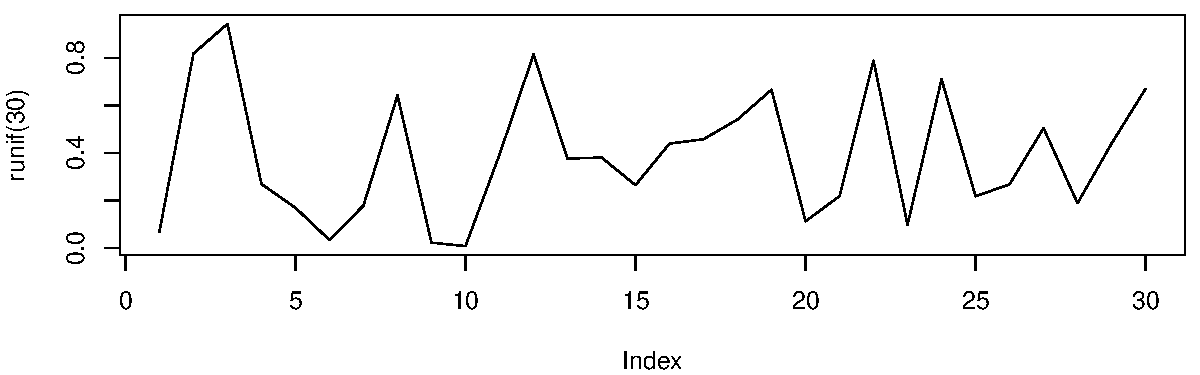
\includegraphics[width=\textwidth-3cm]{figure/ch02_figunnamed-chunk-3-1} 

}



\end{knitrout}
  \caption{Test figure to illustrate figure options used by knitr.}
  \label{f02:1}
\end{figure}


The focus of this master thesis is on the LMG variable importance metric. The LMG is a metric that is based on variance decomposition. The total $\Rtwo$ of a model is decomposed onto the predictors. Many authors call this a desirable property of a variable importance metric. Marginal and conditional information are incorporated \citep{Gromping2015} .  The following formulas are taken from \cite{Gromping2015}. The same mathematical notations are used. 

The following  notations for the explained variance (1) and sequentially added variance (2) simplify the notation of the LMG formula. 

   \begin{align} 
     \EVAR(S) = \var(Y) - \var( Y \mid X_{j}, j \in S),   \label{eq:1} 
   \end{align} 
   \begin{align} 
     \SVAR(M \mid S) = \EVAR(M \cup S) - \EVAR(S), \label{eq:2} 
    \end{align} , where S and M denote disjoint sets of predictors.
    
   The LMG formula is given below for the first predictor only. Because of exchangeable predictors, this is no loss of generality.  $\Rtwo(S)$ can be written as $\EVAR(S)/\var(Y).$ 

   \begin{align} 
     \LMG(1) &= \frac{1}{p!} \sum_{\pi permutation}^{} \SVAR(\{1\} \mid S_{1}(\pi)),   \nonumber  \\
     &= \frac{1}{p!} \sum_{S \subseteq \{ 2, \dots, p \} }^{} n(S)!(p-n(S)-1)! \SVAR(\{1\} \mid S) \nonumber  \\
     &=  \cfrac{1}{p} \sum_{i=0}^{p-1} \left( \substack {\sum\limits_{ S \subseteq \{ 2, \dots, p \}}\\n(S)=1}^{} \ \SVAR(\{1\} \mid S)\right)\bigg/ \binom{p-1}{i}\\   
         &=  \cfrac{1}{p} \sum_{i=0}^{p-1} \frac{ \substack{\sum\limits_{ S \subseteq \{ 2, \dots, p \}}\\n(S)=1}^{} \ \SVAR(\{1\} \mid S)}{\binom{p-1}{i}} \\      
   \end{align},
   where $S_{1}(\pi)$ is the set of predecessors of predictor 1.
   
   The different writings of the formulas help to better grasp what is calculated in the LMG metric. The $\Rtwo$ of the model including all predictors is decomposed. In the top formula the LMG value of predictor 1 is represented as an unweighted average over all orderings of the sequentiel added variance contribution of predictor 1. The middle formula shows that the calculation can be  done computationally more efficient. The orderings with the same set of predecessors $S$ are combined into one summand. Instead of $p!$ summands only $2^{p-1}$ summands need to be calculated. The bottom formula shows that the LMG metric can also be seen as the unweighted average over average explained variance improvements when adding predictor 1 to a model of size i without predictor 1 \citep{Gromping2015}. 
The LMG metric is implemented in the R package relaimpo .
Chevan and Sutherland propose that instead of only using the variances, an appropriate goodness-of-fit metric can as well be used in the LMG formula. They name their proposal hierarchical partitioning. The requirements are simply: an initial measure of fit when no predictor variable is present, a final measure of fit when N predictor variables are present, all intermediate models when various combinations of predictor variables are present. 
  The LMG component of each variable is named independent component (I). The sum of the independent components (I) results then in the overall goodness-of-fit metric. The difference between the goodness-of-fit when only the predictors itself is included in the model, compared to its independent component (I) is named the joint contribution (J).  When $\Rtwo$ is chosen as the measure of fit the same LMG values as in relaimpo was calculated. However,  the hier.part package is only guaranteed to work for 9 predictors. 

For the linear model the $\Rtwo$ is the most widely used goodness-of-fit metric.  Different formulas for $\Rtwo$ exist \cite{Kvalseth1985}, all leading to the same value when and intercept is included and the model is fitted by maximum likelihood. 

Two popular definitions are:
   
      \begin{align} 
     R^2 &= 1 - \frac{\sum_{i=1}^{n}(y_{i} - \hat{y_{i}})^2}{\sum_{i=1}^{n}(y_{i}-\bar{y})^2}   \label{eq:rtwo1} \\
     R^2 &= \frac{\sum_{i=1}^{n}(\hat{y_{i}} - \bar{y})^2}{\sum_{i=1}^{n}(y_{i}-\bar{y})^2}, \qquad i = 1,\dots,n,   \label{eq:rtwo2} 
   \end{align} 
   
, where $\hat{y_{i}} = = \E ({y \mid X_{i}, \hat{\theta}})$.  $\hat{\theta}$ is the maximum likelihood estimate of the regression coefficients.


When other estimation methods than maximum likelihood are used \eqref{eq:rtwo1} can be negative and \eqref{eq:rtwo2}  can be bigger than 1. This is not uncommon in a Bayesian Regression setting, when samples of the posterior parameter distribution are employed. A model that explaines more than 100\% of the variance does not make sense. A negative $\Rtwo$ is also difficult to interpret. A negative $\Rtwo$ may be interpreted as a fit that is worse than the mean of the data. This can make sense for predictive purposes, e.g. when new data from a test set is predicted by leave-one-out crossvalidation \citep{Alexander2015}.  For non predicting purposes a negative $\Rtwo$ does not make sense. The aim of the LMG formula is to gain some more information about the possible association between variables. A predictor can not explain less than zero variance in the population. To respect the non-negative share property of the LMG formula the $\Rtwo$ of submodels should not decrease when adding predictors. Both classical $\Rtwo$ definitions seem not to be well suited for the LMG metric in the Bayesian framework. Because of $\Rtwo$ bigger than one or the possibility of negative $\Rtwo$ values \cite{Gelman2017} proposes to use:

      \begin{align} 
       \Rtwo_{Gelman} = \frac{\var(\sum_{i=1}^{n}\hat{y}^s_{i})}{\var(\sum_{i=1}^{n}\hat{y}^s_{i})+\var(\sum_{i=1}^{n}e^s_{i})}, \qquad i = 1,\dots,n, \label{rtwoGelman} 
   \end{align} 
   
, where $\hat{y}^s_{i}  = \E \left({y \mid X_{i}, \theta^s}\right) $ and the vector of errors $e^s_{i} = y_{i} - \hat{y}^s_{i}$ and $\theta^s, s = 1, ... , S$ are draws from the posterior parameter distribution. The formula is then guaranteed to be between 0 and 1. The $\Rtwo$ can  be interpreted as a data-based estimate of the proportion of variance explained for new data under the assumption that the predictors are held fixed \citep{Gelman2017}.  However, we can no longer interpret an increase in $\Rtwo$ as a improved fit to a fixed target because the denominator of $\Rtwo$ is no longer fixed . This seems to be problematic for the LMG formula in the Bayesian framework. However, in the linear model it is possible to calculate the $\Rtwo$ of all submodels from the parameters of the fullmodel and the covariance matrix of the predictors. We therefore compare all submodels of a posterior sample to the same fixed value. How it is possible to get the $\Rtwo$ of the submodels from the full model is shown in the next section.


The variance of the linear model can be written as 

      \begin{align} 
        \var(y) = \bbeta^\top \bSigma_{\X \X}  \bbeta + \sigma^2, \label{eq:vary} 
   \end{align}
where $\bbeta^\top = (\beta_{1} \dots \beta_{p})$ are the regression parameters without the intercept.
$\bSigma_{\X \X}$ is the covariance matrix of the regressors.

Writting it this way makes it clear that the predictors in \eqref{rtwoGelman} could also be taken as random \citep{Gelman2017}. The predictors are then called stochastic predictors. We have then an additional uncertainty in the $\Rtwo$ formula that can have a large influence on the $\Rtwo$ values.

In the Bayesian framework the $\sigma^2$ parameter is explicitly modeled in the standard linear regression setting. It is therefor possible to sample the $\sigma^2$ parameter from its posterior distribution instead of defining the error as in \eqref{rtwoGelman}, which woud lead to the following definition:

    \begin{align} 
        R^2 = \frac{\var(\sum_{i=1}^{n}\hat{y}^s_{i})}{\var(\sum_{i=1}^{n}\hat{y}^s_{i})+\sigma^s} \label{rtwoused} 
   \end{align} 
 , where $\hat{y}^s_{i}  = E \left({y \mid X_{i}, \theta^s}\right) $,  and $\theta^s, s = 1, ... , S$ are draws from the posterior parameter distribution.
 
In practice \eqref{rtwoused} and \eqref{rtwoGelman} should lead to  similar values in the standard linear model. In my opionion it is more reasonable to go the full bayesian route and sample  $\sigma^2$. This provides us the opportunity to include prior information abouth $\sigma^2$ directly into to $\Rtwo$ calculations. The LMG calculations in the examples of this master thesis will therefore be based on \eqref{rtwoused}.  The benefit of \eqref{rtwoGelman} is that it also works for generalized linear models, where we often have no separate variance parameter.  
 
As a side note: Instead of using $V(\sum_{n=1}^{N}e^s_{n})$ we could also use $ \sum(y - \hat{y}^s)^2/(n-1) $ as an estimate for the error. For the maximum likelihood estimate $var(y_{i} - \hat{y_{i}}) = \sum (y_{i} - \hat{y_{i}})^2/ (n-1) $. This is because the mean of the residuals is 0. When the  samples of the posterior parameters are used instead, the mean of the residuals is not zero. $var(y_{i} - \hat{y_{i}}) = \sum (y_{i} - \hat{y_{i}})^2/ (n-1) $ is than a little bit bigger than $var(y_{i} - \hat{y_{i}}). $ In practice the values should only differ by a very small amount. We do not expect the errors to have a systematic bias. However, the residuals are just a sample of the error. The mean of the residuals must not be excatly 0 when the samples of the posteriors are used for the regression coefficients. When we use $var(y_{i} - \hat{y_{i}}). $ we do not include this uncertainty and fix the mean to 0. In my understanding, because we do not estimate the mean and take the posterior sample as the possible true regression parameter we would not need to divide by $n-1$ but only by $n$. Because this is also true for the fixed effects it does not matter if we divide by $n-1$ or by $n$ as long as we use the same for the fixed effects and the error term.  


For two predictors \eqref{eq:vary} simplifies to

      \begin{align} 
        \var(y) = \beta_{1}^2 \var(X_{1}) + 2  \beta_{1}  \beta_{2} \cov(X_{1}, X_{2}) + \beta_{2}^2 \var(X_{2}) + \sigma^2, \label{varx1x2} 
   \end{align}
 
 When predictor $X_{1}$ is alone in the model the explained variance includes the variance of the predictor itself, the whole covariance term and in addition some of the contribution of the variance of $X_{2}$ in \eqref{varx1x2} . In mathematical notation that is
 
      \begin{align} 
        \SVAR({X_{1}} \mid \emptyset ) = \beta_{1}^2 \var(X_{1}) + 2  \beta_{1}  \beta_{2} \cov(X_{1}, X_{2}) + \beta_{2}^2 \var(X_{2}) \rho_{12}^2 \nonumber 
   \end{align}
   
The contribution of the second regressor is then simply the difference to the total explained variance. 

In the general case with $p$ regressors, the conditional variance formula \eqref{eq:condvar} can be used to calculate the $\Rtwo$ of all submodels. The conditional variance formula can for example be used to specify the conditional distribution of a multivariate normal distribution $\Y$ .

The elements of the vector $\Y$ are reordered as
\begin{align*}
\mathbf{Y} = \begin{pmatrix}
\mathbf{Y}_{1} \\ 
\mathbf{Y}_{2} \end{pmatrix}, \mathbf{Y}_{1} \in \IR^q, \mathbf{Y}_{2} \in \IR^{p-q} .
\end{align*}

The joint distribution is a multivariate normal distribution with elements
\begin{align*}
\begin{pmatrix}
\mathbf{Y}_{1} \\ 
\mathbf{Y}_{2} \end{pmatrix} \sim \mathcal{N}
\Bigg(\begin{pmatrix}
\boldsymbol{\mu}_{1} \\ 
\boldsymbol{\mu}_{2} 
\end{pmatrix},
\begin{pmatrix}
\bSigma_{11} & \bSigma_{12} \\
\bSigma_{21} & \bSigma_{22} \\
\end{pmatrix}\Bigg),
\ \bSigma_{21} = \bSigma_{12}^{T},
\end{align*}
the conditional distribution is normally distributed again with mean 
\begin{align*}
\E (\mathbf{Y}_{1} | \mathbf{y}_{2} ) = \boldsymbol{\mu}_{1}\ +\ \bSigma_{12} \bSigma_{22}^{-1}(\mathbf{Y}_{2}\ -\ \boldsymbol{\mu}_{2})
\end{align*}
and the conditional variance is
\begin{align}
\var ( \mathbf{Y}_{1} | \mathbf{y}_{2} ) = \bSigma_{11}\ -\ \bSigma_{12} \bSigma_{22}^{-1}\bSigma_{21} \text{.} \label{eq:condvar} 
\end{align}

Lets assume we are interested in the $\Rtwo$ of a submodel containining the predictors $\X_{q...p}$, and regression coefficients $\bbeta^\top = (\beta_{1}, \dotsc, \beta_{p})$ without the intercept. The regression coefficients are further separated in $\bbeta^\top_{1  ,\dotsc,  q-1} = (\beta_{1} ,\dotsc, \beta_{q-1})$ and $\bbeta^\top_{q ,\dotsc, p} = (\beta_{q} ,\dotsc, \beta_{p})$. 

As in the normal distribution example above we have the covariance matrix of $p$ predictors written as 

      \begin{align*} 
\cov(\X) =	\bSigma_{\X \X} = \begin{pmatrix}
\bSigma_{11} & \bSigma_{12} \\
\bSigma_{21} & \bSigma_{22}  \\
\end{pmatrix}^{p \times p}, 
   \end{align*}
   
         \begin{align*} 
   \text{where} \qquad \bSigma_{11} &= \cov(\X_{1,\dotsc, q-1}, \X_{1 ,\dotsc,q-1}), \\ \bSigma_{12} &= \cov(\X_{1,\dotsc, q-1}, \X_{q ,\dotsc, p}),\\ \bSigma_{22} &= \cov(\X_{q ,\dotsc, p}, \X_{q \dots p}) \text{.} \nonumber
      \end{align*}
      
 The conditional variance of the predictors $ \X_{1 ,\dotsc, q-1} $ given the predictors  $ \X_{q ,\dotsc, p} $ is then
 
          \begin{align*} 
 \cov(\X_{1,\dotsc, q-1} \mid \x_{q ,\dotsc, p}) = \bSigma_{11}\ -\ \bSigma_{12} \bSigma_{22}^{-1}\bSigma_{21} 
       \end{align*}
       
       The total explained variance of the model including predictors $\X_{1 \dots p}$ omits simply the $\sigma^2$ parameter in equation , which is

      \begin{align*} 
        \EVAR(\X_{1 ,\dotsc, p}) = \bbeta^\top \bSigma_{\X \X}  \bbeta. 
   \end{align*}

The explained variance of a submodel can be calculated by subtracting from the total explained variance, the variance of the not-in-the-model-included-predictors that is not explained by in-the-model-included-predictors. The variance that is not explained by in-the-model-included-predictors is given by the variance of the not-in-the-model-included predictors conditional on the in-the-model-included-predictors. The explained variance of a submodel containing predictors $\X_{q ,\dotsc, p}$ can therefore be written as

       \begin{align} 
       \EVAR(\X_{q \dots p}) =  \EVAR(\X_{1  ,\dotsc, p}) - \bbeta^\top_{1 ,\dotsc, q-1} \cov(\X_{1,\dotsc, {q-1}} \mid \x_{q \dots p}) \bbeta_{1 ,\dotsc, {q-1}}.
   \end{align}

To gain the the $\Rtwo$ value of the submodel we need to divide the explained variance by the total variance,
       \begin{align} 
\EVAR(\X_{q ,\dotsc, p}) / \var(\Y).   
\end{align}

The LMG formula requires calculation of the $\Rtwo$ values for all $2^p-1$ submodels. 

In the Bayesian setting we do have a whole probability distribution for each regression parameter. We can sample the regression parameters from the posterior joint distribution of the fullmodel and use the conditional variance formula to calculate the explained variance of all submodels for each parameter sample. As Gelman notes their $\Rtwo$ can no longer be interpreted as a fit to a fixed target. For the LMG formula this may be problematic. However, using the conditional variance formula to calculate the $\Rtwo$ of the submodels, the same total variance is used for a sample of the joint posterior distribution. The important property that all shares should be non-negative and the dependence of the submodels to each other is then respected for each sample. With dependence, i mean the interconnection of the $\Rtwo$ values of the submodels. As an example for a violation of this interconnection lets assume we have uncorrelated predictors. Instead of fitting the full model and use the conditional mean formula to get the $\Rtwo$ of the submodels,  it would be possible to fit a separate Bayesian model for each submodel. The LMG values could then be built by sampling a parameter from each submodel. The problem is then that the paramter values change in each submodel, even if the predictors are uncorrelated. We would have many possibly true parameter values of a predictor in the same LMG comparison. It would then also be possible that the $\Rtwo$ decreases when adding predictors.  
A further of fitting one full model only  is that we only need to fit one Bayesian model including all predictors. This makes it possible to calculate the LMG values also in the Bayesian framework in a reasonable amount of time. 


\section{Bayesian Regression}
This Section provides a short introduction Bayesian regression and about some assumptions. It is summarized from the book (Bayesian Analysis for the Social Sciences, 2009). 
In regression analysis we are interested in the dependence of $\y$ on $\X$. The conditional mean of a continuous response variable $\y = (y_{1}, \dots, y_{n})^\top)$ is related to a $n \times k$ predictor matrix $\X$ via a linear model, 

       \begin{align} 
\E(\y \mid \X , \bbeta) = \X \bbeta ,
   \end{align}
where $\bbeta$ is a $k \times 1$ vector of unknown regression coefficients.

Under some assumptions about the density, conditional independence and homoskedastic variances, the regression can be written as

       \begin{align} 
\y \mid \X , \bbeta, \sigma^2 \sim \mathcal{N}(\X \bbeta , \sigma^2 \I_{n})
   \end{align}

Under the assumption of weak exogeneity and conditional indepdendence the joint density of the data can be written as

       \begin{align} 
p(\y, \X \mid \btheta) = p(\y \mid \X, \btheta_{y \mid x}) \, p(\X \mid \btheta_{x}),
   \end{align}

where $\btheta = (\btheta_{y \mid x}, \btheta_{x})^\top$. The weak exogeneity assumption implicates that the whole information about $\y_{i}$ is contained in $x_{i}$ and $\btheta_{y \mid x}$. Knowledge of the parameters $\btheta_{x_{i}}$ provides no additional information about $\y_{i}$.
The interest of regression is mostly in the posterior parameters $\btheta_{y \mid x}$. These posterior densities are proportional to  likelihood of the data  multiplied by the prior densitiy. The joint density $p(\y, \X \mid  \btheta)$ is used to learn about the posterior parameters, via Bayes Rule

       \begin{align} 
p(\btheta \mid \y, \X) \propto p(\y, \X \mid  \btheta) \, p(\btheta).
   \end{align}
   
   The dependence of $\y$ on $\X$ is captured in the parameters $\btheta_{y \mid x} = (\beta, \sigma^2)$. Under the assumption of indepdentent prior densities about $\btheta_{y \mid x}$ and $\btheta_{x}$ the posterior distribution of the parameters can be written as
   
          \begin{align} 
p(\bbeta, \sigma^2, \btheta_{x} \mid \y, \X) = \frac{p(\y \mid \X, \bbeta, \sigma^2) \, p(\bbeta, \sigma^2)}{p(\y \mid \X)} \times \frac{p(\X \mid \btheta_{x}) \, p(\btheta_{x})}{p(\X)}
   \end{align}
   
  This factorization shows that under the above mentioned assumptions the posterior inference about the parameters $\btheta_{y \mid x} = (\beta, \sigma^2)$ is indepdendent from the inference about $\btheta_{x}$ given data $\X$. This also means that the assumptions about $\X$ being fixed or stochastic result in the same posterior density of  $\btheta_{y \mid x}$. In the case of fixed regressors $p(\X)$ and $\btheta_{x}$ drop out of the calculations. For stochastic predictors it means that given $\X$ nothing more can be gained about $\theta_{y \mid x} = (\bbeta, \sigma^2)$ from knowing $\btheta_{x}$. 
  
  In regression the focus is on $\btheta_{y \mid x} = (\bbeta, \sigma^2)$, for which under some assumptions it does not matter whether we assume fixed or stochastic predictors. For the LMG formula the variance of the predictors is also incorporated. The LMG formula may be especially interesting for continuous predictors, which in most cases are stochastic. For stochastic predictors the information about $\btheta_{x}$ would therefore also be relevant.  As seen in equation ... inference about $\btheta_{x}$  is independent from inference about $\btheta_{y \mid x}$. If we have stochastic predictors and ignore dependence we just use an estimate of the covariance matrix and do not incorporate this uncertainty.  Because the explained variance is calculated by $\bbeta^\top \bSigma_{\X \X}  \bbeta$, inference about  $\btheta_{x}$  seems to be equally important as inference about $\btheta_{y \mid x}$ for stochastic predictors. If we know the distribution of the $p(\X)$ the $\btheta_{x}$ could be estimated. However, the computation times are then much higher. We would need to do the whole LMG calculation for each posterior covariance sample of the predictors. Depending on the number of predictors this would quite take some time.  In most cases the problem is that we do not know the distribution of the $\X$. As a practical solution we could then use nonparametric bootstrapping to include the uncertainty of the stochastic predictors in the LMG formula. We would then also need to do the whole LMG caclulations for each bootstrap sample of the covariance matrix. There exist also different covariance estimator. The shrinkage method may be an interesting estimator with some interesting properties. 
  
  
  
 



% LaTeX file for Chapter 03






\chapter{Examples}

In the following section the Bayesian LMG implementation is presented on two examples. The first examples simulates data, the second examples uses real data.

\section{Simulated Data}

Lets assume a simple model: 

\begin{align} 
&Y_{i} \sim \mathcal{N}(\beta_{0}+x_{1} \beta_{1}+x_{2} \beta_{2}+x_{3} \beta_{3}+x_{4} \beta_{4}, \sigma^2),& \\ & \beta_{1} = 0.5, \beta_{2} = 1,  \beta_{3} = 2 , \beta_{4}=0, \sigma^2 = 1 & \\ & \X_{1}, \X_{2},\X_{3},\X_{4} \sim \mathcal{N}(0, 1)&
\end{align} 


The values of the four predictors are sampled from a standard normal distribution. These values are then multiplied by the regression coefficients to obatin the dependent variable. A standard normal distributed error is added. Fifty observations were sampled.

The following Code was used to simulate the data :

\begin{knitrout}
\definecolor{shadecolor}{rgb}{0.98, 0.98, 0.98}\color{fgcolor}\begin{kframe}
\begin{alltt}
\hlstd{x1} \hlkwb{<-} \hlkwd{rnorm}\hlstd{(}\hlnum{50}\hlstd{,} \hlnum{0}\hlstd{,} \hlnum{1}\hlstd{); x2} \hlkwb{<-} \hlkwd{rnorm}\hlstd{(}\hlnum{50}\hlstd{,} \hlnum{0}\hlstd{,} \hlnum{1}\hlstd{)}
\hlstd{x3} \hlkwb{<-} \hlkwd{rnorm}\hlstd{(}\hlnum{50}\hlstd{,} \hlnum{0}\hlstd{,} \hlnum{1}\hlstd{); x4} \hlkwb{<-} \hlkwd{rnorm}\hlstd{(}\hlnum{50}\hlstd{,} \hlnum{0}\hlstd{,} \hlnum{1}\hlstd{)}
\hlcom{#b1 <- 0.5; b2 <- 1; b3 <- 2; b4 <- 0}
\hlstd{b1} \hlkwb{<-} \hlnum{1}\hlstd{; b2} \hlkwb{<-} \hlnum{1}\hlstd{; b3} \hlkwb{<-} \hlnum{1}\hlstd{; b4} \hlkwb{<-} \hlnum{1}

\hlstd{y} \hlkwb{<-} \hlstd{b1}\hlopt{*}\hlstd{x1} \hlopt{+} \hlstd{x2}\hlopt{*}\hlstd{b2} \hlopt{+} \hlstd{b3}\hlopt{*}\hlstd{x3} \hlopt{+} \hlstd{b4}\hlopt{*}\hlstd{x4} \hlopt{+} \hlkwd{rnorm}\hlstd{(}\hlnum{50}\hlstd{,} \hlnum{0}\hlstd{,} \hlnum{1}\hlstd{)}

\hlstd{df} \hlkwb{<-} \hlkwd{data.frame}\hlstd{(}\hlkwc{y} \hlstd{= y,} \hlkwc{x1} \hlstd{= x1,} \hlkwc{x2} \hlstd{= x2,} \hlkwc{x3} \hlstd{= x3,} \hlkwc{x4} \hlstd{= x4)}
\end{alltt}
\end{kframe}
\end{knitrout}


The model is fitted using the rstanarm package with the default priors for the regression and $\sigma^2$ parameter. For computational reasons a small burning periode of 1000 and a sample size of 1000 were chosen. For each posterior sample of the parameters the $\Rtwo$ value is calculated. The $\Rtwo$ of the submodels is then calculated by the conditional variance formula for each posterior sample.


\begin{knitrout}
\definecolor{shadecolor}{rgb}{0.98, 0.98, 0.98}\color{fgcolor}\begin{kframe}
\begin{alltt}
\hlstd{post2} \hlkwb{<-} \hlkwd{stan_glm}\hlstd{(y} \hlopt{~} \hlnum{1} \hlopt{+} \hlstd{x1} \hlopt{+} \hlstd{x2} \hlopt{+} \hlstd{x3} \hlopt{+} \hlstd{x4,}
                  \hlkwc{data} \hlstd{= df,}
                  \hlkwc{chains} \hlstd{=} \hlnum{2}\hlstd{,} \hlkwc{cores} \hlstd{=} \hlnum{1}\hlstd{)}
\end{alltt}
\begin{verbatim}
## 
## SAMPLING FOR MODEL 'continuous' NOW (CHAIN 1).
## 
## Gradient evaluation took 0.000122 seconds
## 1000 transitions using 10 leapfrog steps per transition would take 1.22 seconds.
## Adjust your expectations accordingly!
## 
## 
## Iteration:    1 / 2000 [  0%]  (Warmup)
## Iteration:  200 / 2000 [ 10%]  (Warmup)
## Iteration:  400 / 2000 [ 20%]  (Warmup)
## Iteration:  600 / 2000 [ 30%]  (Warmup)
## Iteration:  800 / 2000 [ 40%]  (Warmup)
## Iteration: 1000 / 2000 [ 50%]  (Warmup)
## Iteration: 1001 / 2000 [ 50%]  (Sampling)
## Iteration: 1200 / 2000 [ 60%]  (Sampling)
## Iteration: 1400 / 2000 [ 70%]  (Sampling)
## Iteration: 1600 / 2000 [ 80%]  (Sampling)
## Iteration: 1800 / 2000 [ 90%]  (Sampling)
## Iteration: 2000 / 2000 [100%]  (Sampling)
## 
##  Elapsed Time: 0.074651 seconds (Warm-up)
##                0.079635 seconds (Sampling)
##                0.154286 seconds (Total)
## 
## 
## SAMPLING FOR MODEL 'continuous' NOW (CHAIN 2).
## 
## Gradient evaluation took 1.6e-05 seconds
## 1000 transitions using 10 leapfrog steps per transition would take 0.16 seconds.
## Adjust your expectations accordingly!
## 
## 
## Iteration:    1 / 2000 [  0%]  (Warmup)
## Iteration:  200 / 2000 [ 10%]  (Warmup)
## Iteration:  400 / 2000 [ 20%]  (Warmup)
## Iteration:  600 / 2000 [ 30%]  (Warmup)
## Iteration:  800 / 2000 [ 40%]  (Warmup)
## Iteration: 1000 / 2000 [ 50%]  (Warmup)
## Iteration: 1001 / 2000 [ 50%]  (Sampling)
## Iteration: 1200 / 2000 [ 60%]  (Sampling)
## Iteration: 1400 / 2000 [ 70%]  (Sampling)
## Iteration: 1600 / 2000 [ 80%]  (Sampling)
## Iteration: 1800 / 2000 [ 90%]  (Sampling)
## Iteration: 2000 / 2000 [100%]  (Sampling)
## 
##  Elapsed Time: 0.07518 seconds (Warm-up)
##                0.065774 seconds (Sampling)
##                0.140954 seconds (Total)
\end{verbatim}
\begin{alltt}
\hlcom{#posterior sample}
\hlstd{post.sample} \hlkwb{<-} \hlkwd{as.matrix}\hlstd{(post2)}

\hlcom{#example of the first 10 posterior samples}
\hlstd{post.sample[}\hlnum{1}\hlopt{:}\hlnum{10}\hlstd{,]}
\end{alltt}
\begin{verbatim}
##           parameters
## iterations (Intercept)    x1    x2    x3   x4 sigma
##       [1,]     -0.0374 0.857 0.875 0.907 1.12 0.875
##       [2,]      0.3085 1.185 0.569 1.243 1.20 0.958
##       [3,]     -0.0216 0.916 0.522 1.130 1.19 1.159
##       [4,]     -0.1909 1.104 0.721 0.860 1.20 0.749
##       [5,]      0.0495 1.099 0.750 0.815 1.32 0.795
##       [6,]     -0.0045 1.215 0.791 0.899 1.23 0.801
##       [7,]     -0.0487 1.012 0.763 0.860 1.10 0.839
##       [8,]      0.0875 1.186 0.951 0.901 1.22 0.834
##       [9,]      0.1466 1.013 0.804 1.019 1.24 0.791
##      [10,]      0.1429 1.015 0.930 1.098 1.31 0.900
\end{verbatim}
\begin{alltt}
\hlcom{#no need for the intercept, last parameter is sigma}
\hlstd{post.sample} \hlkwb{<-} \hlstd{post.sample[,}\hlopt{-}\hlnum{1}\hlstd{]}


\hlcom{#data frame with all submodels}
\hlstd{df.rtwos} \hlkwb{<-}\hlkwd{rtwos}\hlstd{(df[,}\hlnum{2}\hlopt{:}\hlnum{5}\hlstd{], post.sample)}

\hlstd{df.rtwos[,}\hlnum{1}\hlopt{:}\hlnum{5}\hlstd{]}
\end{alltt}
\begin{verbatim}
##              X1     X2     X3     X4     X5
## none     0.0000 0.0000 0.0000 0.0000 0.0000
## x1       0.0888 0.1559 0.0948 0.1604 0.1412
## x2       0.1310 0.0398 0.0368 0.0777 0.0755
## x3       0.3557 0.4412 0.3882 0.3359 0.2968
## x4       0.2861 0.2612 0.2809 0.3244 0.3690
## x1 x2    0.2438 0.2136 0.1449 0.2631 0.2398
## x1 x3    0.4148 0.5527 0.4509 0.4567 0.4031
## x1 x4    0.4110 0.4622 0.4125 0.5359 0.5616
## x2 x3    0.4416 0.4559 0.4023 0.3806 0.3415
## x2 x4    0.4504 0.3190 0.3358 0.4299 0.4739
## x3 x4    0.5854 0.6426 0.6108 0.6019 0.6073
## x1 x2 x3 0.5187 0.5782 0.4727 0.5202 0.4654
## x1 x2 x4 0.6103 0.5468 0.4884 0.6780 0.7013
## x1 x3 x4 0.6741 0.7914 0.7033 0.7675 0.7593
## x2 x3 x4 0.6999 0.6692 0.6371 0.6694 0.6769
## all      0.8170 0.8365 0.7440 0.8651 0.8581
\end{verbatim}
\end{kframe}
\end{knitrout}

After the $\Rtwo$ for each posterior sample and their corresponding submodels is calculated, the package hier.part is used to calculate the LMG value for each posterior sample.

\begin{knitrout}
\definecolor{shadecolor}{rgb}{0.98, 0.98, 0.98}\color{fgcolor}\begin{kframe}
\begin{alltt}
\hlcom{# prepare data frame for LMG values}

\hlstd{LMG.Vals.I}\hlkwb{<-}\hlkwd{matrix}\hlstd{(}\hlnum{0}\hlstd{,} \hlnum{4}\hlstd{,} \hlkwd{dim}\hlstd{(df.rtwos)[}\hlnum{2}\hlstd{])}

\hlstd{LMG.Vals.J}\hlkwb{<-}\hlkwd{matrix}\hlstd{(}\hlnum{0}\hlstd{,} \hlnum{4}\hlstd{,} \hlkwd{dim}\hlstd{(df.rtwos)[}\hlnum{2}\hlstd{])}

\hlstd{LMG.Vals.T}\hlkwb{<-}\hlkwd{matrix}\hlstd{(}\hlnum{0}\hlstd{,} \hlnum{4}\hlstd{,} \hlkwd{dim}\hlstd{(df.rtwos)[}\hlnum{2}\hlstd{])}


\hlkwa{for}\hlstd{(i} \hlkwa{in} \hlnum{1}\hlopt{:}\hlkwd{dim}\hlstd{(df.rtwos)[}\hlnum{2}\hlstd{])\{}

  \hlstd{gofn}\hlkwb{<-}\hlstd{df.rtwos[,i]}

  \hlstd{obj.Gelman}\hlkwb{<-}\hlkwd{partition}\hlstd{(gofn,} \hlkwc{pcan} \hlstd{=} \hlnum{4}\hlstd{,} \hlkwc{var.names} \hlstd{=} \hlkwd{names}\hlstd{(df[,}\hlnum{2}\hlopt{:}\hlnum{5}\hlstd{]))}

  \hlstd{LMG.Vals.I[,i]}\hlkwb{=}\hlstd{obj.Gelman}\hlopt{$}\hlstd{IJ[,}\hlnum{1}\hlstd{]}
  \hlstd{LMG.Vals.J[,i]}\hlkwb{=}\hlstd{obj.Gelman}\hlopt{$}\hlstd{IJ[,}\hlnum{2}\hlstd{]}
        \hlstd{LMG.Vals.T[,i]}\hlkwb{=}\hlstd{obj.Gelman}\hlopt{$}\hlstd{IJ[,}\hlnum{3}\hlstd{]}
\hlstd{\}}

\hlstd{varnames} \hlkwb{<-} \hlkwd{row.names}\hlstd{(obj.Gelman}\hlopt{$}\hlstd{IJ)}


\hlcom{# posterior LMG distribution of each variable}
\hlkwd{quantile}\hlstd{(LMG.Vals.I[}\hlnum{1}\hlstd{,],} \hlkwd{c}\hlstd{(}\hlnum{0.025}\hlstd{,} \hlnum{0.5}\hlstd{,} \hlnum{0.975}\hlstd{))}
\end{alltt}
\begin{verbatim}
##   2.5%    50%  97.5% 
## 0.0867 0.1641 0.2472
\end{verbatim}
\begin{alltt}
\hlkwd{quantile}\hlstd{(LMG.Vals.I[}\hlnum{2}\hlstd{,],} \hlkwd{c}\hlstd{(}\hlnum{0.025}\hlstd{,} \hlnum{0.5}\hlstd{,} \hlnum{0.975}\hlstd{))}
\end{alltt}
\begin{verbatim}
##   2.5%    50%  97.5% 
## 0.0571 0.1186 0.2024
\end{verbatim}
\begin{alltt}
\hlkwd{quantile}\hlstd{(LMG.Vals.I[}\hlnum{3}\hlstd{,],} \hlkwd{c}\hlstd{(}\hlnum{0.025}\hlstd{,} \hlnum{0.5}\hlstd{,} \hlnum{0.975}\hlstd{))}
\end{alltt}
\begin{verbatim}
##  2.5%   50% 97.5% 
## 0.165 0.258 0.354
\end{verbatim}
\begin{alltt}
\hlkwd{quantile}\hlstd{(LMG.Vals.I[}\hlnum{4}\hlstd{,],} \hlkwd{c}\hlstd{(}\hlnum{0.025}\hlstd{,} \hlnum{0.5}\hlstd{,} \hlnum{0.975}\hlstd{))}
\end{alltt}
\begin{verbatim}
##  2.5%   50% 97.5% 
## 0.186 0.285 0.383
\end{verbatim}
\begin{alltt}
\hlkwd{quantile}\hlstd{(LMG.Vals.J[}\hlnum{1}\hlstd{,],} \hlkwd{c}\hlstd{(}\hlnum{0.025}\hlstd{,} \hlnum{0.5}\hlstd{,} \hlnum{0.975}\hlstd{))}
\end{alltt}
\begin{verbatim}
##    2.5%     50%   97.5% 
## -0.0253 -0.0173 -0.0091
\end{verbatim}
\begin{alltt}
\hlkwd{quantile}\hlstd{(LMG.Vals.J[}\hlnum{2}\hlstd{,],} \hlkwd{c}\hlstd{(}\hlnum{0.025}\hlstd{,} \hlnum{0.5}\hlstd{,} \hlnum{0.975}\hlstd{))}
\end{alltt}
\begin{verbatim}
##     2.5%      50%    97.5% 
## -0.01655 -0.00941 -0.00269
\end{verbatim}
\begin{alltt}
\hlkwd{quantile}\hlstd{(LMG.Vals.J[}\hlnum{3}\hlstd{,],} \hlkwd{c}\hlstd{(}\hlnum{0.025}\hlstd{,} \hlnum{0.5}\hlstd{,} \hlnum{0.975}\hlstd{))}
\end{alltt}
\begin{verbatim}
##   2.5%    50%  97.5% 
## 0.0585 0.0703 0.0777
\end{verbatim}
\begin{alltt}
\hlkwd{quantile}\hlstd{(LMG.Vals.J[}\hlnum{4}\hlstd{,],} \hlkwd{c}\hlstd{(}\hlnum{0.025}\hlstd{,} \hlnum{0.5}\hlstd{,} \hlnum{0.975}\hlstd{))}
\end{alltt}
\begin{verbatim}
##     2.5%      50%    97.5% 
## -0.02031 -0.01092 -0.00092
\end{verbatim}
\begin{alltt}
\hlkwd{quantile}\hlstd{(LMG.Vals.T[}\hlnum{1}\hlstd{,],} \hlkwd{c}\hlstd{(}\hlnum{0.025}\hlstd{,} \hlnum{0.5}\hlstd{,} \hlnum{0.975}\hlstd{))}
\end{alltt}
\begin{verbatim}
##   2.5%    50%  97.5% 
## 0.0736 0.1462 0.2270
\end{verbatim}
\begin{alltt}
\hlkwd{quantile}\hlstd{(LMG.Vals.T[}\hlnum{2}\hlstd{,],} \hlkwd{c}\hlstd{(}\hlnum{0.025}\hlstd{,} \hlnum{0.5}\hlstd{,} \hlnum{0.975}\hlstd{))}
\end{alltt}
\begin{verbatim}
##   2.5%    50%  97.5% 
## 0.0497 0.1092 0.1911
\end{verbatim}
\begin{alltt}
\hlkwd{quantile}\hlstd{(LMG.Vals.T[}\hlnum{3}\hlstd{,],} \hlkwd{c}\hlstd{(}\hlnum{0.025}\hlstd{,} \hlnum{0.5}\hlstd{,} \hlnum{0.975}\hlstd{))}
\end{alltt}
\begin{verbatim}
##  2.5%   50% 97.5% 
## 0.224 0.329 0.429
\end{verbatim}
\begin{alltt}
\hlkwd{quantile}\hlstd{(LMG.Vals.T[}\hlnum{4}\hlstd{,],} \hlkwd{c}\hlstd{(}\hlnum{0.025}\hlstd{,} \hlnum{0.5}\hlstd{,} \hlnum{0.975}\hlstd{))}
\end{alltt}
\begin{verbatim}
##  2.5%   50% 97.5% 
## 0.177 0.275 0.373
\end{verbatim}
\begin{alltt}
\hlcom{# some example how it could be displayed}
\hlstd{dat} \hlkwb{<-} \hlkwd{data.frame}\hlstd{(}\hlkwd{t}\hlstd{(LMG.Vals.I))}

\hlstd{pairs.chart} \hlkwb{<-} \hlkwd{ggpairs}\hlstd{(dat,} \hlkwc{lower} \hlstd{=} \hlkwd{list}\hlstd{(}\hlkwd{list}\hlstd{(}\hlkwc{combo} \hlstd{=} \hlstr{"facetdensity"}\hlstd{)),} \hlkwc{upper} \hlstd{=} \hlkwd{list}\hlstd{(}\hlkwd{list}\hlstd{(}\hlkwc{continuous} \hlstd{=} \hlstr{"cor"}\hlstd{)))} \hlopt{+} \hlstd{ggplot2}\hlopt{::}\hlkwd{theme}\hlstd{(}\hlkwc{axis.text} \hlstd{=} \hlkwd{element_text}\hlstd{(}\hlkwc{size} \hlstd{=} \hlnum{6}\hlstd{))}
\hlstd{pairs.chart}
\end{alltt}
\end{kframe}

{\centering 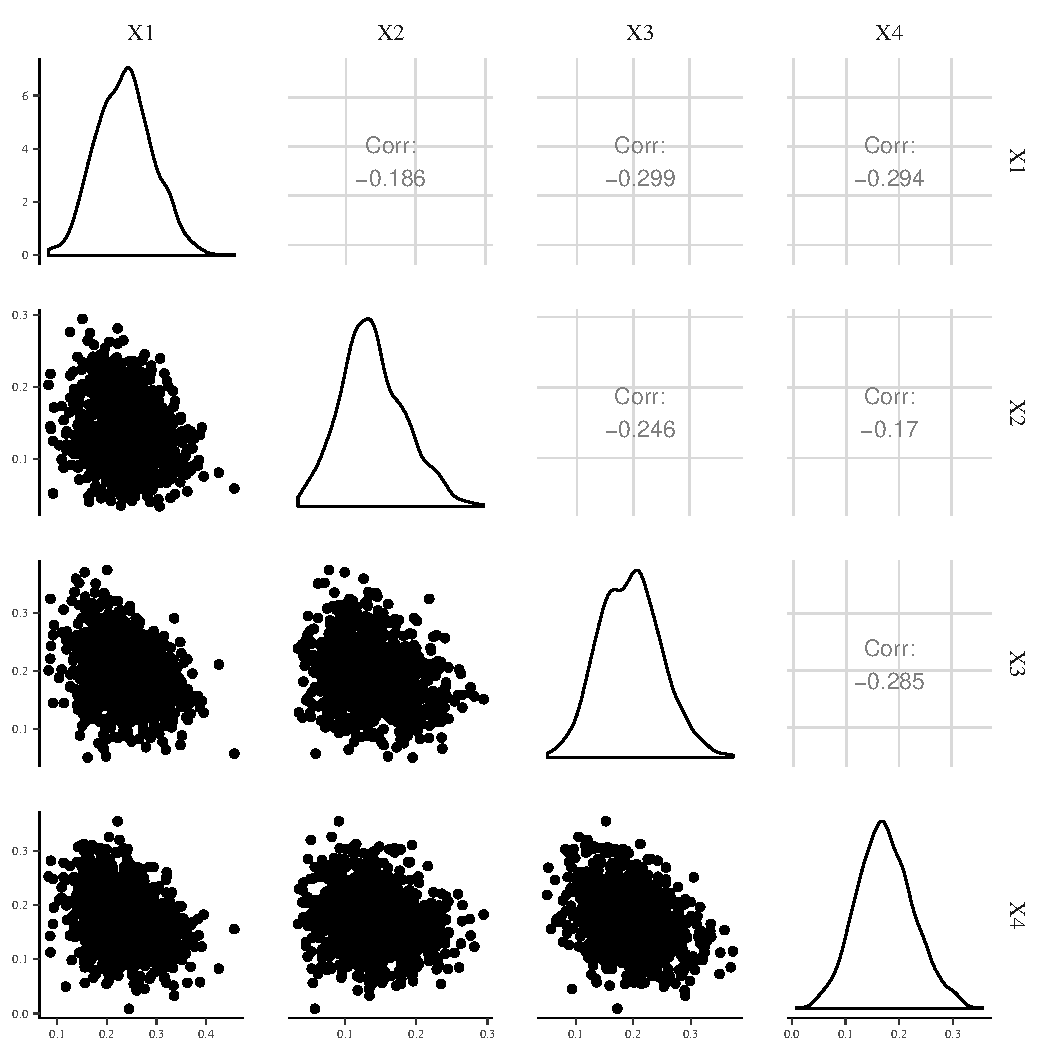
\includegraphics[width=\textwidth-3cm]{figure/ch03_figsimdata_LMG-1} 

}


\begin{kframe}\begin{alltt}
\hlcom{# Comparison to relaimpo package}

\hlstd{fit} \hlkwb{<-} \hlkwd{lm}\hlstd{(y}\hlopt{~}\hlstd{.,} \hlkwc{data}\hlstd{=df)}

\hlcom{######## compare to relimp package}

\hlstd{run}\hlkwb{<-}\hlkwd{boot.relimp}\hlstd{(fit,} \hlkwc{fixed}\hlstd{=}\hlnum{TRUE}\hlstd{)}

\hlkwd{booteval.relimp}\hlstd{(run,} \hlkwc{bty} \hlstd{=} \hlstr{"perc"}\hlstd{,} \hlkwc{level} \hlstd{=} \hlnum{0.95}\hlstd{,}
                \hlkwc{sort} \hlstd{=} \hlnum{FALSE}\hlstd{,} \hlkwc{norank} \hlstd{=} \hlnum{TRUE}\hlstd{,} \hlkwc{nodiff} \hlstd{=} \hlnum{TRUE}\hlstd{,}
                \hlkwc{typesel} \hlstd{=} \hlkwd{c}\hlstd{(}\hlstr{"lmg"}\hlstd{))}
\end{alltt}
\begin{verbatim}
## Response variable: y 
## Total response variance: 4.36 
## Analysis based on 50 observations 
## 
## 4 Regressors: 
## x1 x2 x3 x4 
## Proportion of variance explained by model: 84.8%
## Metrics are not normalized (rela=FALSE). 
## 
## Relative importance metrics: 
## 
##      lmg
## x1 0.167
## x2 0.121
## x3 0.266
## x4 0.294
## 
## Average coefficients for different model sizes: 
## 
##       1X   2Xs   3Xs   4Xs
## x1 0.968 1.004 1.046 1.097
## x2 0.773 0.789 0.815 0.855
## x3 1.160 1.087 0.997 0.882
## x4 1.091 1.106 1.126 1.153
## 
##  
##  Confidence interval information ( 1000 bootstrap replicates, bty= perc ): 
## Relative Contributions with confidence intervals: 
##  
##                   Lower  Upper
##        percentage 0.95   0.95  
## x1.lmg 0.1669     0.0983 0.2576
## x2.lmg 0.1211     0.0631 0.2042
## x3.lmg 0.2659     0.1810 0.3666
## x4.lmg 0.2941     0.2075 0.3899
## 
## CAUTION: Bootstrap confidence intervals can be somewhat liberal. 
## NOTE: X-matrix has been considered as fixed for bootstrapping.
\end{verbatim}
\end{kframe}
\end{knitrout}

\begin{table}[h]
\centering
\begin{tabular}{clll}
  \hline
  \multicolumn{1}{c}{\textbf{Variable}} & \multicolumn{1}{c}{\textbf{I}} &\multicolumn{1}{c}{\textbf{J}} & \multicolumn{1}{c}{\textbf{Total}} \\
  \hline
x1 & 0.164 (0.087, 0.247)  & -0.017 (-0.025, -0.009)   & 0.146 (0.074, 0.227)  \\ 
x2 & 0.119 (0.057, 0.202)  & -0.009 (-0.017, -0.003)   & 0.109 (0.05, 0.191)  \\ 
x3 & 0.258 (0.165, 0.354)  & 0.07 (0.059, 0.078)   & 0.329 (0.224, 0.429)  \\ 
x4 & 0.285 (0.186, 0.383)  & -0.011 (-0.02, \ensuremath{-9.196\times 10^{-4}})   & 0.275 (0.177, 0.373)  \\ 

   \hline
\end{tabular}
\caption{Variance decomposition for stochastic predictors using bootstrap. I = LMG values, J = joint contribution, Total = total explained variance in one-predictor only model}
\label{tbl:fundus.to.SLO}
\end{table}




Using the default uninformative priors, the LMG distributions obtained from the Bayesian framework are very similar to the bootstrap confidence intervals of the LMG estimates obtained from the relaimpo package. In both cases fixed regressors are assumed. In the example above the predictors were sampled from a normal distribution. It would therefore be more reasonable to assume stochastic predictors. As noted in ... under the assumption of weak exogeinity and conditional independence the posterior distributions of the regression paramters $\bbeta$ are valid for fixed and stochastic predictors. Inference about the covariance matrix can be seen as an independent problem. G recommends in most cases to use the non fixed regressor option when calculating bootstrap confidence intervals. The confidence intervals will then in general be a bit larger. If we want to include this uncertainty in the Bayesian framework, we would need some ideas about the distribution of the predictor variables $\X$. It is then possible to obtain poserior distributions of their corresponding covariance matrix. As a practical solution nonparametric bootstrap may be used to include the uncertainty of the covariance matrix. The following code includes the uncertainty of the stochastic predictors. 


\begin{knitrout}
\definecolor{shadecolor}{rgb}{0.98, 0.98, 0.98}\color{fgcolor}\begin{kframe}
\begin{alltt}
\hlcom{#Code assuming stochastic predictors}
\hlstd{run.stochastic}\hlkwb{<-}\hlkwd{boot.relimp}\hlstd{(fit,} \hlkwc{fixed}\hlstd{=}\hlnum{FALSE}\hlstd{)}

\hlkwd{booteval.relimp}\hlstd{(run.stochastic,} \hlkwc{bty} \hlstd{=} \hlstr{"perc"}\hlstd{,} \hlkwc{level} \hlstd{=} \hlnum{0.95}\hlstd{,}
                \hlkwc{sort} \hlstd{=} \hlnum{FALSE}\hlstd{,} \hlkwc{norank} \hlstd{=} \hlnum{TRUE}\hlstd{,} \hlkwc{nodiff} \hlstd{=} \hlnum{TRUE}\hlstd{,}
                \hlkwc{typesel} \hlstd{=} \hlkwd{c}\hlstd{(}\hlstr{"lmg"}\hlstd{))}
\end{alltt}
\begin{verbatim}
## Response variable: y 
## Total response variance: 4.36 
## Analysis based on 50 observations 
## 
## 4 Regressors: 
## x1 x2 x3 x4 
## Proportion of variance explained by model: 84.8%
## Metrics are not normalized (rela=FALSE). 
## 
## Relative importance metrics: 
## 
##      lmg
## x1 0.167
## x2 0.121
## x3 0.266
## x4 0.294
## 
## Average coefficients for different model sizes: 
## 
##       1X   2Xs   3Xs   4Xs
## x1 0.968 1.004 1.046 1.097
## x2 0.773 0.789 0.815 0.855
## x3 1.160 1.087 0.997 0.882
## x4 1.091 1.106 1.126 1.153
## 
##  
##  Confidence interval information ( 1000 bootstrap replicates, bty= perc ): 
## Relative Contributions with confidence intervals: 
##  
##                   Lower  Upper
##        percentage 0.95   0.95  
## x1.lmg 0.1669     0.0883 0.2838
## x2.lmg 0.1211     0.0468 0.2353
## x3.lmg 0.2659     0.1346 0.4001
## x4.lmg 0.2941     0.1493 0.4099
## 
## CAUTION: Bootstrap confidence intervals can be somewhat liberal.
\end{verbatim}
\begin{alltt}
\hlcom{#----------------------------------------------------------------------------------------}


\hlstd{df.rtwos.boot} \hlkwb{<-}\hlkwd{rtwos.boot}\hlstd{(df[,}\hlnum{2}\hlopt{:}\hlnum{5}\hlstd{], post.sample,} \hlnum{100}\hlstd{)}

\hlstd{n.boot} \hlkwb{=} \hlnum{100}

\hlstd{LMG.Vals.I.boot}\hlkwb{<-}\hlkwd{array}\hlstd{(}\hlnum{0}\hlstd{,} \hlkwd{c}\hlstd{(}\hlnum{4}\hlstd{,}\hlkwd{dim}\hlstd{(df.rtwos.boot)[}\hlnum{2}\hlstd{], n.boot))}
\hlstd{LMG.Vals.J.boot}\hlkwb{<-}\hlkwd{array}\hlstd{(}\hlnum{0}\hlstd{,} \hlkwd{c}\hlstd{(}\hlnum{4}\hlstd{,}\hlkwd{dim}\hlstd{(df.rtwos.boot)[}\hlnum{2}\hlstd{], n.boot))}
\hlstd{LMG.Vals.T.boot}\hlkwb{<-}\hlkwd{array}\hlstd{(}\hlnum{0}\hlstd{,} \hlkwd{c}\hlstd{(}\hlnum{4}\hlstd{,}\hlkwd{dim}\hlstd{(df.rtwos.boot)[}\hlnum{2}\hlstd{], n.boot))}

\hlkwa{for} \hlstd{(b} \hlkwa{in} \hlnum{1}\hlopt{:}\hlstd{n.boot)\{}

\hlkwa{for}\hlstd{(i} \hlkwa{in} \hlnum{1}\hlopt{:}\hlkwd{dim}\hlstd{(df.rtwos.boot)[}\hlnum{2}\hlstd{])\{}

        \hlstd{gofn}\hlkwb{<-}\hlstd{df.rtwos.boot[,i,b]}

        \hlstd{obj.Gelman}\hlkwb{<-}\hlkwd{partition}\hlstd{(gofn,} \hlkwc{pcan} \hlstd{=} \hlnum{4}\hlstd{,} \hlkwc{var.names} \hlstd{=} \hlkwd{names}\hlstd{(df[,}\hlnum{2}\hlopt{:}\hlnum{5}\hlstd{]))}

        \hlstd{LMG.Vals.I.boot[,i, b]}\hlkwb{=}\hlstd{obj.Gelman}\hlopt{$}\hlstd{IJ[,}\hlnum{1}\hlstd{]}
        \hlstd{LMG.Vals.J.boot[,i, b]}\hlkwb{=}\hlstd{obj.Gelman}\hlopt{$}\hlstd{IJ[,}\hlnum{2}\hlstd{]}
        \hlstd{LMG.Vals.T.boot[,i, b]}\hlkwb{=}\hlstd{obj.Gelman}\hlopt{$}\hlstd{IJ[,}\hlnum{3}\hlstd{]}

\hlstd{\}}

\hlstd{\}}

\hlkwd{quantile}\hlstd{(}\hlkwd{c}\hlstd{(LMG.Vals.I.boot[}\hlnum{1}\hlstd{,}\hlnum{1}\hlopt{:}\hlnum{1000}\hlstd{,]),} \hlkwd{c}\hlstd{(}\hlnum{0.025}\hlstd{,} \hlnum{0.5}\hlstd{,} \hlnum{0.975}\hlstd{))}
\end{alltt}
\begin{verbatim}
##   2.5%    50%  97.5% 
## 0.0724 0.1652 0.2766
\end{verbatim}
\begin{alltt}
\hlkwd{quantile}\hlstd{(}\hlkwd{c}\hlstd{(LMG.Vals.I.boot[}\hlnum{2}\hlstd{,}\hlnum{1}\hlopt{:}\hlnum{1000}\hlstd{,]),} \hlkwd{c}\hlstd{(}\hlnum{0.025}\hlstd{,} \hlnum{0.5}\hlstd{,} \hlnum{0.975}\hlstd{))}
\end{alltt}
\begin{verbatim}
##   2.5%    50%  97.5% 
## 0.0369 0.1142 0.2263
\end{verbatim}
\begin{alltt}
\hlkwd{quantile}\hlstd{(}\hlkwd{c}\hlstd{(LMG.Vals.I.boot[}\hlnum{3}\hlstd{,}\hlnum{1}\hlopt{:}\hlnum{1000}\hlstd{,]),} \hlkwd{c}\hlstd{(}\hlnum{0.025}\hlstd{,} \hlnum{0.5}\hlstd{,} \hlnum{0.975}\hlstd{))}
\end{alltt}
\begin{verbatim}
##  2.5%   50% 97.5% 
## 0.140 0.261 0.380
\end{verbatim}
\begin{alltt}
\hlkwd{quantile}\hlstd{(}\hlkwd{c}\hlstd{(LMG.Vals.I.boot[}\hlnum{4}\hlstd{,}\hlnum{1}\hlopt{:}\hlnum{1000}\hlstd{,]),} \hlkwd{c}\hlstd{(}\hlnum{0.025}\hlstd{,} \hlnum{0.5}\hlstd{,} \hlnum{0.975}\hlstd{))}
\end{alltt}
\begin{verbatim}
##  2.5%   50% 97.5% 
## 0.154 0.278 0.408
\end{verbatim}
\begin{alltt}
\hlcom{#very similar values as in the confidence intervals for stochastic predictors}


\hlcom{#what if we have prior knowledge}
\hlstd{my_prior} \hlkwb{<-} \hlkwd{normal}\hlstd{(}\hlkwc{location} \hlstd{=} \hlkwd{c}\hlstd{(}\hlnum{1}\hlstd{,} \hlnum{1}\hlstd{,}\hlnum{1}\hlstd{,}\hlnum{1}\hlstd{),} \hlkwc{scale} \hlstd{=} \hlkwd{c}\hlstd{(}\hlnum{0.01}\hlstd{,} \hlnum{0.01}\hlstd{,}\hlnum{0.01}\hlstd{,}\hlnum{0.01}\hlstd{),} \hlkwc{autoscale} \hlstd{=} \hlnum{FALSE}\hlstd{)}

\hlstd{post2} \hlkwb{<-} \hlkwd{stan_glm}\hlstd{(y} \hlopt{~} \hlnum{1} \hlopt{+} \hlstd{x1} \hlopt{+} \hlstd{x2} \hlopt{+} \hlstd{x3} \hlopt{+} \hlstd{x4,}
                  \hlkwc{data} \hlstd{= df,} \hlkwc{prior} \hlstd{= my_prior,}
                  \hlkwc{chains} \hlstd{=} \hlnum{2}\hlstd{,} \hlkwc{cores} \hlstd{=} \hlnum{1}\hlstd{)}
\end{alltt}
\begin{verbatim}
## 
## SAMPLING FOR MODEL 'continuous' NOW (CHAIN 1).
## 
## Gradient evaluation took 2.6e-05 seconds
## 1000 transitions using 10 leapfrog steps per transition would take 0.26 seconds.
## Adjust your expectations accordingly!
## 
## 
## Iteration:    1 / 2000 [  0%]  (Warmup)
## Iteration:  200 / 2000 [ 10%]  (Warmup)
## Iteration:  400 / 2000 [ 20%]  (Warmup)
## Iteration:  600 / 2000 [ 30%]  (Warmup)
## Iteration:  800 / 2000 [ 40%]  (Warmup)
## Iteration: 1000 / 2000 [ 50%]  (Warmup)
## Iteration: 1001 / 2000 [ 50%]  (Sampling)
## Iteration: 1200 / 2000 [ 60%]  (Sampling)
## Iteration: 1400 / 2000 [ 70%]  (Sampling)
## Iteration: 1600 / 2000 [ 80%]  (Sampling)
## Iteration: 1800 / 2000 [ 90%]  (Sampling)
## Iteration: 2000 / 2000 [100%]  (Sampling)
## 
##  Elapsed Time: 0.087333 seconds (Warm-up)
##                0.064388 seconds (Sampling)
##                0.151721 seconds (Total)
## 
## 
## SAMPLING FOR MODEL 'continuous' NOW (CHAIN 2).
## 
## Gradient evaluation took 1.5e-05 seconds
## 1000 transitions using 10 leapfrog steps per transition would take 0.15 seconds.
## Adjust your expectations accordingly!
## 
## 
## Iteration:    1 / 2000 [  0%]  (Warmup)
## Iteration:  200 / 2000 [ 10%]  (Warmup)
## Iteration:  400 / 2000 [ 20%]  (Warmup)
## Iteration:  600 / 2000 [ 30%]  (Warmup)
## Iteration:  800 / 2000 [ 40%]  (Warmup)
## Iteration: 1000 / 2000 [ 50%]  (Warmup)
## Iteration: 1001 / 2000 [ 50%]  (Sampling)
## Iteration: 1200 / 2000 [ 60%]  (Sampling)
## Iteration: 1400 / 2000 [ 70%]  (Sampling)
## Iteration: 1600 / 2000 [ 80%]  (Sampling)
## Iteration: 1800 / 2000 [ 90%]  (Sampling)
## Iteration: 2000 / 2000 [100%]  (Sampling)
## 
##  Elapsed Time: 0.089243 seconds (Warm-up)
##                0.063377 seconds (Sampling)
##                0.15262 seconds (Total)
\end{verbatim}
\begin{alltt}
\hlcom{#posterior sample}
\hlstd{post.sample} \hlkwb{<-} \hlkwd{as.matrix}\hlstd{(post2)}

\hlcom{#example of the first 10 posterior samples}
\hlstd{post.sample[}\hlnum{1}\hlopt{:}\hlnum{10}\hlstd{,]}
\end{alltt}
\begin{verbatim}
##           parameters
## iterations (Intercept)    x1    x2    x3    x4 sigma
##       [1,]      0.0626 0.988 0.999 1.005 0.997 0.766
##       [2,]      0.1738 1.009 1.006 0.995 1.002 0.853
##       [3,]     -0.0564 0.993 0.990 1.012 0.993 0.926
##       [4,]     -0.1099 0.997 0.999 1.018 0.998 1.143
##       [5,]      0.1825 1.003 0.998 0.979 1.004 0.759
##       [6,]     -0.1708 0.999 1.017 1.009 1.000 0.906
##       [7,]      0.1113 1.006 1.000 0.990 0.991 0.770
##       [8,]     -0.0681 0.991 1.001 1.008 1.011 0.952
##       [9,]      0.0660 1.010 0.995 0.989 1.011 0.764
##      [10,]     -0.0335 0.991 1.004 1.010 0.991 0.938
\end{verbatim}
\begin{alltt}
\hlcom{#no need for the intercept, last parameter is sigma}
\hlstd{post.sample} \hlkwb{<-} \hlstd{post.sample[,}\hlopt{-}\hlnum{1}\hlstd{]}


\hlcom{#data frame with all submodels}


\hlstd{df.rtwos.boot} \hlkwb{<-}\hlkwd{rtwos.boot}\hlstd{(df[,}\hlnum{2}\hlopt{:}\hlnum{5}\hlstd{], post.sample,} \hlnum{10}\hlstd{)}

\hlstd{n.boot} \hlkwb{=} \hlnum{10}

\hlstd{LMG.Vals.I.boot.p}\hlkwb{<-}\hlkwd{array}\hlstd{(}\hlnum{0}\hlstd{,} \hlkwd{c}\hlstd{(}\hlnum{4}\hlstd{,}\hlkwd{dim}\hlstd{(df.rtwos.boot)[}\hlnum{2}\hlstd{], n.boot))}

\hlkwa{for} \hlstd{(b} \hlkwa{in} \hlnum{1}\hlopt{:}\hlstd{n.boot)\{}

\hlkwa{for}\hlstd{(i} \hlkwa{in} \hlnum{1}\hlopt{:}\hlkwd{dim}\hlstd{(df.rtwos.boot)[}\hlnum{2}\hlstd{])\{}

        \hlstd{gofn}\hlkwb{<-}\hlstd{df.rtwos.boot[,i,b]}

        \hlstd{obj.Gelman}\hlkwb{<-}\hlkwd{partition}\hlstd{(gofn,} \hlkwc{pcan} \hlstd{=} \hlnum{4}\hlstd{,} \hlkwc{var.names} \hlstd{=} \hlkwd{names}\hlstd{(df[,}\hlnum{2}\hlopt{:}\hlnum{5}\hlstd{]))}

        \hlstd{LMG.Vals.I.boot.p[,i, b]}\hlkwb{=}\hlstd{obj.Gelman}\hlopt{$}\hlstd{IJ[,}\hlnum{1}\hlstd{]}
\hlstd{\}}

\hlstd{\}}

\hlkwd{quantile}\hlstd{(}\hlkwd{c}\hlstd{(LMG.Vals.I.boot.p[}\hlnum{1}\hlstd{,}\hlnum{1}\hlopt{:}\hlnum{1000}\hlstd{,]),} \hlkwd{c}\hlstd{(}\hlnum{0.025}\hlstd{,} \hlnum{0.5}\hlstd{,} \hlnum{0.975}\hlstd{))}
\end{alltt}
\begin{verbatim}
##   2.5%    50%  97.5% 
## 0.0798 0.1373 0.1899
\end{verbatim}
\begin{alltt}
\hlkwd{quantile}\hlstd{(}\hlkwd{c}\hlstd{(LMG.Vals.I.boot.p[}\hlnum{2}\hlstd{,}\hlnum{1}\hlopt{:}\hlnum{1000}\hlstd{,]),} \hlkwd{c}\hlstd{(}\hlnum{0.025}\hlstd{,} \hlnum{0.5}\hlstd{,} \hlnum{0.975}\hlstd{))}
\end{alltt}
\begin{verbatim}
##  2.5%   50% 97.5% 
## 0.105 0.177 0.217
\end{verbatim}
\begin{alltt}
\hlkwd{quantile}\hlstd{(}\hlkwd{c}\hlstd{(LMG.Vals.I.boot.p[}\hlnum{3}\hlstd{,}\hlnum{1}\hlopt{:}\hlnum{1000}\hlstd{,]),} \hlkwd{c}\hlstd{(}\hlnum{0.025}\hlstd{,} \hlnum{0.5}\hlstd{,} \hlnum{0.975}\hlstd{))}
\end{alltt}
\begin{verbatim}
##  2.5%   50% 97.5% 
## 0.277 0.324 0.380
\end{verbatim}
\begin{alltt}
\hlkwd{quantile}\hlstd{(}\hlkwd{c}\hlstd{(LMG.Vals.I.boot.p[}\hlnum{4}\hlstd{,}\hlnum{1}\hlopt{:}\hlnum{1000}\hlstd{,]),} \hlkwd{c}\hlstd{(}\hlnum{0.025}\hlstd{,} \hlnum{0.5}\hlstd{,} \hlnum{0.975}\hlstd{))}
\end{alltt}
\begin{verbatim}
##  2.5%   50% 97.5% 
## 0.161 0.213 0.269
\end{verbatim}
\end{kframe}
\end{knitrout}



\begin{table}[h]
\centering
\begin{tabular}{clll}
  \hline
  \multicolumn{1}{c}{\textbf{Variable}} & \multicolumn{1}{c}{\textbf{I}} &\multicolumn{1}{c}{\textbf{J}} & \multicolumn{1}{c}{\textbf{Total}} \\
  \hline
x1 & 0.165 (0.072, 0.277)  & -0.01 (-0.08, 0.1)   & 0.154 (0.03, 0.326)  \\ 
x2 & 0.114 (0.037, 0.226)  & -0.014 (-0.063, 0.078)   & 0.102 (0.005, 0.268)  \\ 
x3 & 0.261 (0.14, 0.38)  & 0.073 (-0.026, 0.207)   & 0.336 (0.145, 0.536)  \\ 
x4 & 0.278 (0.154, 0.408)  & -0.007 (-0.093, 0.133)   & 0.274 (0.095, 0.474)  \\ 

   \hline
\end{tabular}
\caption{Variance decomposition. I = LMG values, J = joint contribution, Total = total explained variance in one-predictor only model}
\label{tbl:fundus.to.SLO2}
\end{table}




In the following example we know that the $\X$ are coming from a normal distribution. The covariance matrix of the distribution is estimated in a Bayesian way. The package Jags is used.

\begin{knitrout}
\definecolor{shadecolor}{rgb}{0.98, 0.98, 0.98}\color{fgcolor}\begin{kframe}
\begin{alltt}
\hlstd{zy} \hlkwb{=} \hlstd{df[,}\hlnum{2}\hlopt{:}\hlnum{5}\hlstd{]}

\hlcom{#----------------------------------------------------------------------------}
\hlcom{# The rest can remain unchanged, except for the specification of difference of}
\hlcom{# correlations at the very end.}
\hlcom{#----------------------------------------------------------------------------}

\hlcom{# Load some functions used below:}
\hlcom{# Install the ellipse package if not already:}
\hlcom{# Standardize the data:}

\hlcom{#zy = apply(y,2,function(yVec)\{(yVec-mean(yVec))/sd(yVec)\})}
\hlcom{# Assemble data for sending to JAGS:}
\hlstd{dataList} \hlkwb{=} \hlkwd{list}\hlstd{(}
        \hlkwc{zy} \hlstd{= zy ,}
        \hlkwc{Ntotal} \hlstd{=}  \hlkwd{nrow}\hlstd{(zy) ,}
        \hlkwc{Nvar} \hlstd{=} \hlkwd{ncol}\hlstd{(zy) ,}
        \hlcom{# Include original data info for transforming to original scale:}
        \hlcom{# For wishart (dwish) prior on inverse covariance matrix:}
        \hlkwc{zRscal} \hlstd{=} \hlkwd{ncol}\hlstd{(zy) ,}  \hlcom{# for dwish prior}
        \hlkwc{zRmat} \hlstd{=} \hlkwd{diag}\hlstd{(}\hlkwc{x}\hlstd{=}\hlnum{1}\hlstd{,}\hlkwc{nrow}\hlstd{=}\hlkwd{ncol}\hlstd{(zy))}  \hlcom{# Rmat = diag(apply(y,2,var))}
\hlstd{)}

\hlcom{# Define the model:}
\hlstd{modelString} \hlkwb{=} \hlstr{"
model \{
for ( i in 1:Ntotal ) \{
zy[i,1:Nvar] ~ dmnorm( zMu[1:Nvar] , zInvCovMat[1:Nvar,1:Nvar] ) 
\}
for ( varIdx in 1:Nvar ) \{ zMu[varIdx] ~ dnorm( 0 , 1/2^2 ) \}
zInvCovMat ~ dwish( zRmat[1:Nvar,1:Nvar] , zRscal )
# Convert invCovMat to sd and correlation:
zCovMat <- inverse( zInvCovMat )

\}
"} \hlcom{# close quote for modelString}
\hlkwd{writeLines}\hlstd{( modelString ,} \hlkwc{con}\hlstd{=}\hlstr{"Jags-MultivariateNormal-model.txt"} \hlstd{)}

\hlcom{# Run the chains:}
\hlstd{nChain} \hlkwb{=} \hlnum{3}
\hlstd{nAdapt} \hlkwb{=} \hlnum{500}
\hlstd{nBurnIn} \hlkwb{=} \hlnum{500}
\hlstd{nThin} \hlkwb{=} \hlnum{10}
\hlstd{nStepToSave} \hlkwb{=} \hlnum{20000}
\hlkwd{require}\hlstd{(rjags)}
\hlstd{jagsModel} \hlkwb{=} \hlkwd{jags.model}\hlstd{(} \hlkwc{file}\hlstd{=}\hlstr{"Jags-MultivariateNormal-model.txt"} \hlstd{,}
                                                                                                \hlkwc{data}\hlstd{=dataList ,} \hlkwc{n.chains}\hlstd{=nChain ,} \hlkwc{n.adapt}\hlstd{=nAdapt )}
\end{alltt}
\begin{verbatim}
## Compiling model graph
##    Resolving undeclared variables
##    Allocating nodes
## Graph information:
##    Observed stochastic nodes: 50
##    Unobserved stochastic nodes: 5
##    Total graph size: 82
## 
## Initializing model
\end{verbatim}
\begin{alltt}
\hlkwd{update}\hlstd{( jagsModel ,} \hlkwc{n.iter}\hlstd{=nBurnIn )}
\hlstd{codaSamples} \hlkwb{=} \hlkwd{coda.samples}\hlstd{( jagsModel ,}
                                                                                                                \hlkwc{variable.names}\hlstd{=}\hlkwd{c}\hlstd{(}\hlstr{'zCovMat'}\hlstd{) ,}
                                                                                                                \hlkwc{n.iter}\hlstd{=nStepToSave}\hlopt{/}\hlstd{nChain}\hlopt{*}\hlstd{nThin ,} \hlkwc{thin}\hlstd{=nThin )}


\hlcom{# Convergence diagnostics:}
\hlstd{parameterNames} \hlkwb{=} \hlkwd{varnames}\hlstd{(codaSamples)} \hlcom{# get all parameter names}


\hlcom{# Examine the posterior distribution:}
\hlstd{mcmcMat} \hlkwb{=} \hlkwd{as.matrix}\hlstd{(codaSamples)}
\hlstd{chainLength} \hlkwb{=} \hlkwd{nrow}\hlstd{(mcmcMat)}

\hlstd{covMat} \hlkwb{<-} \hlkwd{array}\hlstd{(}\hlnum{NA}\hlstd{,} \hlkwd{c}\hlstd{(}\hlnum{4}\hlstd{,}\hlnum{4}\hlstd{,chainLength))}

\hlkwa{for} \hlstd{(i} \hlkwa{in} \hlnum{1}\hlopt{:}\hlstd{chainLength)\{}
\hlstd{covMat[}\hlnum{1}\hlopt{:}\hlnum{4}\hlstd{,}\hlnum{1}\hlopt{:}\hlnum{4}\hlstd{,i]}\hlkwb{<-}\hlkwd{matrix}\hlstd{(mcmcMat[i,],} \hlnum{4}\hlstd{,} \hlnum{4}\hlstd{)}
\hlstd{\}}

\hlstd{covMat} \hlkwb{<-} \hlstd{covMat[}\hlnum{1}\hlopt{:}\hlnum{4}\hlstd{,}\hlnum{1}\hlopt{:}\hlnum{4}\hlstd{,}\hlkwd{sample}\hlstd{(}\hlnum{1}\hlopt{:}\hlnum{20000}\hlstd{,} \hlkwc{replace}\hlstd{=F)]}


\hlstd{df.rtwos} \hlkwb{<-}\hlkwd{rtwos.covm}\hlstd{(df[,}\hlnum{2}\hlopt{:}\hlnum{5}\hlstd{], post.sample, covMat,} \hlnum{10}\hlstd{)}


\hlstd{n.boot} \hlkwb{=} \hlnum{10}

\hlstd{LMG.Vals.I.covm}\hlkwb{<-}\hlkwd{array}\hlstd{(}\hlnum{0}\hlstd{,} \hlkwd{c}\hlstd{(}\hlnum{4}\hlstd{,}\hlkwd{dim}\hlstd{(df.rtwos)[}\hlnum{2}\hlstd{], n.boot))}
\hlstd{LMG.Vals.J.covm}\hlkwb{<-}\hlkwd{array}\hlstd{(}\hlnum{0}\hlstd{,} \hlkwd{c}\hlstd{(}\hlnum{4}\hlstd{,}\hlkwd{dim}\hlstd{(df.rtwos.boot)[}\hlnum{2}\hlstd{], n.boot))}
\hlstd{LMG.Vals.T.covm}\hlkwb{<-}\hlkwd{array}\hlstd{(}\hlnum{0}\hlstd{,} \hlkwd{c}\hlstd{(}\hlnum{4}\hlstd{,}\hlkwd{dim}\hlstd{(df.rtwos.boot)[}\hlnum{2}\hlstd{], n.boot))}


\hlkwa{for} \hlstd{(b} \hlkwa{in} \hlnum{1}\hlopt{:}\hlstd{n.boot)\{}

        \hlkwa{for}\hlstd{(i} \hlkwa{in} \hlnum{1}\hlopt{:}\hlkwd{dim}\hlstd{(df.rtwos)[}\hlnum{2}\hlstd{])\{}

                \hlstd{gofn}\hlkwb{<-}\hlstd{df.rtwos[,i,b]}

                \hlstd{obj.Gelman}\hlkwb{<-}\hlkwd{partition}\hlstd{(gofn,} \hlkwc{pcan} \hlstd{=} \hlnum{4}\hlstd{,} \hlkwc{var.names} \hlstd{=} \hlkwd{names}\hlstd{(df[,}\hlnum{2}\hlopt{:}\hlnum{5}\hlstd{]))}

                \hlstd{LMG.Vals.I.covm[,i, b]}\hlkwb{=}\hlstd{obj.Gelman}\hlopt{$}\hlstd{IJ[,}\hlnum{1}\hlstd{]}
                \hlstd{LMG.Vals.J.covm[,i, b]}\hlkwb{=}\hlstd{obj.Gelman}\hlopt{$}\hlstd{IJ[,}\hlnum{2}\hlstd{]}
                \hlstd{LMG.Vals.T.covm[,i, b]}\hlkwb{=}\hlstd{obj.Gelman}\hlopt{$}\hlstd{IJ[,}\hlnum{3}\hlstd{]}

        \hlstd{\}}

\hlstd{\}}

\hlkwd{quantile}\hlstd{(}\hlkwd{c}\hlstd{(LMG.Vals.I.covm[}\hlnum{1}\hlstd{,}\hlnum{1}\hlopt{:}\hlnum{1000}\hlstd{,]),} \hlkwd{c}\hlstd{(}\hlnum{0.025}\hlstd{,} \hlnum{0.5}\hlstd{,} \hlnum{0.975}\hlstd{))}
\end{alltt}
\begin{verbatim}
##   2.5%    50%  97.5% 
## 0.0893 0.1507 0.2076
\end{verbatim}
\begin{alltt}
\hlkwd{quantile}\hlstd{(}\hlkwd{c}\hlstd{(LMG.Vals.I.covm[}\hlnum{2}\hlstd{,}\hlnum{1}\hlopt{:}\hlnum{1000}\hlstd{,]),} \hlkwd{c}\hlstd{(}\hlnum{0.025}\hlstd{,} \hlnum{0.5}\hlstd{,} \hlnum{0.975}\hlstd{))}
\end{alltt}
\begin{verbatim}
##  2.5%   50% 97.5% 
## 0.104 0.141 0.222
\end{verbatim}
\begin{alltt}
\hlkwd{quantile}\hlstd{(}\hlkwd{c}\hlstd{(LMG.Vals.I.covm[}\hlnum{3}\hlstd{,}\hlnum{1}\hlopt{:}\hlnum{1000}\hlstd{,]),} \hlkwd{c}\hlstd{(}\hlnum{0.025}\hlstd{,} \hlnum{0.5}\hlstd{,} \hlnum{0.975}\hlstd{))}
\end{alltt}
\begin{verbatim}
##  2.5%   50% 97.5% 
## 0.264 0.305 0.452
\end{verbatim}
\begin{alltt}
\hlkwd{quantile}\hlstd{(}\hlkwd{c}\hlstd{(LMG.Vals.I.covm[}\hlnum{4}\hlstd{,}\hlnum{1}\hlopt{:}\hlnum{1000}\hlstd{,]),} \hlkwd{c}\hlstd{(}\hlnum{0.025}\hlstd{,} \hlnum{0.5}\hlstd{,} \hlnum{0.975}\hlstd{))}
\end{alltt}
\begin{verbatim}
##  2.5%   50% 97.5% 
## 0.141 0.204 0.315
\end{verbatim}
\end{kframe}
\end{knitrout}


\begin{table}[h]
\centering
\begin{tabular}{clll}
  \hline
  \multicolumn{1}{c}{\textbf{Variable}} & \multicolumn{1}{c}{\textbf{I}} &\multicolumn{1}{c}{\textbf{J}} & \multicolumn{1}{c}{\textbf{Total}} \\
  \hline
x1 & 0.151 (0.089, 0.208)  & 0.016 (-0.063, 0.114)   & 0.173 (0.03, 0.322)  \\ 
x2 & 0.141 (0.104, 0.222)  & -0.008 (-0.091, 0.04)   & 0.137 (0.038, 0.246)  \\ 
x3 & 0.305 (0.264, 0.452)  & 0.118 (0.04, 0.167)   & 0.432 (0.32, 0.564)  \\ 
x4 & 0.204 (0.141, 0.315)  & 0.019 (-0.047, 0.133)   & 0.22 (0.096, 0.448)  \\ 

   \hline
\end{tabular}
\caption{Variance decomposition. I = LMG values, J = joint contribution, Total = total explained variance in one-predictor only model}
\label{tbl:fundus.to.SLO3}
\end{table}

Using the bootstrap samples of the covariance matrix or samples from the posterior covariance matrix resulted in very similar LMG values. Bootstrap seems to be a valuable option for stochastic predictors when the distribution of the predictors is unknown. Even when the distribution is known the difference seems to be tiny. A benefit of going the full Bayesian way is that we can also include prior knowledge of the covariance matrix. For stochastic predictors the uncertainty about the covariance matrix is reflected in the large credible intervals. Even when we would knew the exact regression parameters, there is alot of uncertainty in the LMG values caused by the uncertainty about the covariance matrix. Code xx shows the uncertainty about the LMG values caused by the uncertainty about the covariance matrix. 

Another interesting option in some cases would be to use the shrinkage estimate of the covariance matrix. 


\begin{knitrout}
\definecolor{shadecolor}{rgb}{0.98, 0.98, 0.98}\color{fgcolor}\begin{kframe}
\begin{alltt}
\hlcom{#How much variance is effectively in the bootstrap matrix when we know the regression parameters.}

\hlcom{#fake post sample}

\hlstd{x1} \hlkwb{<-} \hlkwd{rnorm}\hlstd{(}\hlnum{50}\hlstd{,} \hlnum{0}\hlstd{,} \hlnum{1}\hlstd{); x2} \hlkwb{<-} \hlkwd{rnorm}\hlstd{(}\hlnum{50}\hlstd{,} \hlnum{0}\hlstd{,} \hlnum{1}\hlstd{)}
\hlstd{x3} \hlkwb{<-} \hlkwd{rnorm}\hlstd{(}\hlnum{50}\hlstd{,} \hlnum{0}\hlstd{,} \hlnum{1}\hlstd{); x4} \hlkwb{<-} \hlkwd{rnorm}\hlstd{(}\hlnum{50}\hlstd{,} \hlnum{0}\hlstd{,} \hlnum{1}\hlstd{)}
\hlcom{#b1 <- 0.5; b2 <- 1; b3 <- 2; b4 <- 0}
\hlstd{b1} \hlkwb{<-} \hlnum{1}\hlstd{; b2} \hlkwb{<-} \hlnum{1}\hlstd{; b3} \hlkwb{<-} \hlnum{1}\hlstd{; b4} \hlkwb{<-} \hlnum{1}

\hlstd{y} \hlkwb{<-} \hlstd{b1}\hlopt{*}\hlstd{x1} \hlopt{+} \hlstd{x2}\hlopt{*}\hlstd{b2} \hlopt{+} \hlstd{b3}\hlopt{*}\hlstd{x3} \hlopt{+} \hlstd{b4}\hlopt{*}\hlstd{x4} \hlopt{+} \hlkwd{rnorm}\hlstd{(}\hlnum{50}\hlstd{,} \hlnum{0}\hlstd{,} \hlnum{1}\hlstd{)}

\hlstd{df} \hlkwb{<-} \hlkwd{data.frame}\hlstd{(}\hlkwc{y} \hlstd{= y,} \hlkwc{x1} \hlstd{= x1,} \hlkwc{x2} \hlstd{= x2,} \hlkwc{x3} \hlstd{= x3,} \hlkwc{x4} \hlstd{= x4)}

\hlstd{post.sample} \hlkwb{<-} \hlkwd{matrix}\hlstd{(}\hlnum{1}\hlstd{,} \hlnum{1}\hlstd{,}\hlnum{5}\hlstd{)}

\hlstd{df.rtwos.boot} \hlkwb{<-}\hlkwd{rtwos.boot}\hlstd{(df[,}\hlnum{2}\hlopt{:}\hlnum{5}\hlstd{], post.sample,} \hlnum{1000}\hlstd{)}

\hlstd{n.boot} \hlkwb{=} \hlnum{1000}

\hlstd{LMG.Vals.I.boot}\hlkwb{<-}\hlkwd{array}\hlstd{(}\hlnum{0}\hlstd{,} \hlkwd{c}\hlstd{(}\hlnum{4}\hlstd{,}\hlkwd{dim}\hlstd{(df.rtwos.boot)[}\hlnum{2}\hlstd{], n.boot))}

\hlkwa{for} \hlstd{(b} \hlkwa{in} \hlnum{1}\hlopt{:}\hlstd{n.boot)\{}

\hlkwa{for}\hlstd{(i} \hlkwa{in} \hlnum{1}\hlopt{:}\hlkwd{dim}\hlstd{(df.rtwos.boot)[}\hlnum{2}\hlstd{])\{}

        \hlstd{gofn}\hlkwb{<-}\hlstd{df.rtwos.boot[,i,b]}

        \hlstd{obj.Gelman}\hlkwb{<-}\hlkwd{partition}\hlstd{(gofn,} \hlkwc{pcan} \hlstd{=} \hlnum{4}\hlstd{,} \hlkwc{var.names} \hlstd{=} \hlkwd{names}\hlstd{(df[,}\hlnum{2}\hlopt{:}\hlnum{5}\hlstd{]))}

        \hlstd{LMG.Vals.I.boot[,i, b]}\hlkwb{=}\hlstd{obj.Gelman}\hlopt{$}\hlstd{IJ[,}\hlnum{1}\hlstd{]}
\hlstd{\}}

\hlstd{\}}

\hlkwd{quantile}\hlstd{(}\hlkwd{c}\hlstd{(LMG.Vals.I.boot[}\hlnum{1}\hlstd{,}\hlnum{1}\hlstd{,]),} \hlkwd{c}\hlstd{(}\hlnum{0.025}\hlstd{,} \hlnum{0.5}\hlstd{,} \hlnum{0.975}\hlstd{))}
\end{alltt}
\begin{verbatim}
##   2.5%    50%  97.5% 
## 0.0809 0.1493 0.2391
\end{verbatim}
\begin{alltt}
\hlkwd{quantile}\hlstd{(}\hlkwd{c}\hlstd{(LMG.Vals.I.boot[}\hlnum{2}\hlstd{,}\hlnum{1}\hlstd{,]),} \hlkwd{c}\hlstd{(}\hlnum{0.025}\hlstd{,} \hlnum{0.5}\hlstd{,} \hlnum{0.975}\hlstd{))}
\end{alltt}
\begin{verbatim}
##  2.5%   50% 97.5% 
## 0.162 0.252 0.334
\end{verbatim}
\begin{alltt}
\hlkwd{quantile}\hlstd{(}\hlkwd{c}\hlstd{(LMG.Vals.I.boot[}\hlnum{3}\hlstd{,}\hlnum{1}\hlstd{,]),} \hlkwd{c}\hlstd{(}\hlnum{0.025}\hlstd{,} \hlnum{0.5}\hlstd{,} \hlnum{0.975}\hlstd{))}
\end{alltt}
\begin{verbatim}
##   2.5%    50%  97.5% 
## 0.0944 0.1888 0.2925
\end{verbatim}
\begin{alltt}
\hlkwd{quantile}\hlstd{(}\hlkwd{c}\hlstd{(LMG.Vals.I.boot[}\hlnum{4}\hlstd{,}\hlnum{1}\hlstd{,]),} \hlkwd{c}\hlstd{(}\hlnum{0.025}\hlstd{,} \hlnum{0.5}\hlstd{,} \hlnum{0.975}\hlstd{))}
\end{alltt}
\begin{verbatim}
##  2.5%   50% 97.5% 
## 0.137 0.245 0.347
\end{verbatim}
\begin{alltt}
\hlstd{dat} \hlkwb{<-} \hlkwd{data.frame}\hlstd{(}\hlkwd{t}\hlstd{(LMG.Vals.I.boot[}\hlnum{1}\hlopt{:}\hlnum{4}\hlstd{,}\hlnum{1}\hlstd{,]))}
\hlstd{pairs.chart} \hlkwb{<-} \hlkwd{ggpairs}\hlstd{(dat,} \hlkwc{lower} \hlstd{=} \hlkwd{list}\hlstd{(}\hlkwd{list}\hlstd{(}\hlkwc{combo} \hlstd{=} \hlstr{"facetdensity"}\hlstd{)),} \hlkwc{upper} \hlstd{=} \hlkwd{list}\hlstd{(}\hlkwd{list}\hlstd{(}\hlkwc{continuous} \hlstd{=} \hlstr{"cor"}\hlstd{)))} \hlopt{+} \hlstd{ggplot2}\hlopt{::}\hlkwd{theme}\hlstd{(}\hlkwc{axis.text} \hlstd{=} \hlkwd{element_text}\hlstd{(}\hlkwc{size} \hlstd{=} \hlnum{6}\hlstd{))}
\hlstd{pairs.chart}
\end{alltt}
\end{kframe}

{\centering 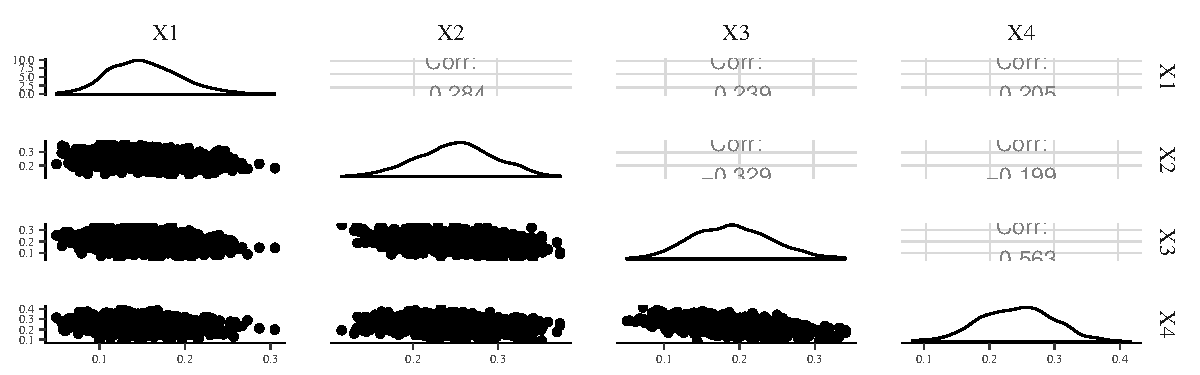
\includegraphics[width=\textwidth-3cm]{figure/ch03_figcovuncertainty-1} 

}


\begin{kframe}\begin{alltt}
\hlkwd{cov}\hlstd{(df[,}\hlnum{2}\hlopt{:}\hlnum{5}\hlstd{])}
\end{alltt}
\begin{verbatim}
##         x1      x2     x3     x4
## x1  0.8905 -0.0969 0.0377 0.1193
## x2 -0.0969  1.4187 0.0778 0.2580
## x3  0.0377  0.0778 1.0442 0.0341
## x4  0.1193  0.2580 0.0341 1.1203
\end{verbatim}
\end{kframe}
\end{knitrout}

\begin{knitrout}
\definecolor{shadecolor}{rgb}{0.98, 0.98, 0.98}\color{fgcolor}\begin{kframe}
\begin{alltt}
\hlcom{#Comparison of sample covariance and shrink covariance matrix}

\hlkwd{cov}\hlstd{(df[,}\hlnum{2}\hlopt{:}\hlnum{5}\hlstd{])}
\end{alltt}
\begin{verbatim}
##         x1      x2     x3     x4
## x1  0.8905 -0.0969 0.0377 0.1193
## x2 -0.0969  1.4187 0.0778 0.2580
## x3  0.0377  0.0778 1.0442 0.0341
## x4  0.1193  0.2580 0.0341 1.1203
\end{verbatim}
\begin{alltt}
\hlkwd{cov.shrink}\hlstd{(df[,}\hlnum{2}\hlopt{:}\hlnum{5}\hlstd{])}
\end{alltt}
\begin{verbatim}
## Estimating optimal shrinkage intensity lambda.var (variance vector): 1 
## 
## Estimating optimal shrinkage intensity lambda (correlation matrix): 1
##      x1   x2   x3   x4
## x1 1.08 0.00 0.00 0.00
## x2 0.00 1.08 0.00 0.00
## x3 0.00 0.00 1.08 0.00
## x4 0.00 0.00 0.00 1.08
## attr(,"lambda")
## [1] 1
## attr(,"lambda.estimated")
## [1] TRUE
## attr(,"class")
## [1] "shrinkage"
## attr(,"lambda.var")
## [1] 1
## attr(,"lambda.var.estimated")
## [1] TRUE
\end{verbatim}
\end{kframe}
\end{knitrout}

\section{Real World Data}


The following example data are taken from the book Bayesian Regression Modeling with INLA. The data were about air pollution in 41 cities in the United States originally published in Everitt (2006). The data consits of the SO2 level as the dependent variable and six explanatory variables 
Two of the explanatory variables are are related to human ecology (pop, manuf) and four others are related to climate (negtemp, wind, precip, days).


\begin{table}
\caption{Variable description of air pollution data}
\begin{tabularx}{\textwidth}{|l|X|l|}
  \hline			
  Variable Name & Description & Codes/Values \\   \hline  
  SO2 & sulfur dioxide content of air & microgrames per cubic meter \\
  negtemp & negative value of average & fahrenheit\\
  manuf & number of manufacturing enterprises employing 20 or more workers & integers \\
  pop & population size in thousands (1970 census) & numbers \\
  wind & average wind speed & miles per hour \\
  precip & average annual percipitation & inches \\
  days & average munber of days with precipitation per year & integers \\
  \hline  
\end{tabularx}
\label{table:airpollutiondata}
\end{table}



{\centering 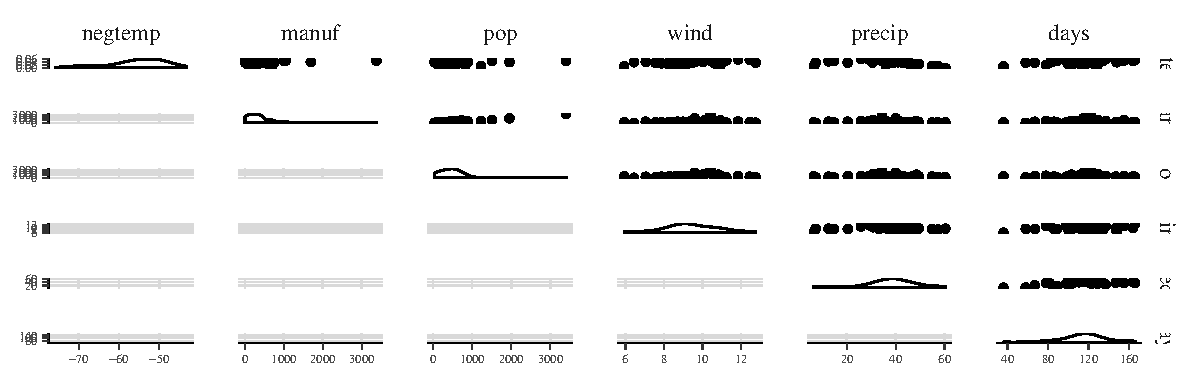
\includegraphics[width=\textwidth-3cm]{figure/ch03_figunnamed-chunk-4-1} 

}




A simple linear regression model including the dependent variable SO2 and the six explanatory variables is fitted with the lm command in R. The $R^2$ of the full model is 0.670. 

\begin{knitrout}
\definecolor{shadecolor}{rgb}{0.98, 0.98, 0.98}\color{fgcolor}\begin{kframe}
\begin{alltt}
\hlstd{usair.lm} \hlkwb{<-} \hlkwd{lm}\hlstd{(SO2}\hlopt{~}\hlstd{.,} \hlkwc{data} \hlstd{= usair)}


\hlcom{#Code assuming stochastic predictors}
\hlstd{run}\hlkwb{<-}\hlkwd{boot.relimp}\hlstd{(usair.lm,} \hlkwc{fixed}\hlstd{=}\hlnum{TRUE}\hlstd{)}

\hlkwd{booteval.relimp}\hlstd{(run,} \hlkwc{bty} \hlstd{=} \hlstr{"perc"}\hlstd{,} \hlkwc{level} \hlstd{=} \hlnum{0.95}\hlstd{,}
                \hlkwc{sort} \hlstd{=} \hlnum{FALSE}\hlstd{,} \hlkwc{norank} \hlstd{=} \hlnum{TRUE}\hlstd{,} \hlkwc{nodiff} \hlstd{=} \hlnum{TRUE}\hlstd{,}
                \hlkwc{typesel} \hlstd{=} \hlkwd{c}\hlstd{(}\hlstr{"lmg"}\hlstd{))}
\end{alltt}
\begin{verbatim}
## Response variable: SO2 
## Total response variance: 551 
## Analysis based on 41 observations 
## 
## 6 Regressors: 
## negtemp manuf pop wind precip days 
## Proportion of variance explained by model: 67%
## Metrics are not normalized (rela=FALSE). 
## 
## Relative importance metrics: 
## 
##            lmg
## negtemp 0.1111
## manuf   0.2965
## pop     0.1661
## wind    0.0167
## precip  0.0187
## days    0.0604
## 
## Average coefficients for different model sizes: 
## 
##             1X     2Xs      3Xs     4Xs     5Xs     6Xs
## negtemp 1.4081  1.3344  1.28118  1.2577  1.2826  1.2679
## manuf   0.0269  0.0373  0.04643  0.0539  0.0598  0.0649
## pop     0.0200  0.0044 -0.00925 -0.0207 -0.0304 -0.0393
## wind    1.5557 -0.0248 -1.38483 -2.3795 -2.9803 -3.1814
## precip  0.1083  0.1147  0.16427  0.2601  0.4057  0.5124
## days    0.3273  0.2979  0.24111  0.1557  0.0425 -0.0521
## 
##  
##  Confidence interval information ( 1000 bootstrap replicates, bty= perc ): 
## Relative Contributions with confidence intervals: 
##  
##                        Lower  Upper
##             percentage 0.95   0.95  
## negtemp.lmg 0.1111     0.0399 0.2206
## manuf.lmg   0.2965     0.2079 0.4126
## pop.lmg     0.1661     0.1134 0.2443
## wind.lmg    0.0167     0.0086 0.0718
## precip.lmg  0.0187     0.0075 0.0676
## days.lmg    0.0604     0.0187 0.1359
## 
## CAUTION: Bootstrap confidence intervals can be somewhat liberal. 
## NOTE: X-matrix has been considered as fixed for bootstrapping.
\end{verbatim}
\begin{alltt}
\hlstd{bayes.usair} \hlkwb{<-} \hlkwd{stan_glm}\hlstd{(SO2} \hlopt{~} \hlstd{. ,}
                  \hlkwc{data} \hlstd{= usair,}
                  \hlkwc{chains} \hlstd{=} \hlnum{4}\hlstd{,} \hlkwc{cores} \hlstd{=} \hlnum{4}\hlstd{)}

\hlcom{#posterior sample}
\hlstd{post.sample} \hlkwb{<-} \hlkwd{as.matrix}\hlstd{(bayes.usair)}

\hlcom{#example of the first 10 posterior samples}
\hlstd{post.sample[}\hlnum{1}\hlopt{:}\hlnum{10}\hlstd{,]}
\end{alltt}
\begin{verbatim}
##           parameters
## iterations (Intercept) negtemp  manuf     pop  wind precip    days sigma
##       [1,]       154.7    1.47 0.0610 -0.0321 -5.29  0.310 -0.1161  12.9
##       [2,]       138.4    1.47 0.0510 -0.0286 -4.69  0.199  0.0271  13.0
##       [3,]       159.8    1.71 0.0386 -0.0104 -6.89  0.601 -0.0297  12.8
##       [4,]       135.3    2.07 0.0392 -0.0178 -1.05  1.245 -0.2573  20.0
##       [5,]       220.5    2.51 0.0621 -0.0385 -7.49  1.210 -0.2822  12.2
##       [6,]       151.5    1.64 0.0625 -0.0395 -4.38  0.701 -0.1878  13.2
##       [7,]        95.2    1.13 0.0646 -0.0427 -2.64  0.393  0.0238  13.2
##       [8,]       178.4    2.09 0.0588 -0.0401 -4.25  0.752 -0.1822  16.1
##       [9,]       182.5    1.94 0.0528 -0.0233 -7.38  0.661 -0.0920  15.7
##      [10,]       129.2    1.48 0.0596 -0.0364 -4.12  0.466 -0.0031  11.6
\end{verbatim}
\begin{alltt}
\hlcom{#no need for the intercept, last parameter is sigma}
\hlstd{post.sample} \hlkwb{<-} \hlstd{post.sample[,}\hlopt{-}\hlnum{1}\hlstd{]}

\hlcom{#data frame with all submodels}
\hlstd{df.rtwos} \hlkwb{<-}\hlkwd{rtwos}\hlstd{(usair[,}\hlnum{2}\hlopt{:}\hlnum{7}\hlstd{], post.sample)}

\hlstd{df.rtwos[,}\hlnum{1}\hlopt{:}\hlnum{3}\hlstd{]}
\end{alltt}
\begin{verbatim}
##                      X1       X2      X3
## none           0.00e+00 0.000000 0.00000
## x1             1.97e-01 0.284523 0.16279
## x2             4.66e-01 0.347261 0.43399
## x3             3.00e-01 0.198395 0.30876
## x4             4.83e-05 0.000313 0.00610
## x5             1.10e-02 0.006372 0.00394
## x6             5.92e-02 0.138557 0.14439
## x1 x2          5.68e-01 0.531508 0.51433
## x1 x3          4.68e-01 0.454922 0.44519
## x1 x4          2.27e-01 0.317017 0.21754
## x1 x5          2.02e-01 0.303245 0.21897
## x1 x6          2.01e-01 0.309526 0.21506
## x2 x3          5.91e-01 0.505155 0.49602
## x2 x4          4.96e-01 0.363178 0.49247
## x2 x5          4.73e-01 0.350951 0.44108
## x2 x6          4.90e-01 0.435553 0.52144
## x3 x4          3.15e-01 0.204610 0.34911
## x3 x5          3.08e-01 0.203048 0.31474
## x3 x6          3.48e-01 0.323570 0.43615
## x4 x5          1.11e-02 0.006649 0.00992
## x4 x6          6.14e-02 0.140494 0.16467
## x5 x6          1.27e-01 0.231347 0.16535
## x1 x2 x3       6.28e-01 0.590520 0.53559
## x1 x2 x4       6.54e-01 0.608672 0.63732
## x1 x2 x5       5.70e-01 0.544606 0.55860
## x1 x2 x6       5.69e-01 0.548474 0.55253
## x1 x3 x4       5.50e-01 0.527898 0.56752
## x1 x3 x5       4.74e-01 0.473879 0.50190
## x1 x3 x6       4.71e-01 0.477789 0.49348
## x1 x4 x5       2.37e-01 0.343893 0.29198
## x1 x4 x6       2.31e-01 0.342953 0.27157
## x1 x5 x6       2.02e-01 0.309859 0.22335
## x2 x3 x4       6.28e-01 0.526656 0.56098
## x2 x3 x5       5.97e-01 0.508097 0.50382
## x2 x3 x6       5.94e-01 0.541822 0.55090
## x2 x4 x5       5.03e-01 0.366953 0.49934
## x2 x4 x6       5.29e-01 0.464027 0.60285
## x2 x5 x6       5.25e-01 0.495216 0.52714
## x3 x4 x5       3.24e-01 0.209346 0.35485
## x3 x4 x6       3.75e-01 0.342287 0.50422
## x3 x5 x6       4.02e-01 0.402940 0.44953
## x4 x5 x6       1.33e-01 0.237439 0.19074
## x1 x2 x3 x4    7.01e-01 0.656304 0.65030
## x1 x2 x3 x5    6.28e-01 0.596064 0.57111
## x1 x2 x3 x6    6.28e-01 0.599999 0.56687
## x1 x2 x4 x5    6.61e-01 0.632223 0.70506
## x1 x2 x4 x6    6.54e-01 0.626054 0.67631
## x1 x2 x5 x6    5.71e-01 0.548797 0.56076
## x1 x3 x4 x5    5.63e-01 0.559821 0.65269
## x1 x3 x4 x6    5.52e-01 0.551841 0.61783
## x1 x3 x5 x6    4.74e-01 0.478612 0.50440
## x1 x4 x5 x6    2.38e-01 0.346356 0.29252
## x2 x3 x4 x5    6.34e-01 0.529672 0.56857
## x2 x3 x4 x6    6.35e-01 0.571661 0.63352
## x2 x3 x5 x6    6.10e-01 0.575817 0.55275
## x2 x4 x5 x6    5.71e-01 0.531670 0.61303
## x3 x4 x5 x6    4.37e-01 0.430562 0.52463
## x1 x2 x3 x4 x5 7.03e-01 0.669594 0.70958
## x1 x2 x3 x4 x6 7.01e-01 0.666749 0.68389
## x1 x2 x3 x5 x6 6.28e-01 0.600015 0.57319
## x1 x2 x4 x5 x6 6.66e-01 0.632442 0.70541
## x1 x3 x4 x5 x6 5.68e-01 0.560186 0.65296
## x2 x3 x4 x5 x6 6.56e-01 0.611735 0.63818
## all            7.08e-01 0.669885 0.70990
\end{verbatim}
\begin{alltt}
\hlcom{# prepare data frame for LMG values}

\hlstd{LMG.Vals.I}\hlkwb{<-}\hlkwd{matrix}\hlstd{(}\hlnum{0}\hlstd{,} \hlnum{6}\hlstd{,} \hlkwd{dim}\hlstd{(df.rtwos)[}\hlnum{2}\hlstd{])}

\hlkwa{for}\hlstd{(i} \hlkwa{in} \hlnum{1}\hlopt{:}\hlkwd{dim}\hlstd{(df.rtwos)[}\hlnum{2}\hlstd{])\{}

  \hlstd{gofn}\hlkwb{<-}\hlstd{df.rtwos[,i]}

  \hlstd{obj.Gelman}\hlkwb{<-}\hlkwd{partition}\hlstd{(gofn,} \hlkwc{pcan} \hlstd{=} \hlnum{6}\hlstd{,} \hlkwc{var.names} \hlstd{=} \hlkwd{names}\hlstd{(usair[,}\hlnum{2}\hlopt{:}\hlnum{7}\hlstd{]))}

  \hlstd{LMG.Vals.I[,i]}\hlkwb{=}\hlstd{obj.Gelman}\hlopt{$}\hlstd{IJ[,}\hlnum{1}\hlstd{]}
\hlstd{\}}

\hlcom{# posterior LMG distribution of each variable}
\hlkwd{quantile}\hlstd{(LMG.Vals.I[}\hlnum{1}\hlstd{,],} \hlkwd{c}\hlstd{(}\hlnum{0.025}\hlstd{,} \hlnum{0.5}\hlstd{,} \hlnum{0.975}\hlstd{))}
\end{alltt}
\begin{verbatim}
##   2.5%    50%  97.5% 
## 0.0341 0.1038 0.2061
\end{verbatim}
\begin{alltt}
\hlkwd{quantile}\hlstd{(LMG.Vals.I[}\hlnum{2}\hlstd{,],} \hlkwd{c}\hlstd{(}\hlnum{0.025}\hlstd{,} \hlnum{0.5}\hlstd{,} \hlnum{0.975}\hlstd{))}
\end{alltt}
\begin{verbatim}
##  2.5%   50% 97.5% 
## 0.151 0.265 0.361
\end{verbatim}
\begin{alltt}
\hlkwd{quantile}\hlstd{(LMG.Vals.I[}\hlnum{3}\hlstd{,],} \hlkwd{c}\hlstd{(}\hlnum{0.025}\hlstd{,} \hlnum{0.5}\hlstd{,} \hlnum{0.975}\hlstd{))}
\end{alltt}
\begin{verbatim}
##   2.5%    50%  97.5% 
## 0.0871 0.1527 0.2121
\end{verbatim}
\begin{alltt}
\hlkwd{quantile}\hlstd{(LMG.Vals.I[}\hlnum{4}\hlstd{,],} \hlkwd{c}\hlstd{(}\hlnum{0.025}\hlstd{,} \hlnum{0.5}\hlstd{,} \hlnum{0.975}\hlstd{))}
\end{alltt}
\begin{verbatim}
##    2.5%     50%   97.5% 
## 0.00759 0.01680 0.07210
\end{verbatim}
\begin{alltt}
\hlkwd{quantile}\hlstd{(LMG.Vals.I[}\hlnum{5}\hlstd{,],} \hlkwd{c}\hlstd{(}\hlnum{0.025}\hlstd{,} \hlnum{0.5}\hlstd{,} \hlnum{0.975}\hlstd{))}
\end{alltt}
\begin{verbatim}
##    2.5%     50%   97.5% 
## 0.00692 0.02045 0.07085
\end{verbatim}
\begin{alltt}
\hlkwd{quantile}\hlstd{(LMG.Vals.I[}\hlnum{6}\hlstd{,],} \hlkwd{c}\hlstd{(}\hlnum{0.025}\hlstd{,} \hlnum{0.5}\hlstd{,} \hlnum{0.975}\hlstd{))}
\end{alltt}
\begin{verbatim}
##   2.5%    50%  97.5% 
## 0.0180 0.0577 0.1318
\end{verbatim}
\begin{alltt}
\hlcom{#Visualization}
\hlstd{dat} \hlkwb{<-} \hlkwd{data.frame}\hlstd{(}\hlkwd{t}\hlstd{(LMG.Vals.I))}

\hlstd{pairs.chart} \hlkwb{<-} \hlkwd{ggpairs}\hlstd{(dat,} \hlkwc{lower} \hlstd{=} \hlkwd{list}\hlstd{(}\hlkwd{list}\hlstd{(}\hlkwc{combo} \hlstd{=} \hlstr{"facetdensity"}\hlstd{)),} \hlkwc{upper} \hlstd{=} \hlkwd{list}\hlstd{(}\hlkwd{list}\hlstd{(}\hlkwc{continuous} \hlstd{=} \hlstr{"cor"}\hlstd{)))} \hlopt{+} \hlstd{ggplot2}\hlopt{::}\hlkwd{theme}\hlstd{(}\hlkwc{axis.text} \hlstd{=} \hlkwd{element_text}\hlstd{(}\hlkwc{size} \hlstd{=} \hlnum{6}\hlstd{))}
\hlstd{pairs.chart}
\end{alltt}
\end{kframe}

{\centering 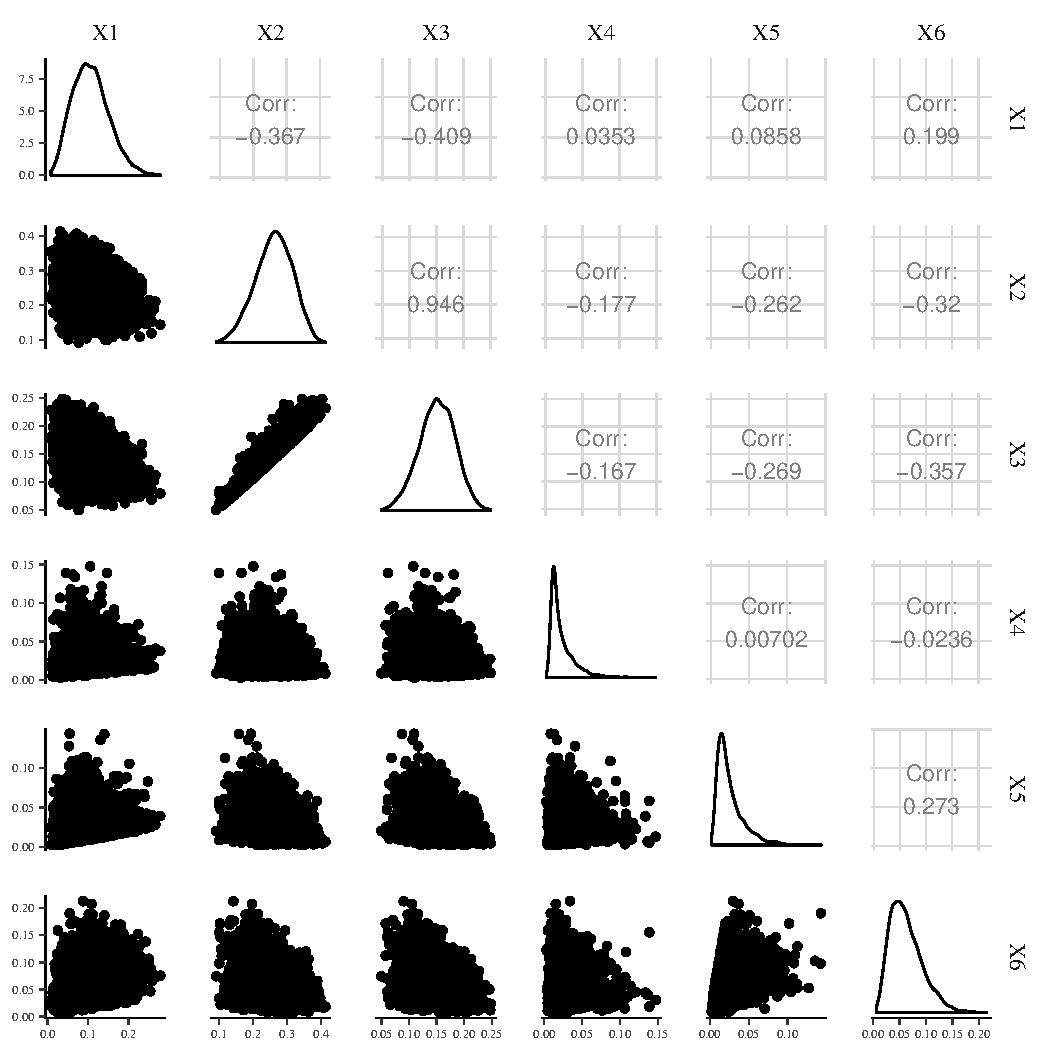
\includegraphics[width=\textwidth-3cm]{figure/ch03_figreal_data_LMG-1} 

}


\begin{kframe}\begin{alltt}
\hlcom{#use prior knowledge}
\hlstd{my_prior} \hlkwb{<-} \hlkwd{normal}\hlstd{(}\hlkwc{location} \hlstd{=} \hlkwd{c}\hlstd{(}\hlnum{1}\hlstd{,} \hlnum{0.05}\hlstd{,}\hlopt{-}\hlnum{0.03}\hlstd{,}\hlopt{-}\hlnum{3}\hlstd{,} \hlnum{0}\hlstd{,} \hlnum{0}\hlstd{),} \hlkwc{scale} \hlstd{=} \hlkwd{c}\hlstd{(}\hlnum{0.1}\hlstd{,} \hlnum{0.01}\hlstd{,}\hlnum{0.01}\hlstd{,}\hlnum{0.1}\hlstd{,} \hlnum{0.1}\hlstd{,} \hlnum{0.1}\hlstd{),} \hlkwc{autoscale} \hlstd{=} \hlnum{FALSE}\hlstd{)}


\hlstd{bayes.usair} \hlkwb{<-} \hlkwd{stan_glm}\hlstd{(SO2} \hlopt{~} \hlstd{. ,}
                  \hlkwc{data} \hlstd{= usair,} \hlkwc{prior} \hlstd{= my_prior,}
                  \hlkwc{chains} \hlstd{=} \hlnum{4}\hlstd{,} \hlkwc{cores} \hlstd{=} \hlnum{4}\hlstd{)}

\hlcom{#posterior sample}
\hlstd{post.sample} \hlkwb{<-} \hlkwd{as.matrix}\hlstd{(bayes.usair)}

\hlcom{#example of the first 10 posterior samples}
\hlstd{post.sample[}\hlnum{1}\hlopt{:}\hlnum{10}\hlstd{,]}
\end{alltt}
\begin{verbatim}
##           parameters
## iterations (Intercept) negtemp  manuf     pop  wind  precip    days sigma
##       [1,]       106.3   1.213 0.0487 -0.0305 -3.00  0.2553  0.0546  14.8
##       [2,]        97.0   0.804 0.0560 -0.0334 -2.95 -0.1191  0.0282  15.3
##       [3,]        89.5   0.855 0.0583 -0.0304 -2.96 -0.0258  0.0663  13.8
##       [4,]        98.3   0.850 0.0586 -0.0372 -3.05 -0.0598  0.0412  12.7
##       [5,]        94.3   0.865 0.0648 -0.0318 -3.04 -0.0657  0.0409  13.5
##       [6,]        78.6   0.937 0.0528 -0.0255 -2.97  0.2033  0.1282  13.3
##       [7,]       111.7   0.999 0.0557 -0.0268 -3.04 -0.0527 -0.0426  16.1
##       [8,]        85.6   0.960 0.0510 -0.0295 -2.95  0.1638  0.1298  12.6
##       [9,]        92.9   1.003 0.0645 -0.0373 -3.00  0.0568  0.1140  15.3
##      [10,]       101.4   1.118 0.0520 -0.0284 -3.03  0.1328  0.0661  11.8
\end{verbatim}
\begin{alltt}
\hlcom{#no need for the intercept, last parameter is sigma}
\hlstd{post.sample} \hlkwb{<-} \hlstd{post.sample[,}\hlopt{-}\hlnum{1}\hlstd{]}

\hlcom{#data frame with all submodels}
\hlstd{df.rtwos} \hlkwb{<-}\hlkwd{rtwos}\hlstd{(usair[,}\hlnum{2}\hlopt{:}\hlnum{7}\hlstd{], post.sample)}


\hlcom{# prepare data frame for LMG values}

\hlstd{LMG.Vals.I}\hlkwb{<-}\hlkwd{matrix}\hlstd{(}\hlnum{0}\hlstd{,} \hlnum{6}\hlstd{,} \hlkwd{dim}\hlstd{(df.rtwos)[}\hlnum{2}\hlstd{])}

\hlkwa{for}\hlstd{(i} \hlkwa{in} \hlnum{1}\hlopt{:}\hlkwd{dim}\hlstd{(df.rtwos)[}\hlnum{2}\hlstd{])\{}

  \hlstd{gofn}\hlkwb{<-}\hlstd{df.rtwos[,i]}

  \hlstd{obj.Gelman}\hlkwb{<-}\hlkwd{partition}\hlstd{(gofn,} \hlkwc{pcan} \hlstd{=} \hlnum{6}\hlstd{,} \hlkwc{var.names} \hlstd{=} \hlkwd{names}\hlstd{(usair[,}\hlnum{2}\hlopt{:}\hlnum{7}\hlstd{]))}

  \hlstd{LMG.Vals.I[,i]}\hlkwb{=}\hlstd{obj.Gelman}\hlopt{$}\hlstd{IJ[,}\hlnum{1}\hlstd{]}
\hlstd{\}}

\hlcom{# posterior LMG distribution of each variable}
\hlkwd{quantile}\hlstd{(LMG.Vals.I[}\hlnum{1}\hlstd{,],} \hlkwd{c}\hlstd{(}\hlnum{0.025}\hlstd{,} \hlnum{0.5}\hlstd{,} \hlnum{0.975}\hlstd{))}
\end{alltt}
\begin{verbatim}
##   2.5%    50%  97.5% 
## 0.0734 0.1138 0.1594
\end{verbatim}
\begin{alltt}
\hlkwd{quantile}\hlstd{(LMG.Vals.I[}\hlnum{2}\hlstd{,],} \hlkwd{c}\hlstd{(}\hlnum{0.025}\hlstd{,} \hlnum{0.5}\hlstd{,} \hlnum{0.975}\hlstd{))}
\end{alltt}
\begin{verbatim}
##  2.5%   50% 97.5% 
## 0.171 0.259 0.334
\end{verbatim}
\begin{alltt}
\hlkwd{quantile}\hlstd{(LMG.Vals.I[}\hlnum{3}\hlstd{,],} \hlkwd{c}\hlstd{(}\hlnum{0.025}\hlstd{,} \hlnum{0.5}\hlstd{,} \hlnum{0.975}\hlstd{))}
\end{alltt}
\begin{verbatim}
##   2.5%    50%  97.5% 
## 0.0947 0.1510 0.2083
\end{verbatim}
\begin{alltt}
\hlkwd{quantile}\hlstd{(LMG.Vals.I[}\hlnum{4}\hlstd{,],} \hlkwd{c}\hlstd{(}\hlnum{0.025}\hlstd{,} \hlnum{0.5}\hlstd{,} \hlnum{0.975}\hlstd{))}
\end{alltt}
\begin{verbatim}
##   2.5%    50%  97.5% 
## 0.0128 0.0163 0.0214
\end{verbatim}
\begin{alltt}
\hlkwd{quantile}\hlstd{(LMG.Vals.I[}\hlnum{5}\hlstd{,],} \hlkwd{c}\hlstd{(}\hlnum{0.025}\hlstd{,} \hlnum{0.5}\hlstd{,} \hlnum{0.975}\hlstd{))}
\end{alltt}
\begin{verbatim}
##    2.5%     50%   97.5% 
## 0.00782 0.01310 0.02503
\end{verbatim}
\begin{alltt}
\hlkwd{quantile}\hlstd{(LMG.Vals.I[}\hlnum{6}\hlstd{,],} \hlkwd{c}\hlstd{(}\hlnum{0.025}\hlstd{,} \hlnum{0.5}\hlstd{,} \hlnum{0.975}\hlstd{))}
\end{alltt}
\begin{verbatim}
##   2.5%    50%  97.5% 
## 0.0166 0.0515 0.1076
\end{verbatim}
\begin{alltt}
\hlcom{#Visualization}
\hlstd{dat} \hlkwb{<-} \hlkwd{data.frame}\hlstd{(}\hlkwd{t}\hlstd{(LMG.Vals.I))}

\hlstd{pairs.chart} \hlkwb{<-} \hlkwd{ggpairs}\hlstd{(dat,} \hlkwc{lower} \hlstd{=} \hlkwd{list}\hlstd{(}\hlkwd{list}\hlstd{(}\hlkwc{combo} \hlstd{=} \hlstr{"facetdensity"}\hlstd{)),} \hlkwc{upper} \hlstd{=} \hlkwd{list}\hlstd{(}\hlkwd{list}\hlstd{(}\hlkwc{continuous} \hlstd{=} \hlstr{"cor"}\hlstd{)))} \hlopt{+} \hlstd{ggplot2}\hlopt{::}\hlkwd{theme}\hlstd{(}\hlkwc{axis.text} \hlstd{=} \hlkwd{element_text}\hlstd{(}\hlkwc{size} \hlstd{=} \hlnum{6}\hlstd{))}
\hlstd{pairs.chart}
\end{alltt}
\end{kframe}

{\centering 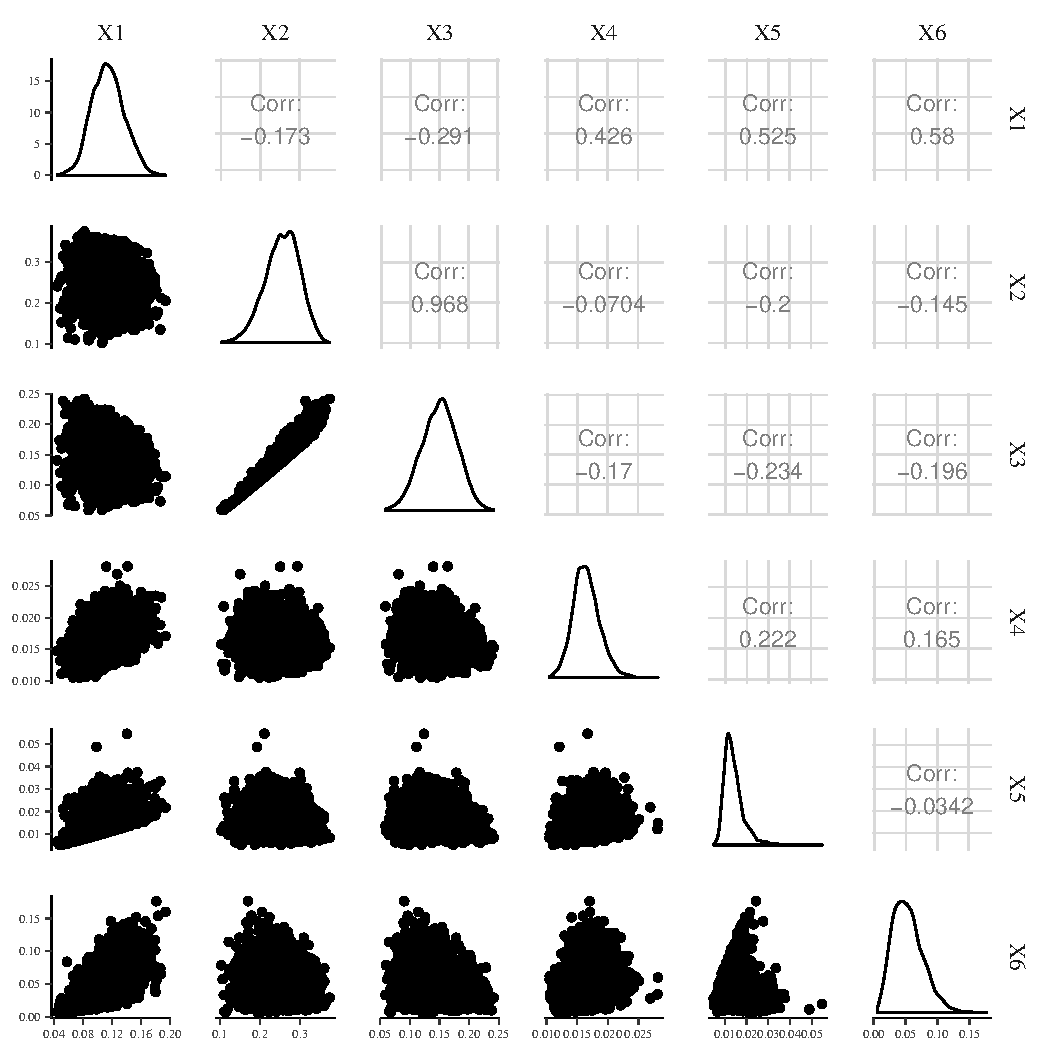
\includegraphics[width=\textwidth-3cm]{figure/ch03_figreal_data_LMG-2} 

}



\end{knitrout}










% LaTeX file for Chapter 04





\chapter{Discussion and Outlook - Some extenstions}

In the following chapter some extenstions of the LMG formula in the Bayesian framework beyond the simple linear regression model are shown. The focus is on repeated measurements models. These models extend the simple linear regression be allowing intra subject correlation between repeated measures. 

The dependence within subjects can be modeled by including random effects (mixed model) or by assuming correlated errors within a subject (marginal model). Using a random intercept model or a compound symmetry matrix for the error will result in the same model for the fixed predictors. A mixed model can be extended by including a random slope per subject, allowing for less restrictive longitudinal shapes. The marginal approach can get more freedom by different specified covariance matrices of the error terms. An unstructured covariance matrix, where no restriction are imposed, allows for the most freedom. However, depending on the number of repeated measuresments and the sample size the covariance matrix can get too large to make reasonable inference about it. 


The extenstion of the LMG formula in the Bayesian framework presented in chapter is restricted to models where the conditional variance formula can easily be applied to get the explained variance of the submodel from the regression parameters of the full model. The focus is on the fixed predictors and not on the random effects. Using the conditional variance formula to get the explained variance of the fixed predictors of the submodels should be applicable in the marginal models, where only the fixed effects are modelled anyway. In the mixed model framework the conditional variance formula is applicable to models including only random intercepts and the focus lies in the explained variance of the fixed predictors. For random-slope models there are atleast some difficulties involved, if it is possible at all the get the expalined variance of the submodel. This chapter shows a  random intercept model and a repeated measurement model with an unstructured covariance matrix.  

The first example concerns a simple random intercept model with time varying predictors.  

\section{random intercept model}

Different $\Rtwo$ metrics exist for linear mixed models. The variance of a random intercept model with regression parameter $\bbeta$ can be written as

      \begin{align} 
        \var(y) = \sigma_{f}^2  + \sigma_{\alpha}^2 + \sigma_{\epsilon}^2, 
        \end{align}

where $\sigma_{f}^2 = \var(\X \bbeta) = \bbeta^\top \bSigma_{\X \X}  \bbeta$ , $\sigma_{\alpha}^2 $ is the random intercept and $\sigma_{\epsilon}^2$ is the error term. 

An $\Rtwo$ that is guaranteed to be positive can be defined as

   \begin{align} 
\Rtwo_{\text{LMM}} = \frac{\sigma_{f}^2}{\sigma_{f}^2 + \sigma_{\alpha}^2 + \sigma_{\epsilon}^2},
\end{align}

Referenz Naka, Snyder.... It is theoretical possible that the $\Rtwo_{\text{LMM}}$ decreases when adding predictors. This may be problematic for the LMG metric, because of violation of the non-negative property. This should rarely be the case with real data. The $\Rtwo$ can not decrease when adding predictor by using the conditional variance formula on the full model to calculate the $\Rtwo$ of the submodels. In the Bayesian framework we would the sample from the posterior distributions of the parameters. 

The total variance of the full can be calculated as in equation 6 or by using the samples of the random intercept for each subject directly. The same total variance is then used for one sample of the posterior. (In a repeated measure study we often have within and between subject predictors. If we use the total variance of the full model the random intercept is fitted including all predictors. If a between subject predictor is excluded (e.g. Sex) and we would fit a new random intercept model, the random intercept parameter will in addition explain the variance that was explained by the excluded predictor. In other words it means that the model with the exluded between subject predictor will explain almost as much as the model where the predictor is included when each time a new model and therefore a new random intercept term is fitted in each model. 

When using the conditional variance formula for the $\Rtwo$ of the submodels, it only takes into account the explained variance of the fixed predictors. )


In repeated measurement studies the focus is often in within subject changes. The between subject variance estimated with the random intercept term may not be so important. The more important question may be how much the fixed predictors explain compared to the within subject error, which is

   \begin{align} 
\Rtwo_{\text{repeated}} = \frac{\sigma_{f}^2}{\sigma_{f}^2  + \sigma_{\epsilon}^2},
\end{align}

The square root of this term is known under the name correlation within subjects by ref(bland Altman 1995). Although in the paper the subject term is fitted as a factor. If we are interested in the within subject effects we can use the model including only the between subject predictor as the null model.

The following example shows a simple random intercept model with time-varying predictors. The main question is which within subject predictors are the most important ones. The between subject variance is of lower importance. 

The data are simulated from the following regression setting with $m = 4$ timepoints,

\begin{align} 
&Y_{i,j} \sim \mathcal{N}(\beta_{0}+x_{1_{i,j}} \beta_{1}+x_{2_{i,j}} \beta_{2}+x_{3_{i,j}} \beta_{3}+x_{4_{i,j}} \beta_{4} + \alpha_{i}, \, \sigma^2), \qquad i = 1, \dots, n \qquad j = 1, \dots, m
\end{align} 

where $\beta_{1} = 1$, $\beta_{2} = 1$,  $\beta_{3} = 2$ , $\beta_{4}=2$, $\sigma^2 = 1$, $\alpha_{i} \sim \mathcal{N}(0, \sigma_{\alpha}^2)$, $\X \sim \mathcal{N}(\0, \bSigma)$.

The following R code is used to simulate the data:



\begin{knitrout}
\definecolor{shadecolor}{rgb}{0.98, 0.98, 0.98}\color{fgcolor}\begin{kframe}
\begin{alltt}
\hlstd{sub}\hlkwb{<-} \hlnum{1}\hlopt{:}\hlnum{20}
\hlstd{subi} \hlkwb{<-} \hlkwd{rnorm}\hlstd{(}\hlnum{20}\hlstd{,} \hlnum{0}\hlstd{,} \hlnum{4}\hlstd{)}
\hlstd{subi}\hlkwb{<-}\hlkwd{rep}\hlstd{(subi,} \hlnum{4}\hlstd{)}
\hlstd{t} \hlkwb{<-} \hlkwd{c}\hlstd{(}\hlnum{0}\hlstd{,} \hlnum{1}\hlstd{,} \hlnum{2}\hlstd{,}\hlnum{3}\hlstd{)}
\hlstd{t} \hlkwb{<-} \hlkwd{c}\hlstd{(}\hlkwd{rep}\hlstd{(}\hlnum{0}\hlstd{,} \hlnum{20}\hlstd{),} \hlkwd{rep}\hlstd{(}\hlnum{1}\hlstd{,}\hlnum{20}\hlstd{),} \hlkwd{rep}\hlstd{(}\hlnum{2}\hlstd{,} \hlnum{20}\hlstd{),} \hlkwd{rep}\hlstd{(}\hlnum{3}\hlstd{,}\hlnum{20}\hlstd{))}

\hlstd{mu} \hlkwb{<-} \hlkwd{rep}\hlstd{(}\hlnum{0}\hlstd{,}\hlnum{4}\hlstd{)}
\hlstd{sig} \hlkwb{<-} \hlkwd{matrix}\hlstd{(}\hlnum{0.4}\hlstd{,} \hlnum{4}\hlstd{,} \hlnum{4}\hlstd{)}
\hlkwd{diag}\hlstd{(sig)} \hlkwb{<-} \hlnum{1}
\hlstd{sig[}\hlnum{3}\hlstd{,}\hlnum{4}\hlstd{]} \hlkwb{<-} \hlnum{0.9}
\hlstd{sig[}\hlnum{4}\hlstd{,}\hlnum{3}\hlstd{]} \hlkwb{<-} \hlnum{0.9}
\hlstd{sig[}\hlnum{1}\hlstd{,}\hlnum{2}\hlstd{]} \hlkwb{<-} \hlnum{0.3}
\hlstd{sig[}\hlnum{2}\hlstd{,}\hlnum{1}\hlstd{]} \hlkwb{<-} \hlnum{0.3}


\hlstd{rawvars} \hlkwb{<-} \hlkwd{mvrnorm}\hlstd{(}\hlkwc{n}\hlstd{=}\hlnum{80}\hlstd{,} \hlkwc{mu}\hlstd{=mu,} \hlkwc{Sigma}\hlstd{=sig)}

\hlstd{x1} \hlkwb{<-} \hlstd{t}\hlopt{+}\hlstd{rawvars[,}\hlnum{1}\hlstd{]}
\hlstd{x2} \hlkwb{<-} \hlstd{t}\hlopt{+}\hlstd{rawvars[,}\hlnum{2}\hlstd{]}
\hlstd{x3} \hlkwb{<-} \hlstd{t}\hlopt{+}\hlstd{rawvars[,}\hlnum{3}\hlstd{]}
\hlstd{x4} \hlkwb{<-} \hlstd{t}\hlopt{+}\hlstd{rawvars[,}\hlnum{4}\hlstd{]}

\hlstd{b1} \hlkwb{<-} \hlstd{b2}  \hlkwb{<-}\hlnum{1}
\hlstd{b3} \hlkwb{<-} \hlstd{b4} \hlkwb{<-} \hlnum{2}

\hlstd{y}\hlkwb{<-} \hlstd{x1}\hlopt{*}\hlstd{b1} \hlopt{+}\hlstd{x2}\hlopt{*}\hlstd{b2} \hlopt{+}\hlstd{x3}\hlopt{*}\hlstd{b3}\hlopt{+}  \hlstd{x4}\hlopt{*}\hlstd{b4} \hlopt{+} \hlstd{subi}\hlopt{+} \hlkwd{rnorm}\hlstd{(}\hlnum{80}\hlstd{,} \hlnum{0}\hlstd{,} \hlnum{0.1}\hlstd{)}

\hlstd{df} \hlkwb{<-} \hlkwd{data.frame}\hlstd{(}\hlkwc{y}\hlstd{=y,} \hlkwc{x1} \hlstd{= x1,} \hlkwc{x2}\hlstd{=x2,} \hlkwc{x3} \hlstd{= x3,} \hlkwc{x4} \hlstd{= x4,} \hlkwc{sub} \hlstd{=} \hlkwd{rep}\hlstd{(sub,}\hlnum{4}\hlstd{))}

\hlstd{p} \hlkwb{<-} \hlkwd{ggplot}\hlstd{(}\hlkwc{data} \hlstd{= df,} \hlkwd{aes}\hlstd{(}\hlkwc{x} \hlstd{= t,} \hlkwc{y} \hlstd{= y,} \hlkwc{group} \hlstd{= sub))}
\hlstd{p} \hlopt{+} \hlkwd{geom_line}\hlstd{()}
\end{alltt}
\end{kframe}

{\centering 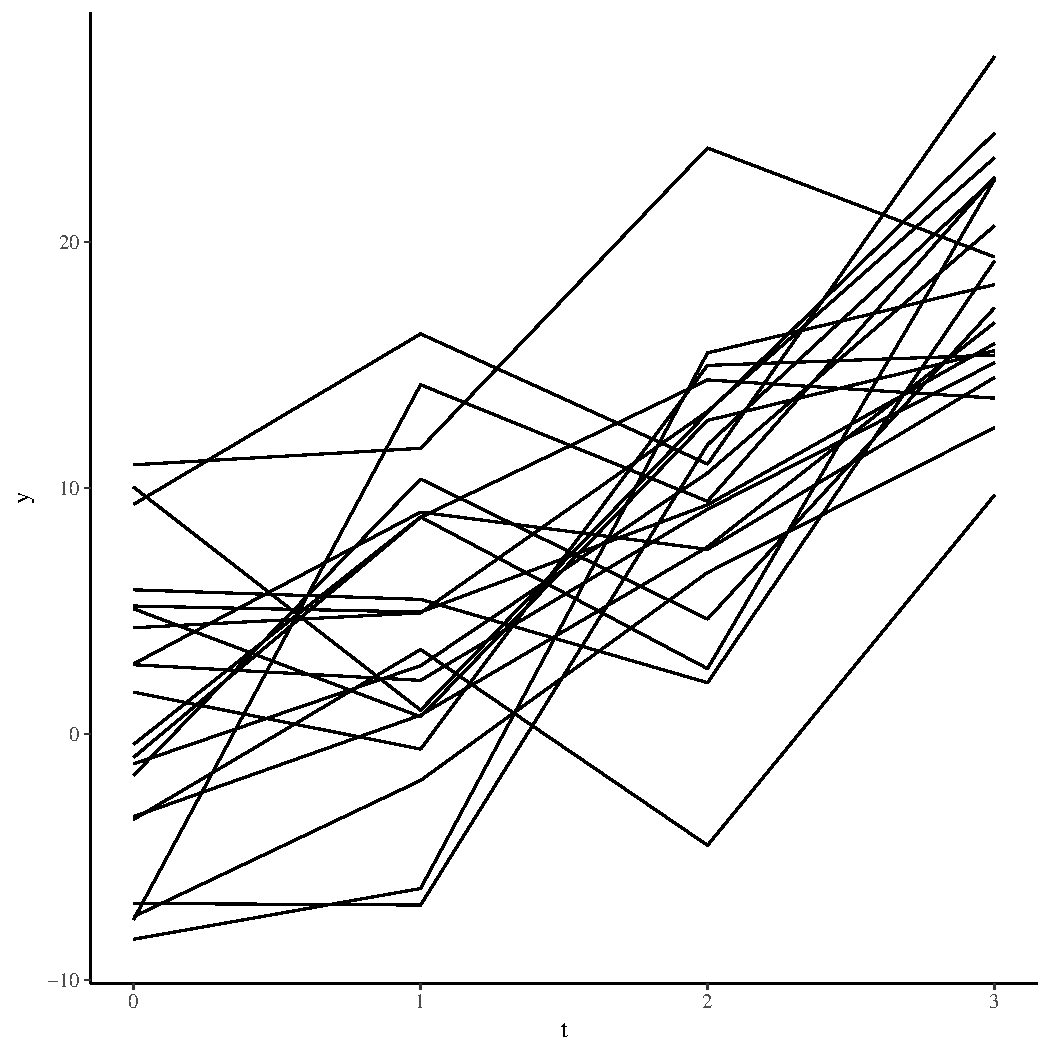
\includegraphics[width=\textwidth-3cm]{figure/ch04_figsimdata_repeated-1} 

}



\end{knitrout}


The $\Rtwo$ of the submodels were first calculated according to the formula in equation ...,. The random intercept effect is not of interest. We see that most of the within subject variance is explained by the predictors. The credible intervals are very narrow. For the information about the between subject varinace we can look at the random intercept variance directly. In the second part the random intercept is included in the total variance calculation and the calculation of the $\Rtwo$ values. We see that there is a large between subject variance in this dataset. The LMG values including the between subject variance are much lower. The credible intervals are also much wider, because the uncertainty about the between subject variance is also included. In my opinion we can get more useful infromation from separating the between and within variance components when it is easy possible. Note that we assumed non stochastic predictors otherwise the credible intervals would be larger. In general it seems more reasonable to assume stochastic time-varying predictors. The variance could then be estimated by non-parameteric bootstrap, resampling whole subjects (all repeated measurements of a subject).


\begin{knitrout}
\definecolor{shadecolor}{rgb}{0.98, 0.98, 0.98}\color{fgcolor}\begin{kframe}
\begin{alltt}
\hlstd{fit} \hlkwb{<-} \hlkwd{stan_glmer}\hlstd{(y} \hlopt{~} \hlstd{x1}\hlopt{+}\hlstd{x2}\hlopt{+}\hlstd{x3}\hlopt{+}\hlstd{x4} \hlopt{+} \hlstd{(}\hlnum{1}\hlopt{|}\hlstd{sub) ,}
                                                                        \hlkwc{data} \hlstd{= df,}
                                                                        \hlkwc{chains} \hlstd{=} \hlnum{4}\hlstd{,} \hlkwc{cores} \hlstd{=} \hlnum{4}\hlstd{)}

\hlstd{post.sample} \hlkwb{<-} \hlkwd{as.matrix}\hlstd{(fit)}
\hlstd{post.sample.r} \hlkwb{<-} \hlstd{post.sample[,}\hlkwd{c}\hlstd{(}\hlnum{2}\hlopt{:}\hlnum{5}\hlstd{,(}\hlkwd{ncol}\hlstd{(post.sample)}\hlopt{-}\hlnum{1}\hlstd{)}\hlopt{:}\hlkwd{ncol}\hlstd{(post.sample))]}

\hlstd{df.rtwos} \hlkwb{<-} \hlkwd{rtwos.ri.r}\hlstd{(df[,}\hlnum{2}\hlopt{:}\hlnum{5}\hlstd{], post.sample.r)}


\hlstd{LMG.Vals}\hlkwb{<-}\hlkwd{matrix}\hlstd{(}\hlnum{0}\hlstd{,} \hlnum{4}\hlstd{,} \hlkwd{dim}\hlstd{(df.rtwos)[}\hlnum{2}\hlstd{])}

\hlkwa{for}\hlstd{(i} \hlkwa{in} \hlnum{1}\hlopt{:}\hlkwd{dim}\hlstd{(df.rtwos)[}\hlnum{2}\hlstd{])\{}

        \hlstd{gofn}\hlkwb{<-}\hlstd{df.rtwos[,i]}

        \hlstd{obj.Gelman}\hlkwb{<-}\hlkwd{partition}\hlstd{(gofn,} \hlkwc{pcan} \hlstd{=} \hlnum{4}\hlstd{,} \hlkwc{var.names} \hlstd{=} \hlkwd{names}\hlstd{(df[,}\hlnum{2}\hlopt{:}\hlnum{5}\hlstd{]))}

        \hlstd{LMG.Vals[,i]}\hlkwb{=}\hlstd{obj.Gelman}\hlopt{$}\hlstd{IJ[,}\hlnum{1}\hlstd{]}
\hlstd{\}}

\hlcom{# posterior LMG distribution of each variable}
\hlkwd{quantile}\hlstd{(LMG.Vals[}\hlnum{1}\hlstd{,],} \hlkwd{c}\hlstd{(}\hlnum{0.025}\hlstd{,} \hlnum{0.5}\hlstd{,} \hlnum{0.975}\hlstd{))}
\end{alltt}
\begin{verbatim}
##  2.5%   50% 97.5% 
## 0.204 0.205 0.207
\end{verbatim}
\begin{alltt}
\hlkwd{quantile}\hlstd{(LMG.Vals[}\hlnum{2}\hlstd{,],} \hlkwd{c}\hlstd{(}\hlnum{0.025}\hlstd{,} \hlnum{0.5}\hlstd{,} \hlnum{0.975}\hlstd{))}
\end{alltt}
\begin{verbatim}
##  2.5%   50% 97.5% 
## 0.207 0.208 0.210
\end{verbatim}
\begin{alltt}
\hlkwd{quantile}\hlstd{(LMG.Vals[}\hlnum{3}\hlstd{,],} \hlkwd{c}\hlstd{(}\hlnum{0.025}\hlstd{,} \hlnum{0.5}\hlstd{,} \hlnum{0.975}\hlstd{))}
\end{alltt}
\begin{verbatim}
##  2.5%   50% 97.5% 
## 0.292 0.293 0.295
\end{verbatim}
\begin{alltt}
\hlkwd{quantile}\hlstd{(LMG.Vals[}\hlnum{4}\hlstd{,],} \hlkwd{c}\hlstd{(}\hlnum{0.025}\hlstd{,} \hlnum{0.5}\hlstd{,} \hlnum{0.975}\hlstd{))}
\end{alltt}
\begin{verbatim}
##  2.5%   50% 97.5% 
## 0.291 0.293 0.294
\end{verbatim}
\begin{alltt}
\hlcom{# explained compared to total variance}

\hlstd{df.rtwos} \hlkwb{<-} \hlkwd{rtwos.ri.a}\hlstd{(df[,}\hlnum{2}\hlopt{:}\hlnum{5}\hlstd{], post.sample)}

\hlstd{LMG.Vals}\hlkwb{<-}\hlkwd{matrix}\hlstd{(}\hlnum{0}\hlstd{,} \hlnum{4}\hlstd{,} \hlkwd{dim}\hlstd{(df.rtwos)[}\hlnum{2}\hlstd{])}

\hlkwa{for}\hlstd{(i} \hlkwa{in} \hlnum{1}\hlopt{:}\hlkwd{dim}\hlstd{(df.rtwos)[}\hlnum{2}\hlstd{])\{}

        \hlstd{gofn}\hlkwb{<-}\hlstd{df.rtwos[,i]}

        \hlstd{obj.Gelman}\hlkwb{<-}\hlkwd{partition}\hlstd{(gofn,} \hlkwc{pcan} \hlstd{=} \hlnum{4}\hlstd{,} \hlkwc{var.names} \hlstd{=} \hlkwd{names}\hlstd{(df[,}\hlnum{2}\hlopt{:}\hlnum{5}\hlstd{]))}

        \hlstd{LMG.Vals[,i]}\hlkwb{=}\hlstd{obj.Gelman}\hlopt{$}\hlstd{IJ[,}\hlnum{1}\hlstd{]}
\hlstd{\}}

\hlcom{# posterior LMG distribution of each variable}
\hlkwd{quantile}\hlstd{(LMG.Vals[}\hlnum{1}\hlstd{,],} \hlkwd{c}\hlstd{(}\hlnum{0.025}\hlstd{,} \hlnum{0.5}\hlstd{,} \hlnum{0.975}\hlstd{))}
\end{alltt}
\begin{verbatim}
##  2.5%   50% 97.5% 
## 0.035 0.090 0.158
\end{verbatim}
\begin{alltt}
\hlkwd{quantile}\hlstd{(LMG.Vals[}\hlnum{2}\hlstd{,],} \hlkwd{c}\hlstd{(}\hlnum{0.025}\hlstd{,} \hlnum{0.5}\hlstd{,} \hlnum{0.975}\hlstd{))}
\end{alltt}
\begin{verbatim}
##   2.5%    50%  97.5% 
## 0.0489 0.0992 0.1444
\end{verbatim}
\begin{alltt}
\hlkwd{quantile}\hlstd{(LMG.Vals[}\hlnum{3}\hlstd{,],} \hlkwd{c}\hlstd{(}\hlnum{0.025}\hlstd{,} \hlnum{0.5}\hlstd{,} \hlnum{0.975}\hlstd{))}
\end{alltt}
\begin{verbatim}
##   2.5%    50%  97.5% 
## 0.0623 0.1222 0.1755
\end{verbatim}
\begin{alltt}
\hlkwd{quantile}\hlstd{(LMG.Vals[}\hlnum{4}\hlstd{,],} \hlkwd{c}\hlstd{(}\hlnum{0.025}\hlstd{,} \hlnum{0.5}\hlstd{,} \hlnum{0.975}\hlstd{))}
\end{alltt}
\begin{verbatim}
##   2.5%    50%  97.5% 
## 0.0666 0.1296 0.1857
\end{verbatim}
\end{kframe}
\end{knitrout}

\section{marginal  model}

The next example concerns a repeated measurement model with an unstructured covariance error structure. The data are generated from the following model:

\begin{align} 
&Y_{i} \sim \mathcal{N}(\X_{i} \bbeta, \bSigma), \qquad i = 1, \dots, n
\end{align} 

where $\bSigma$ represents an unstructured error covariance matrix.

In the variance calculation we need to take into account that we do not have just one $\sigma^2$ parameter, but a covariance matrix $\bSigma$. The diagonal elements of $\bSigma$ represent the variance of each timepoint. The sum of the diagonal elements of $\bSigma$ represents the variance for a whole subject. When there are no missing timepoints in each subject, we can  take the mean of $\diag(\bSigma)$ to make the formula compatiable with the $\bbeta^\top \bSigma_{\X \X}  \bbeta$ of equation .... resulting in the total variance term

      \begin{align} 
        \var(\Y) = \bbeta^\top \bSigma_{\X \X}  \bbeta + \text{mean}(\diag(\bSigma)),
   \end{align}

The following R-code is used to generate the data:

\begin{knitrout}
\definecolor{shadecolor}{rgb}{0.98, 0.98, 0.98}\color{fgcolor}\begin{kframe}
\begin{alltt}
\hlstd{sub}\hlkwb{<-} \hlnum{1}\hlopt{:}\hlnum{20}
\hlstd{subi} \hlkwb{<-} \hlkwd{rnorm}\hlstd{(}\hlnum{20}\hlstd{,} \hlnum{0}\hlstd{,} \hlnum{1}\hlstd{)}
\hlstd{subi}\hlkwb{<-}\hlkwd{rep}\hlstd{(subi,} \hlnum{4}\hlstd{)}

\hlstd{mu} \hlkwb{<-} \hlkwd{rep}\hlstd{(}\hlnum{0}\hlstd{,}\hlnum{4}\hlstd{)}
\hlstd{sig} \hlkwb{<-} \hlkwd{matrix}\hlstd{(}\hlnum{0.4}\hlstd{,} \hlnum{4}\hlstd{,} \hlnum{4}\hlstd{)}
\hlkwd{diag}\hlstd{(sig)} \hlkwb{<-} \hlnum{1}
\hlstd{sig[}\hlnum{3}\hlstd{,}\hlnum{4}\hlstd{]} \hlkwb{<-} \hlnum{0.9}
\hlstd{sig[}\hlnum{4}\hlstd{,}\hlnum{3}\hlstd{]} \hlkwb{<-} \hlnum{0.9}
\hlstd{sig[}\hlnum{1}\hlstd{,}\hlnum{2}\hlstd{]} \hlkwb{<-} \hlnum{0.3}
\hlstd{sig[}\hlnum{2}\hlstd{,}\hlnum{1}\hlstd{]} \hlkwb{<-} \hlnum{0.3}

\hlstd{rawvars} \hlkwb{<-} \hlkwd{mvrnorm}\hlstd{(}\hlkwc{n}\hlstd{=}\hlnum{80}\hlstd{,} \hlkwc{mu}\hlstd{=mu,} \hlkwc{Sigma}\hlstd{=sig)}
\hlkwd{cov}\hlstd{(rawvars)}
\end{alltt}
\begin{verbatim}
##       [,1]  [,2]  [,3]  [,4]
## [1,] 0.942 0.292 0.400 0.401
## [2,] 0.292 0.866 0.455 0.425
## [3,] 0.400 0.455 1.402 1.176
## [4,] 0.401 0.425 1.176 1.184
\end{verbatim}
\begin{alltt}
\hlstd{t} \hlkwb{<-} \hlkwd{c}\hlstd{(}\hlkwd{rep}\hlstd{(}\hlnum{1}\hlstd{,} \hlnum{20}\hlstd{),}\hlkwd{rep}\hlstd{(}\hlnum{2}\hlstd{,}\hlnum{20}\hlstd{),} \hlkwd{rep}\hlstd{(}\hlnum{3}\hlstd{,} \hlnum{20}\hlstd{),} \hlkwd{rep}\hlstd{(}\hlnum{4}\hlstd{,} \hlnum{20}\hlstd{))}
\hlstd{x1} \hlkwb{<-} \hlstd{t}\hlopt{+}\hlstd{rawvars[,}\hlnum{1}\hlstd{]}
\hlstd{x2} \hlkwb{<-} \hlstd{t}\hlopt{+}\hlstd{rawvars[,}\hlnum{2}\hlstd{]}
\hlstd{x3} \hlkwb{<-} \hlstd{t}\hlopt{+}\hlstd{rawvars[,}\hlnum{3}\hlstd{]}
\hlstd{x4} \hlkwb{<-} \hlstd{t}\hlopt{+}\hlstd{rawvars[,}\hlnum{4}\hlstd{]}

\hlstd{Sig}\hlkwb{<-} \hlkwd{matrix}\hlstd{(}\hlnum{3}\hlstd{,} \hlnum{4}\hlstd{,}\hlnum{4}\hlstd{)}
\hlkwd{diag}\hlstd{(Sig)} \hlkwb{<-} \hlnum{10}
\hlstd{u} \hlkwb{<-} \hlkwd{rep}\hlstd{(}\hlnum{0}\hlstd{,} \hlnum{4}\hlstd{)}
\hlstd{Sig[}\hlnum{1}\hlstd{,}\hlnum{1}\hlstd{]} \hlkwb{<-} \hlnum{5}
\hlstd{Sig[}\hlnum{2}\hlstd{,}\hlnum{2}\hlstd{]} \hlkwb{<-} \hlnum{7}
\hlstd{Sig[}\hlnum{3}\hlstd{,}\hlnum{4}\hlstd{]} \hlkwb{<-} \hlnum{8}
\hlstd{Sig[}\hlnum{4}\hlstd{,}\hlnum{3}\hlstd{]} \hlkwb{<-} \hlnum{8}

\hlstd{Sig[}\hlnum{1}\hlstd{,}\hlnum{2}\hlstd{]} \hlkwb{<-} \hlnum{4}
\hlstd{Sig[}\hlnum{2}\hlstd{,}\hlnum{1}\hlstd{]} \hlkwb{<-}\hlnum{4}

\hlstd{Sig}
\end{alltt}
\begin{verbatim}
##      [,1] [,2] [,3] [,4]
## [1,]    5    4    3    3
## [2,]    4    7    3    3
## [3,]    3    3   10    8
## [4,]    3    3    8   10
\end{verbatim}
\begin{alltt}
\hlstd{error} \hlkwb{<-} \hlkwd{mvrnorm}\hlstd{(}\hlnum{20}\hlstd{, u, Sig)}

\hlstd{y}\hlkwb{<-} \hlstd{x1}\hlopt{*}\hlstd{b1} \hlopt{+}\hlstd{x2}\hlopt{*}\hlstd{b2} \hlopt{+} \hlstd{x3}\hlopt{*}\hlstd{b3} \hlopt{+}\hlstd{x4}\hlopt{*}\hlstd{b4} \hlopt{+}\hlkwd{c}\hlstd{(error)}


\hlstd{t} \hlkwb{<-} \hlkwd{c}\hlstd{(}\hlkwd{rep}\hlstd{(}\hlnum{1}\hlstd{,} \hlnum{20}\hlstd{),} \hlkwd{rep}\hlstd{(}\hlnum{2}\hlstd{,} \hlnum{20}\hlstd{),} \hlkwd{rep}\hlstd{(}\hlnum{3}\hlstd{,} \hlnum{20}\hlstd{),} \hlkwd{rep}\hlstd{(}\hlnum{4}\hlstd{,} \hlnum{20}\hlstd{))}
\hlstd{df} \hlkwb{<-} \hlkwd{data.frame}\hlstd{(}\hlkwc{y}\hlstd{=y,} \hlkwc{x1} \hlstd{= x1,} \hlkwc{x2}\hlstd{=x2 ,} \hlkwc{x3} \hlstd{= x3,} \hlkwc{x4} \hlstd{= x4,} \hlkwc{sub} \hlstd{=} \hlkwd{rep}\hlstd{(sub,}\hlnum{4}\hlstd{),} \hlkwc{t} \hlstd{=t)}



\hlstd{p} \hlkwb{<-} \hlkwd{ggplot}\hlstd{(}\hlkwc{data} \hlstd{= df,} \hlkwd{aes}\hlstd{(}\hlkwc{x} \hlstd{= t,} \hlkwc{y} \hlstd{= y,} \hlkwc{group} \hlstd{= sub))}
\hlstd{p} \hlopt{+} \hlkwd{geom_line}\hlstd{()}
\end{alltt}
\end{kframe}

{\centering 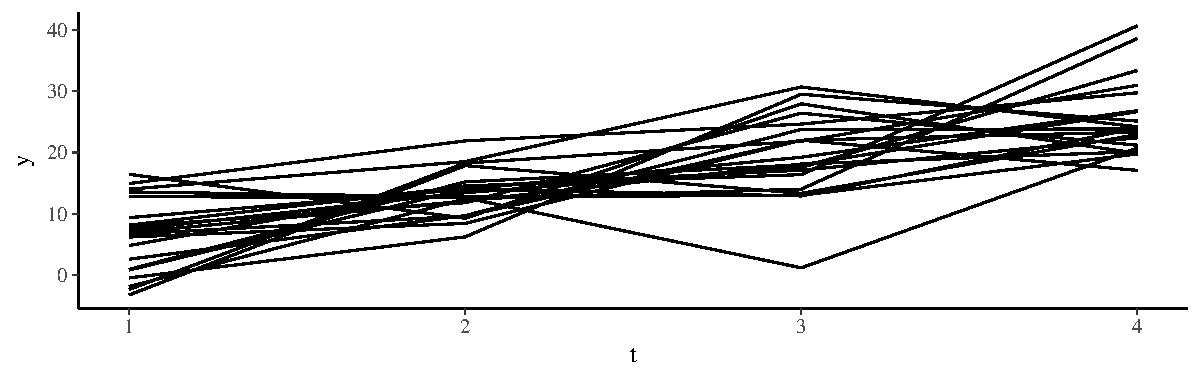
\includegraphics[width=\textwidth-3cm]{figure/ch04_figsimdata_repeated_unstruct-1} 

}


\begin{kframe}\begin{alltt}
\hlcom{# Bayesian framework}

\hlstd{Y} \hlkwb{<-} \hlkwd{matrix}\hlstd{(df[,}\hlstr{'y'}\hlstd{],} \hlnum{20}\hlstd{,} \hlnum{4}\hlstd{,} \hlkwc{byrow}\hlstd{=F)}
\hlstd{x1} \hlkwb{<-} \hlkwd{matrix}\hlstd{(df[,}\hlstr{'x1'}\hlstd{],} \hlnum{20}\hlstd{,} \hlnum{4}\hlstd{,} \hlkwc{byrow}\hlstd{=F)}
\hlstd{x2} \hlkwb{<-} \hlkwd{matrix}\hlstd{(df[,}\hlstr{'x2'}\hlstd{],} \hlnum{20}\hlstd{,} \hlnum{4}\hlstd{,} \hlkwc{byrow}\hlstd{=F)}
\hlstd{x3} \hlkwb{<-} \hlkwd{matrix}\hlstd{(df[,}\hlstr{'x3'}\hlstd{],} \hlnum{20}\hlstd{,} \hlnum{4}\hlstd{,} \hlkwc{byrow}\hlstd{=F)}
\hlstd{x4} \hlkwb{<-} \hlkwd{matrix}\hlstd{(df[,}\hlstr{'x4'}\hlstd{],} \hlnum{20}\hlstd{,} \hlnum{4}\hlstd{,} \hlkwc{byrow}\hlstd{=F)}

\hlstd{N} \hlkwb{=} \hlnum{20} \hlcom{#subjects}
\hlstd{M} \hlkwb{=} \hlnum{4} \hlcom{# repeated measures}
\end{alltt}
\end{kframe}
\end{knitrout}


\begin{knitrout}
\definecolor{shadecolor}{rgb}{0.98, 0.98, 0.98}\color{fgcolor}\begin{kframe}
\begin{alltt}
\hlcom{#--------------------------------------------}

\hlstd{modelString} \hlkwb{<-} \hlstr{"model\{

# Likelihood
for(i in 1:N)\{
Y[i,1:M] ~ dmnorm(mu[i,1:M],Omega[1:M,1:M])
for(j in 1:M)\{
mu[i,j] <- beta0 + beta1*x1[i,j]+ beta2*x2[i,j]+ beta3*x3[i,j] + beta4*x4[i,j]  
\}\}

# Priors

Omega[1:M, 1:M] ~dwish(zRmat[1:M,1:M] , zRscal)
Sigma[1:M, 1:M] <- inverse(Omega)

beta0      ~ dnorm(0,0.001)
beta1      ~ dnorm(0,0.001)
beta2      ~ dnorm(0,0.001)
beta3      ~ dnorm(0,0.001)
beta4      ~ dnorm(0,0.001)

\}"}


\hlkwd{writeLines}\hlstd{( modelString ,} \hlkwc{con}\hlstd{=}\hlstr{"Jags-MultivariateNormal-model.txt"} \hlstd{)}

\hlstd{model} \hlkwb{<-} \hlkwd{jags.model}\hlstd{(}\hlkwd{textConnection}\hlstd{(modelString),}
                                                                                \hlkwc{data} \hlstd{=} \hlkwd{list}\hlstd{(}\hlkwc{Y}\hlstd{=Y,}\hlkwc{N}\hlstd{=N,}\hlkwc{M}\hlstd{=M,}\hlkwc{x1} \hlstd{= x1,} \hlkwc{x2} \hlstd{= x2,} \hlkwc{x3} \hlstd{= x3,} \hlkwc{x4} \hlstd{= x4,}     \hlkwc{zRscal} \hlstd{=} \hlkwd{ncol}\hlstd{(Y) ,}  \hlcom{# for dwish prior}
                                                                                                                                \hlkwc{zRmat} \hlstd{=} \hlkwd{diag}\hlstd{(}\hlkwc{x}\hlstd{=}\hlnum{1}\hlstd{,}\hlkwc{nrow}\hlstd{=}\hlkwd{ncol}\hlstd{(Y)) ),}
                                                                                \hlkwc{n.chains}\hlstd{=}\hlnum{3}\hlstd{)}
\end{alltt}
\begin{verbatim}
## Compiling model graph
##    Resolving undeclared variables
##    Allocating nodes
## Graph information:
##    Observed stochastic nodes: 20
##    Unobserved stochastic nodes: 6
##    Total graph size: 789
## 
## Initializing model
\end{verbatim}
\begin{alltt}
\hlstd{samp} \hlkwb{<-} \hlkwd{coda.samples}\hlstd{(model,}
                                                                                 \hlkwc{variable.names}\hlstd{=}\hlkwd{c}\hlstd{(}\hlstr{"beta1"}\hlstd{,}\hlstr{'beta2'}\hlstd{,} \hlstr{'beta3'}\hlstd{,} \hlstr{'beta4'} \hlstd{,}\hlstr{"Sigma"}\hlstd{),}
                                                                                 \hlkwc{n.iter}\hlstd{=}\hlnum{20000}\hlstd{,} \hlkwc{progress.bar}\hlstd{=}\hlstr{"none"}\hlstd{)}

\hlkwd{summary}\hlstd{(samp)}
\end{alltt}
\begin{verbatim}
## 
## Iterations = 1:20000
## Thinning interval = 1 
## Number of chains = 3 
## Sample size per chain = 20000 
## 
## 1. Empirical mean and standard deviation for each variable,
##    plus standard error of the mean:
## 
##              Mean    SD Naive SE Time-series SE
## Sigma[1,1]  5.807 2.107 0.008602        0.00955
## Sigma[2,1]  3.863 1.777 0.007254        0.00800
## Sigma[3,1]  2.775 2.306 0.009416        0.00980
## Sigma[4,1]  4.562 3.058 0.012483        0.01426
## Sigma[1,2]  3.863 1.777 0.007254        0.00800
## Sigma[2,2]  5.077 2.307 0.009418        0.01104
## Sigma[3,2]  2.912 2.776 0.011332        0.01241
## Sigma[4,2]  5.027 3.853 0.015731        0.01662
## Sigma[1,3]  2.775 2.306 0.009416        0.00980
## Sigma[2,3]  2.912 2.776 0.011332        0.01241
## Sigma[3,3] 11.218 5.084 0.020756        0.02137
## Sigma[4,3] 12.660 6.143 0.025080        0.02548
## Sigma[1,4]  4.562 3.058 0.012483        0.01426
## Sigma[2,4]  5.027 3.853 0.015731        0.01662
## Sigma[3,4] 12.660 6.143 0.025080        0.02548
## Sigma[4,4] 18.737 8.630 0.035230        0.03585
## beta1       1.153 0.194 0.000790        0.00155
## beta2       0.812 0.175 0.000716        0.00125
## beta3       2.438 0.440 0.001797        0.01002
## beta4       1.792 0.476 0.001941        0.01114
## 
## 2. Quantiles for each variable:
## 
##              2.5%    25%   50%    75% 97.5%
## Sigma[1,1]  3.047  4.384  5.40  6.760 10.92
## Sigma[2,1]  1.553  2.720  3.56  4.655  7.95
## Sigma[3,1] -0.587  1.440  2.51  3.809  7.63
## Sigma[4,1]  0.185  2.709  4.16  5.948 11.19
## Sigma[1,2]  1.553  2.720  3.56  4.655  7.95
## Sigma[2,2]  2.583  3.786  4.71  5.937  9.62
## Sigma[3,2] -0.250  1.597  2.63  3.912  7.59
## Sigma[4,2]  1.009  3.202  4.59  6.329 11.53
## Sigma[1,3] -0.587  1.440  2.51  3.809  7.63
## Sigma[2,3] -0.250  1.597  2.63  3.912  7.59
## Sigma[3,3]  5.930  8.491 10.45 13.038 20.72
## Sigma[4,3]  6.232  9.390 11.74 14.852 24.20
## Sigma[1,4]  0.185  2.709  4.16  5.948 11.19
## Sigma[2,4]  1.009  3.202  4.59  6.329 11.53
## Sigma[3,4]  6.232  9.390 11.74 14.852 24.20
## Sigma[4,4]  9.950 14.214 17.47 21.746 34.73
## beta1       0.769  1.025  1.15  1.282  1.53
## beta2       0.469  0.696  0.81  0.926  1.16
## beta3       1.562  2.147  2.44  2.733  3.29
## beta4       0.876  1.472  1.79  2.107  2.73
\end{verbatim}
\begin{alltt}
\hlcom{#LMG calculations}

\hlstd{samp} \hlkwb{<-} \hlkwd{coda.samples}\hlstd{(model,}
                                                                                 \hlkwc{variable.names}\hlstd{=}\hlkwd{c}\hlstd{(}\hlstr{"beta1"}\hlstd{,}\hlstr{'beta2'}\hlstd{,} \hlstr{'beta3'}\hlstd{,} \hlstr{'beta4'} \hlstd{,}\hlstr{"Sigma[1,1]"}\hlstd{,}\hlstr{"Sigma[2,2]"}\hlstd{,}\hlstr{"Sigma[3,3]"}\hlstd{,}\hlstr{"Sigma[4,4]"}\hlstd{),}
                                                                                 \hlkwc{n.iter}\hlstd{=}\hlnum{20000}\hlstd{,} \hlkwc{thin}\hlstd{=}\hlnum{20}\hlstd{,} \hlkwc{progress.bar}\hlstd{=}\hlstr{"none"}\hlstd{)}

\hlstd{post.sample} \hlkwb{<-} \hlstd{samp[[}\hlnum{1}\hlstd{]][,}\hlkwd{c}\hlstd{(}\hlnum{5}\hlopt{:}\hlnum{8}\hlstd{,} \hlnum{1}\hlopt{:}\hlnum{4}\hlstd{)]}

\hlstd{df.rtwos} \hlkwb{<-} \hlkwd{rtwos.marg}\hlstd{(df[,}\hlnum{2}\hlopt{:}\hlnum{5}\hlstd{], post.sample,} \hlnum{4}\hlstd{)} \hlcom{# 4 repeated measures}

\hlstd{LMG.Vals}\hlkwb{<-}\hlkwd{matrix}\hlstd{(}\hlnum{0}\hlstd{,} \hlnum{4}\hlstd{,} \hlkwd{dim}\hlstd{(df.rtwos)[}\hlnum{2}\hlstd{])}

\hlkwa{for}\hlstd{(i} \hlkwa{in} \hlnum{1}\hlopt{:}\hlkwd{dim}\hlstd{(df.rtwos)[}\hlnum{2}\hlstd{])\{}

        \hlstd{gofn}\hlkwb{<-}\hlstd{df.rtwos[,i]}

        \hlstd{obj.Gelman}\hlkwb{<-}\hlkwd{partition}\hlstd{(gofn,} \hlkwc{pcan} \hlstd{=} \hlnum{4}\hlstd{,} \hlkwc{var.names} \hlstd{=} \hlkwd{names}\hlstd{(df[,}\hlnum{2}\hlopt{:}\hlnum{5}\hlstd{]))}

        \hlstd{LMG.Vals[,i]}\hlkwb{=}\hlstd{obj.Gelman}\hlopt{$}\hlstd{IJ[,}\hlnum{1}\hlstd{]}
\hlstd{\}}

\hlcom{# posterior LMG distribution of each variable}
\hlkwd{quantile}\hlstd{(LMG.Vals[}\hlnum{1}\hlstd{,],} \hlkwd{c}\hlstd{(}\hlnum{0.025}\hlstd{,} \hlnum{0.5}\hlstd{,} \hlnum{0.975}\hlstd{))}
\end{alltt}
\begin{verbatim}
##  2.5%   50% 97.5% 
## 0.100 0.128 0.150
\end{verbatim}
\begin{alltt}
\hlkwd{quantile}\hlstd{(LMG.Vals[}\hlnum{2}\hlstd{,],} \hlkwd{c}\hlstd{(}\hlnum{0.025}\hlstd{,} \hlnum{0.5}\hlstd{,} \hlnum{0.975}\hlstd{))}
\end{alltt}
\begin{verbatim}
##   2.5%    50%  97.5% 
## 0.0987 0.1267 0.1462
\end{verbatim}
\begin{alltt}
\hlkwd{quantile}\hlstd{(LMG.Vals[}\hlnum{3}\hlstd{,],} \hlkwd{c}\hlstd{(}\hlnum{0.025}\hlstd{,} \hlnum{0.5}\hlstd{,} \hlnum{0.975}\hlstd{))}
\end{alltt}
\begin{verbatim}
##  2.5%   50% 97.5% 
## 0.166 0.213 0.245
\end{verbatim}
\begin{alltt}
\hlkwd{quantile}\hlstd{(LMG.Vals[}\hlnum{4}\hlstd{,],} \hlkwd{c}\hlstd{(}\hlnum{0.025}\hlstd{,} \hlnum{0.5}\hlstd{,} \hlnum{0.975}\hlstd{))}
\end{alltt}
\begin{verbatim}
##  2.5%   50% 97.5% 
## 0.167 0.213 0.240
\end{verbatim}
\end{kframe}
\end{knitrout}









% LaTeX file for Chapter 05






\chapter{Other variable importance metrics in the Bayesian framework}

Different variable importance metrics exist. The conditional variance formula allowed us to calculate the $\Rtwo$ of the submodels from the posterior sample of the full model. The focus of this master thesis was on the LMG formula. For each posterior sample the LMG formula can be applied for the submodels of each posterior sample. A lot of the variable importance metrics are based on the $\Rtwo$ of the full model compared to the submodels. Instead of the LMG formula we could as well have used another variable importance metric after we have calculated the $\Rtwo$ of all the submodels. Commonality and dominance analysis seem to be interesting extensions of the LMG framework. Both provide besides the LMG information some other information about the variance decomposition of the predictors. The relaimpo package provides some more bootstrap options like pariwise differences that could also be easily transfered to the Bayesian framework. 


 
\section{Conclusion}

The Bayesian framworks provides us with a nice option to include the uncertainty about parameters. Posterior distributions of the parameters allow us to calculate a distribution of $\Rtwo$ values for each model. Using  the conditional variance formula allowd us to calculate the $\Rtwo$ of all the submodels from the posterior parameter distributions of the full model. Instead of fitting $2^
{p-1}$ models, only the full model needs to be fitted. Doing it this way has some nice properties. The interdependence of the submodels to each other is respected. The $\Rtwo$ of the submodels does not decrease when adding predictors. The non-negativity of the shares is therefore respected in the LMG formula. This property of using the conditional variance formula is also interesting when the LMG formula is applied to random intercept models fitted by maximum likelihood. 

A disadventage about calculating the $\Rtwo$ of all the submodels with the conditional variance formula  seems to be the restriction to the linear model. Although this may be a topic of further research.

Assuming non-stochastic or stochastic predictors can have a big impact on the the uncertainty of the explained variance and the LMG values. Although the posterior regression parameter distribtuions is the same in both cases (under some assumptions described in chapter ...) the explainened variance of a model is directly dependent on the covarinace matrix. Inference about the covariance of the predictors $\X$ is therefore an important part when stochastic predictors are assumed. However, this does in general not seem to be an easy problem. Non-parametric bootstrap provides a practical solution. 


 


. 


% LaTeX file for appendix






\chapter{Appendix}

\cleardoublepage
\phantomsection
\addtocontents{toc}{\protect \vspace*{10mm}}
\addcontentsline{toc}{chapter}{\bfseries Bibliography}


\bibliographystyle{mywiley} 
\bibliography{biblio}

\cleardoublepage

\end{document}



%%% Local Variables:
%%% ispell-local-dictionary: "en_US"
%%% End:
